\subsection{Reference satellites}

\subsubsection{NPP-375D}

\begin{frame}
  NPP-375D
\end{frame}

\begin{frame}
  \frametitle{Time series trend (with smoothing)}
  \begin{figure}
    \centering
    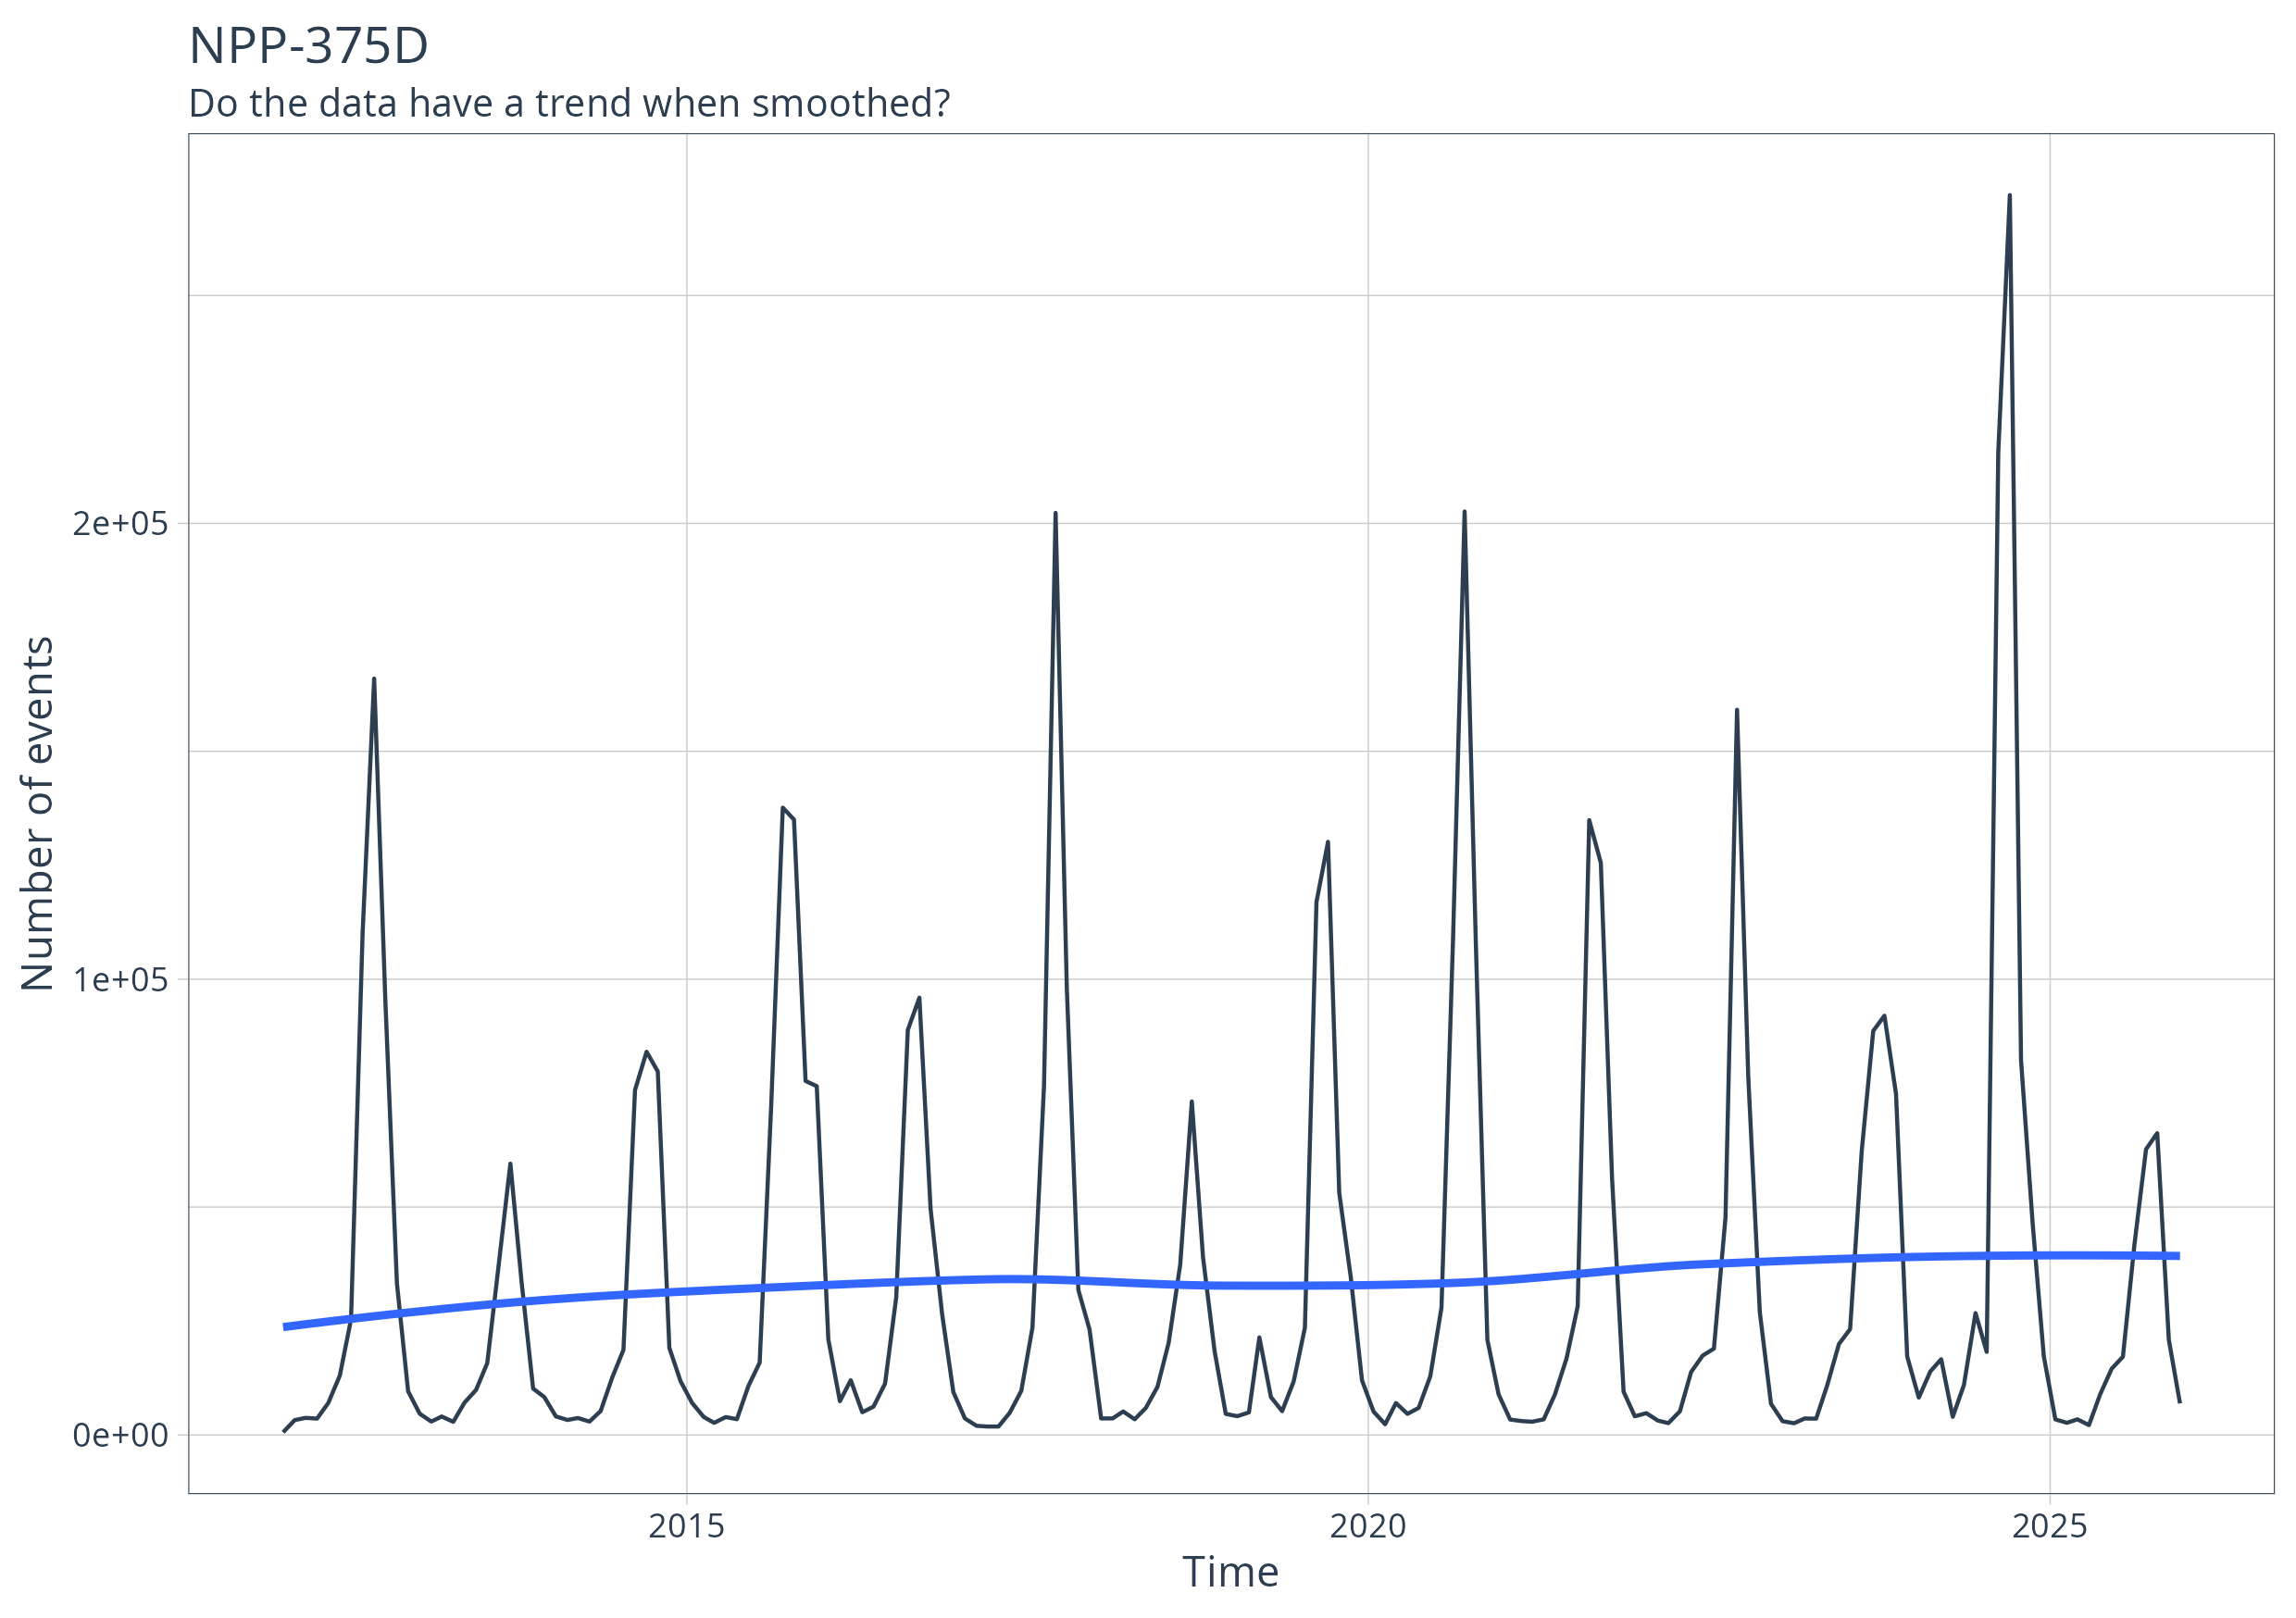
\includegraphics[scale=0.35]{figures/plot_trend_smoothing_NPP-375D.png}
    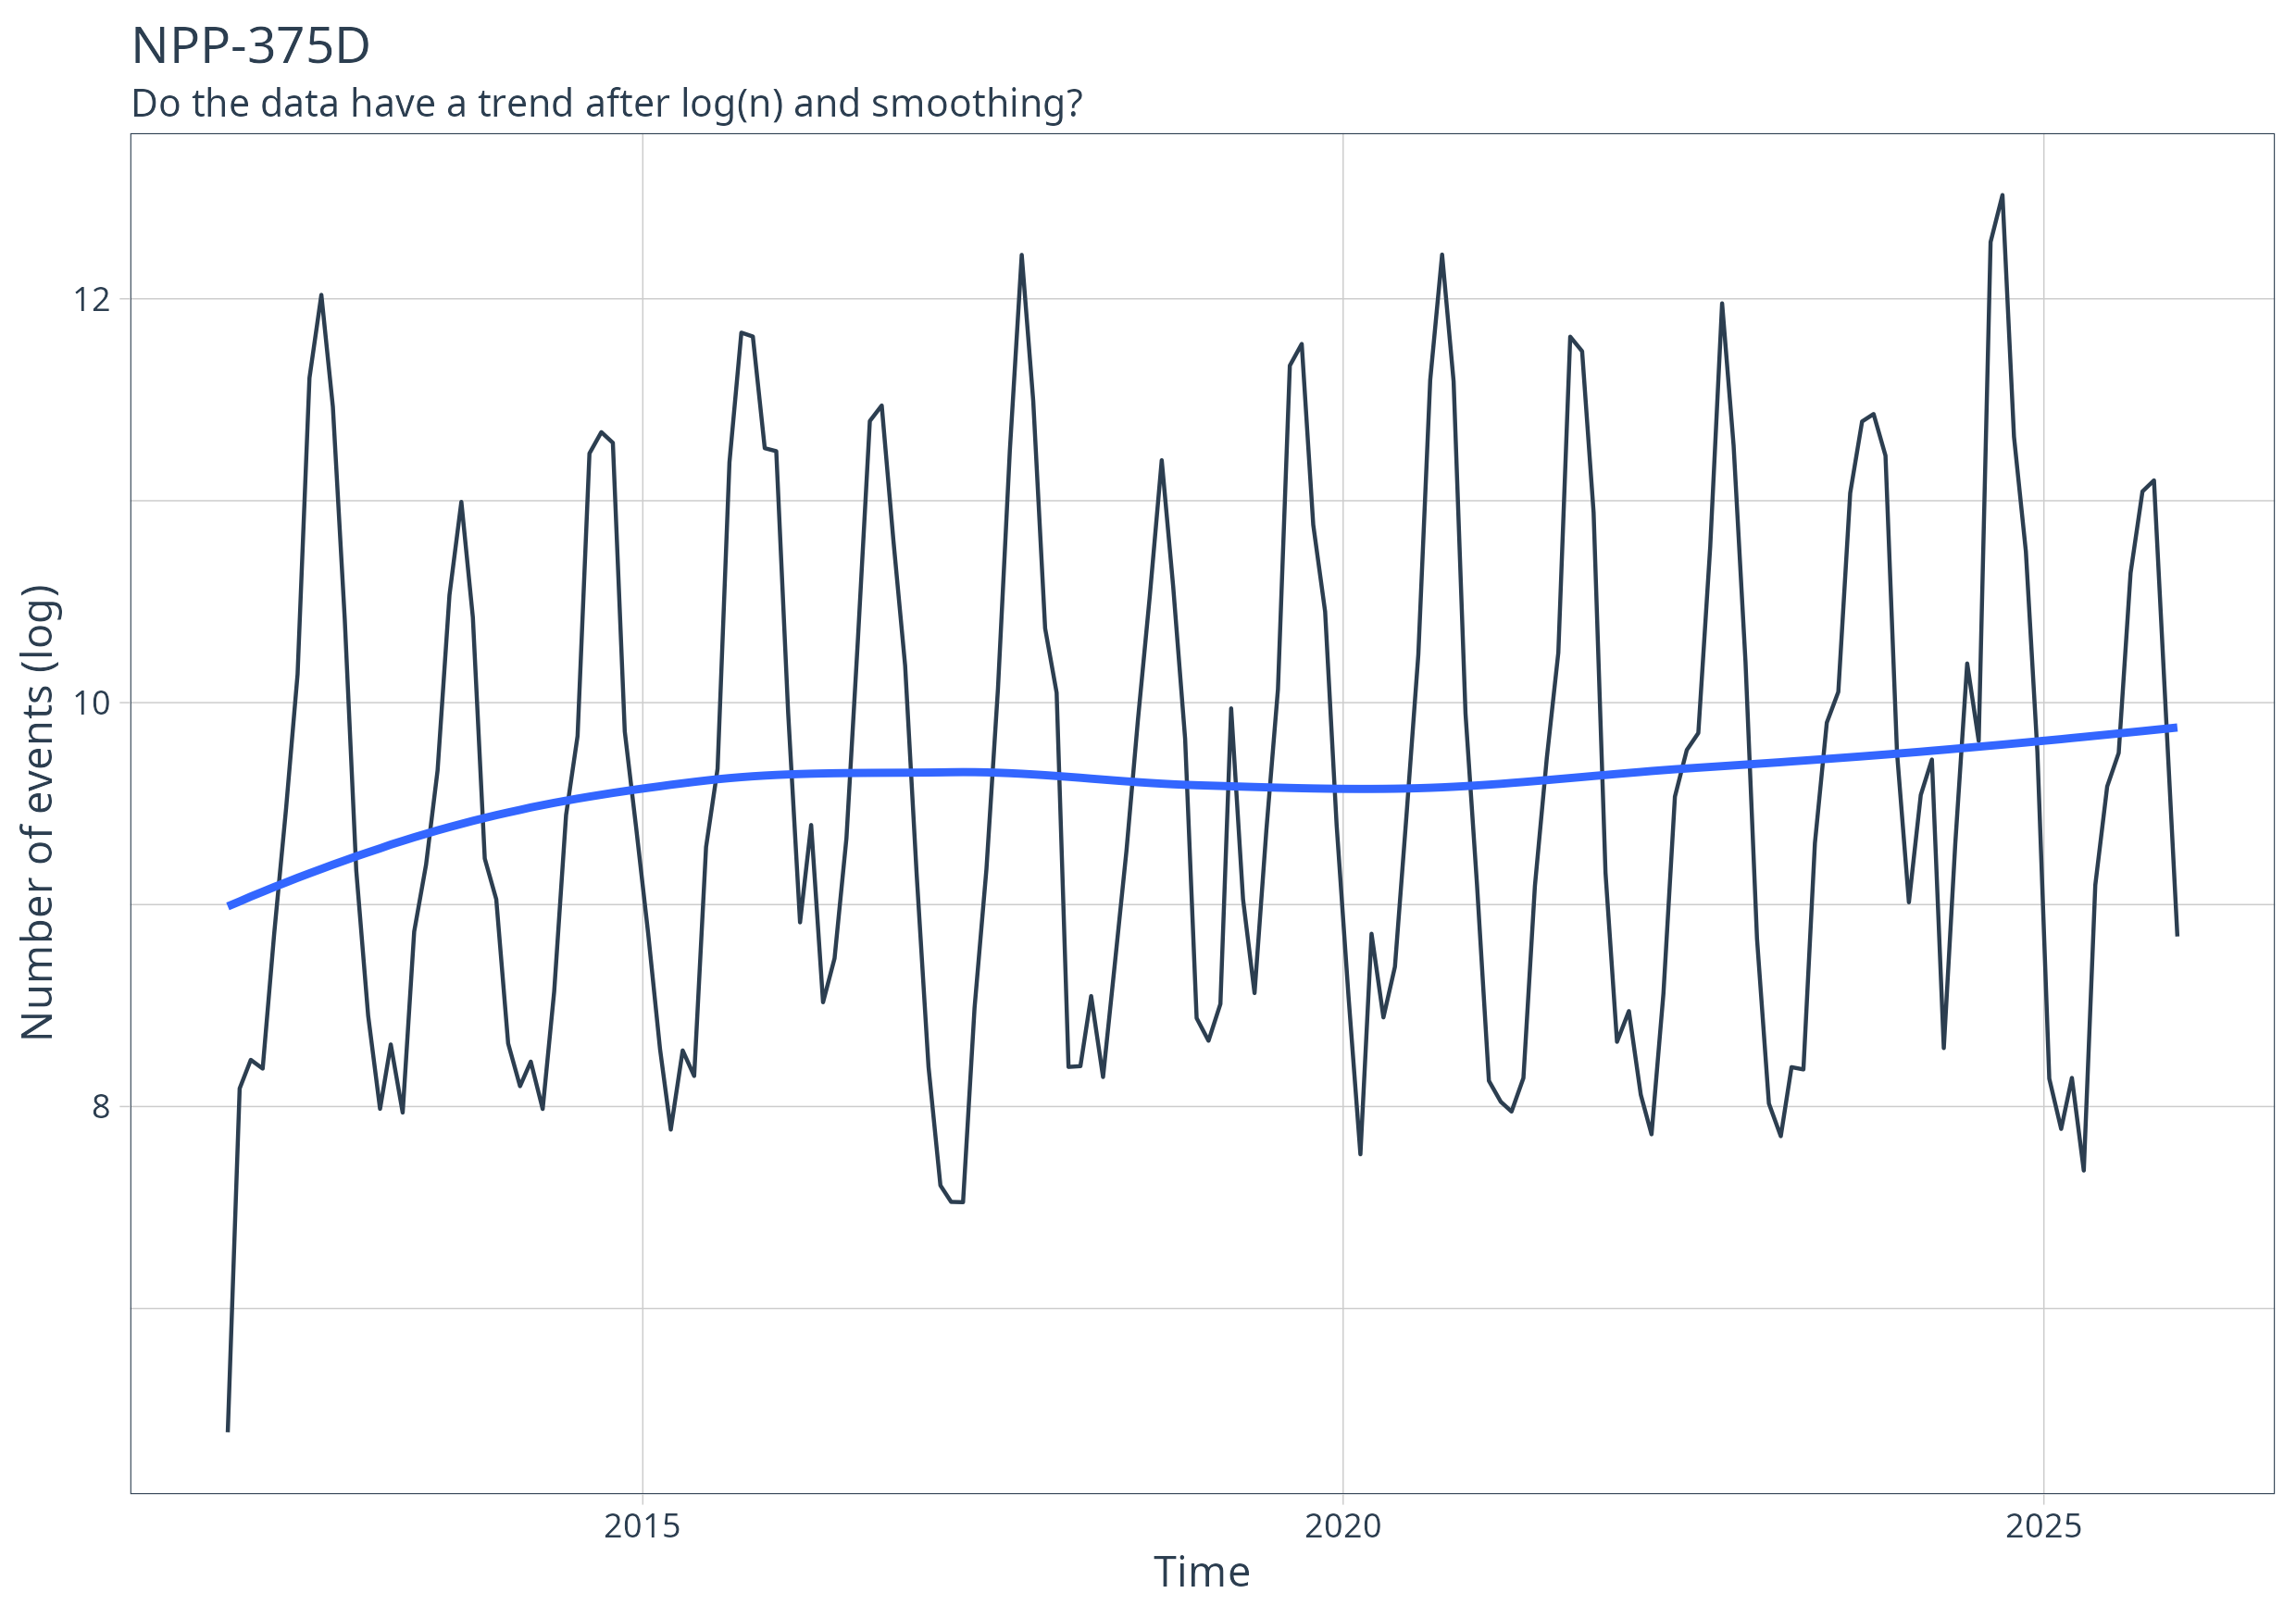
\includegraphics[scale=0.35]{figures/plot_trend_smoothing_log_NPP-375D.png}
    \caption{Do the data have a trend when smoothed? (data and data log to the
    left).}
  \end{figure}
\end{frame}

\begin{frame}
  \frametitle{Time series autocorrelation}
  \begin{figure}
    \centering
    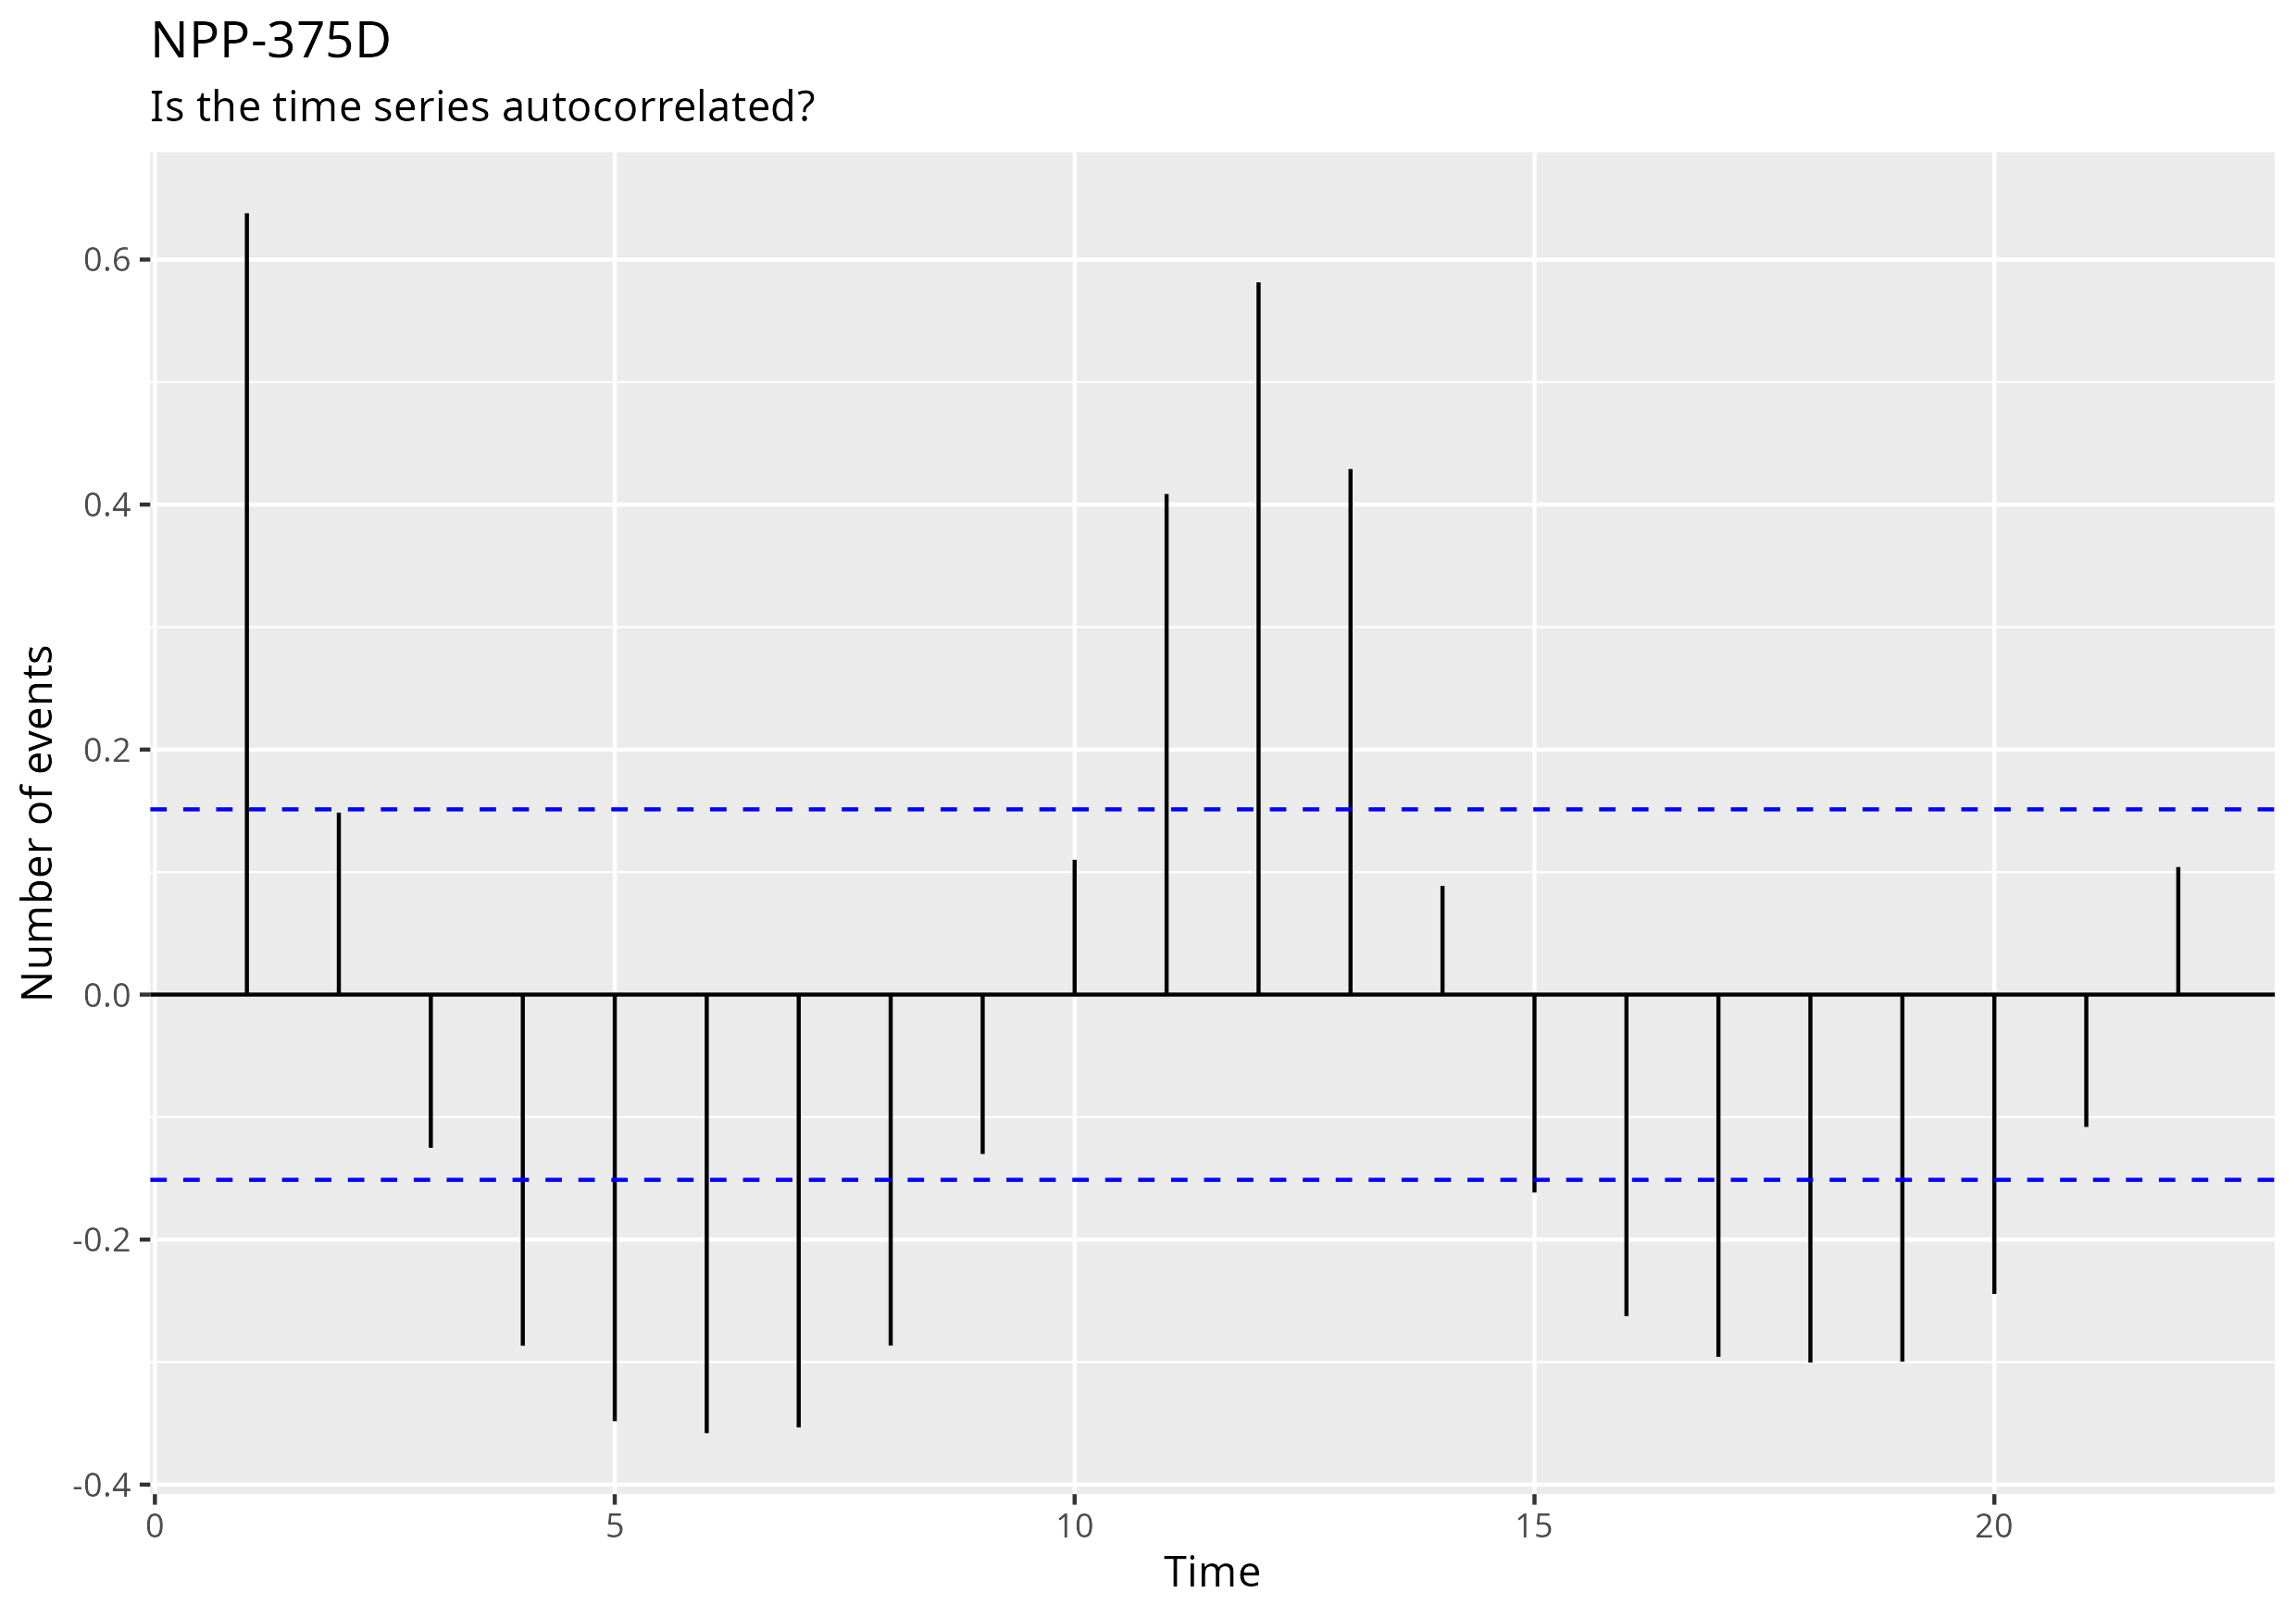
\includegraphics[scale=0.45]{figures/plot_autocorrelation_NPP-375D.png}
    \caption{Is the time series autocorrelated?}
  \end{figure}
\end{frame}

\begin{frame}
  \frametitle{Time series trend}
  \begin{figure}
    \centering
    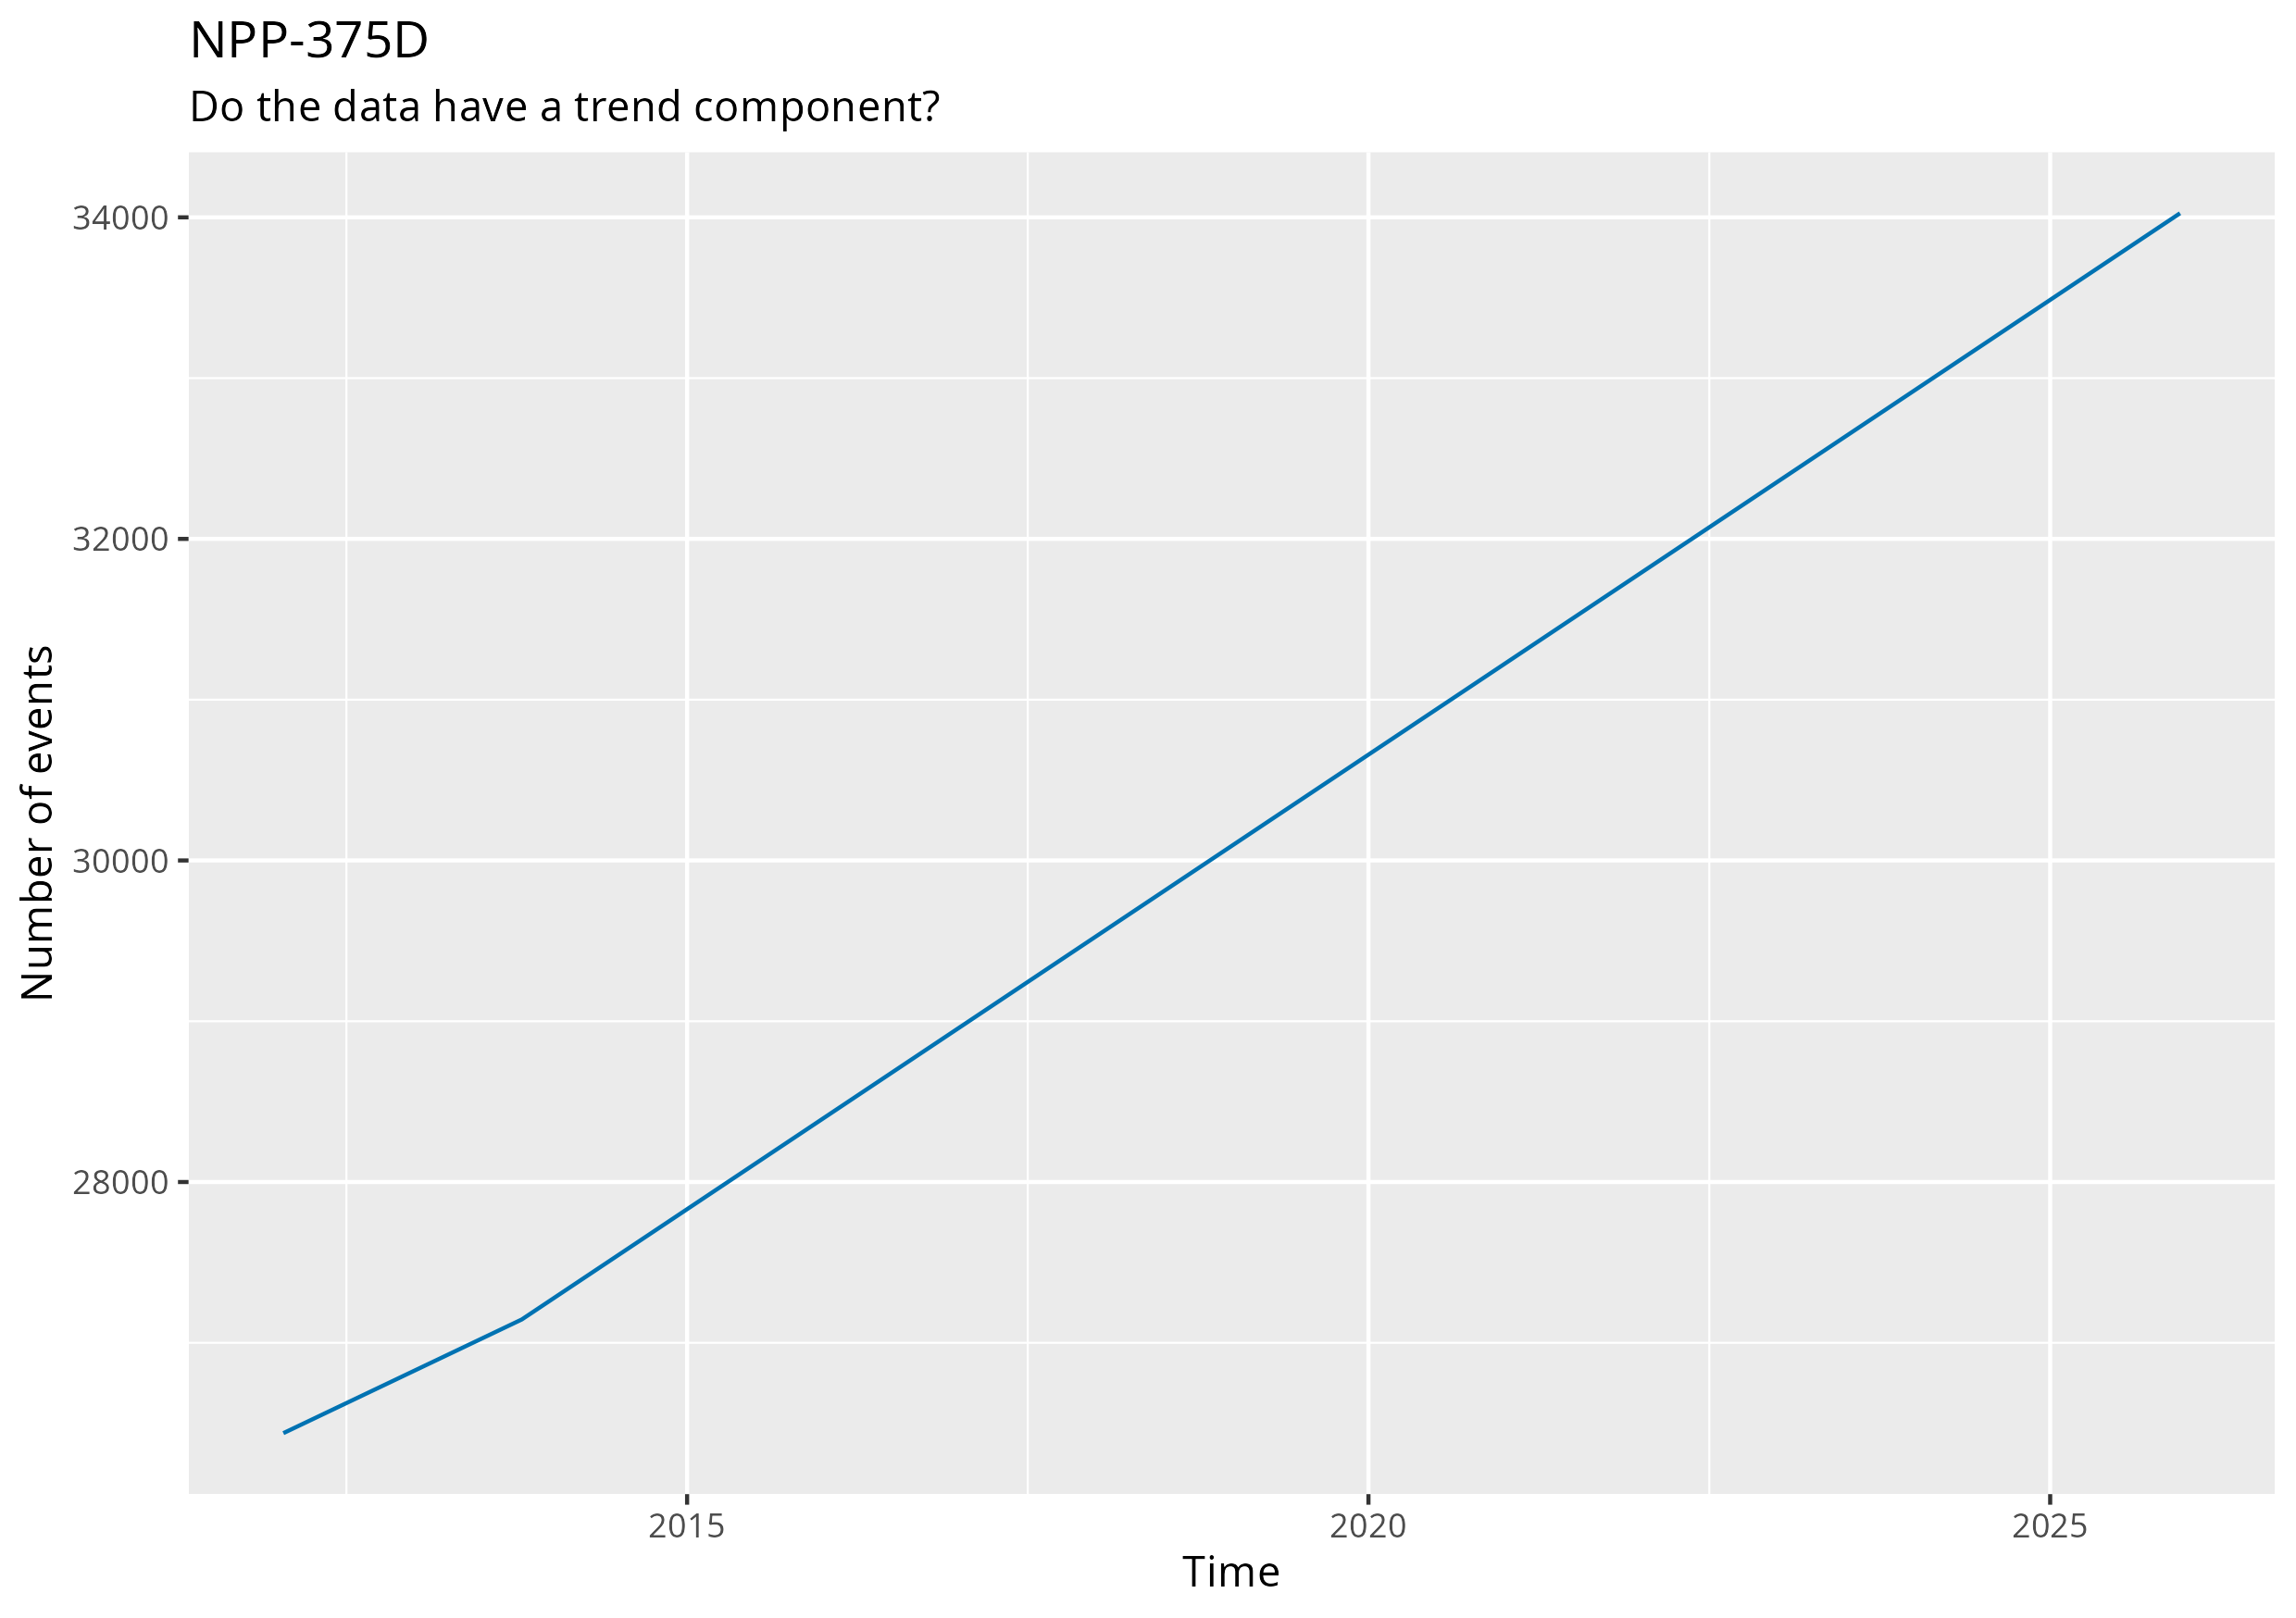
\includegraphics[scale=0.5]{figures/plot_component_trend_NPP-375D.png}
    \caption{Do the data have a trend component?}
  \end{figure}
\end{frame}

\begin{frame}
  \frametitle{Time series seasonality}
  \begin{figure}
    \centering
    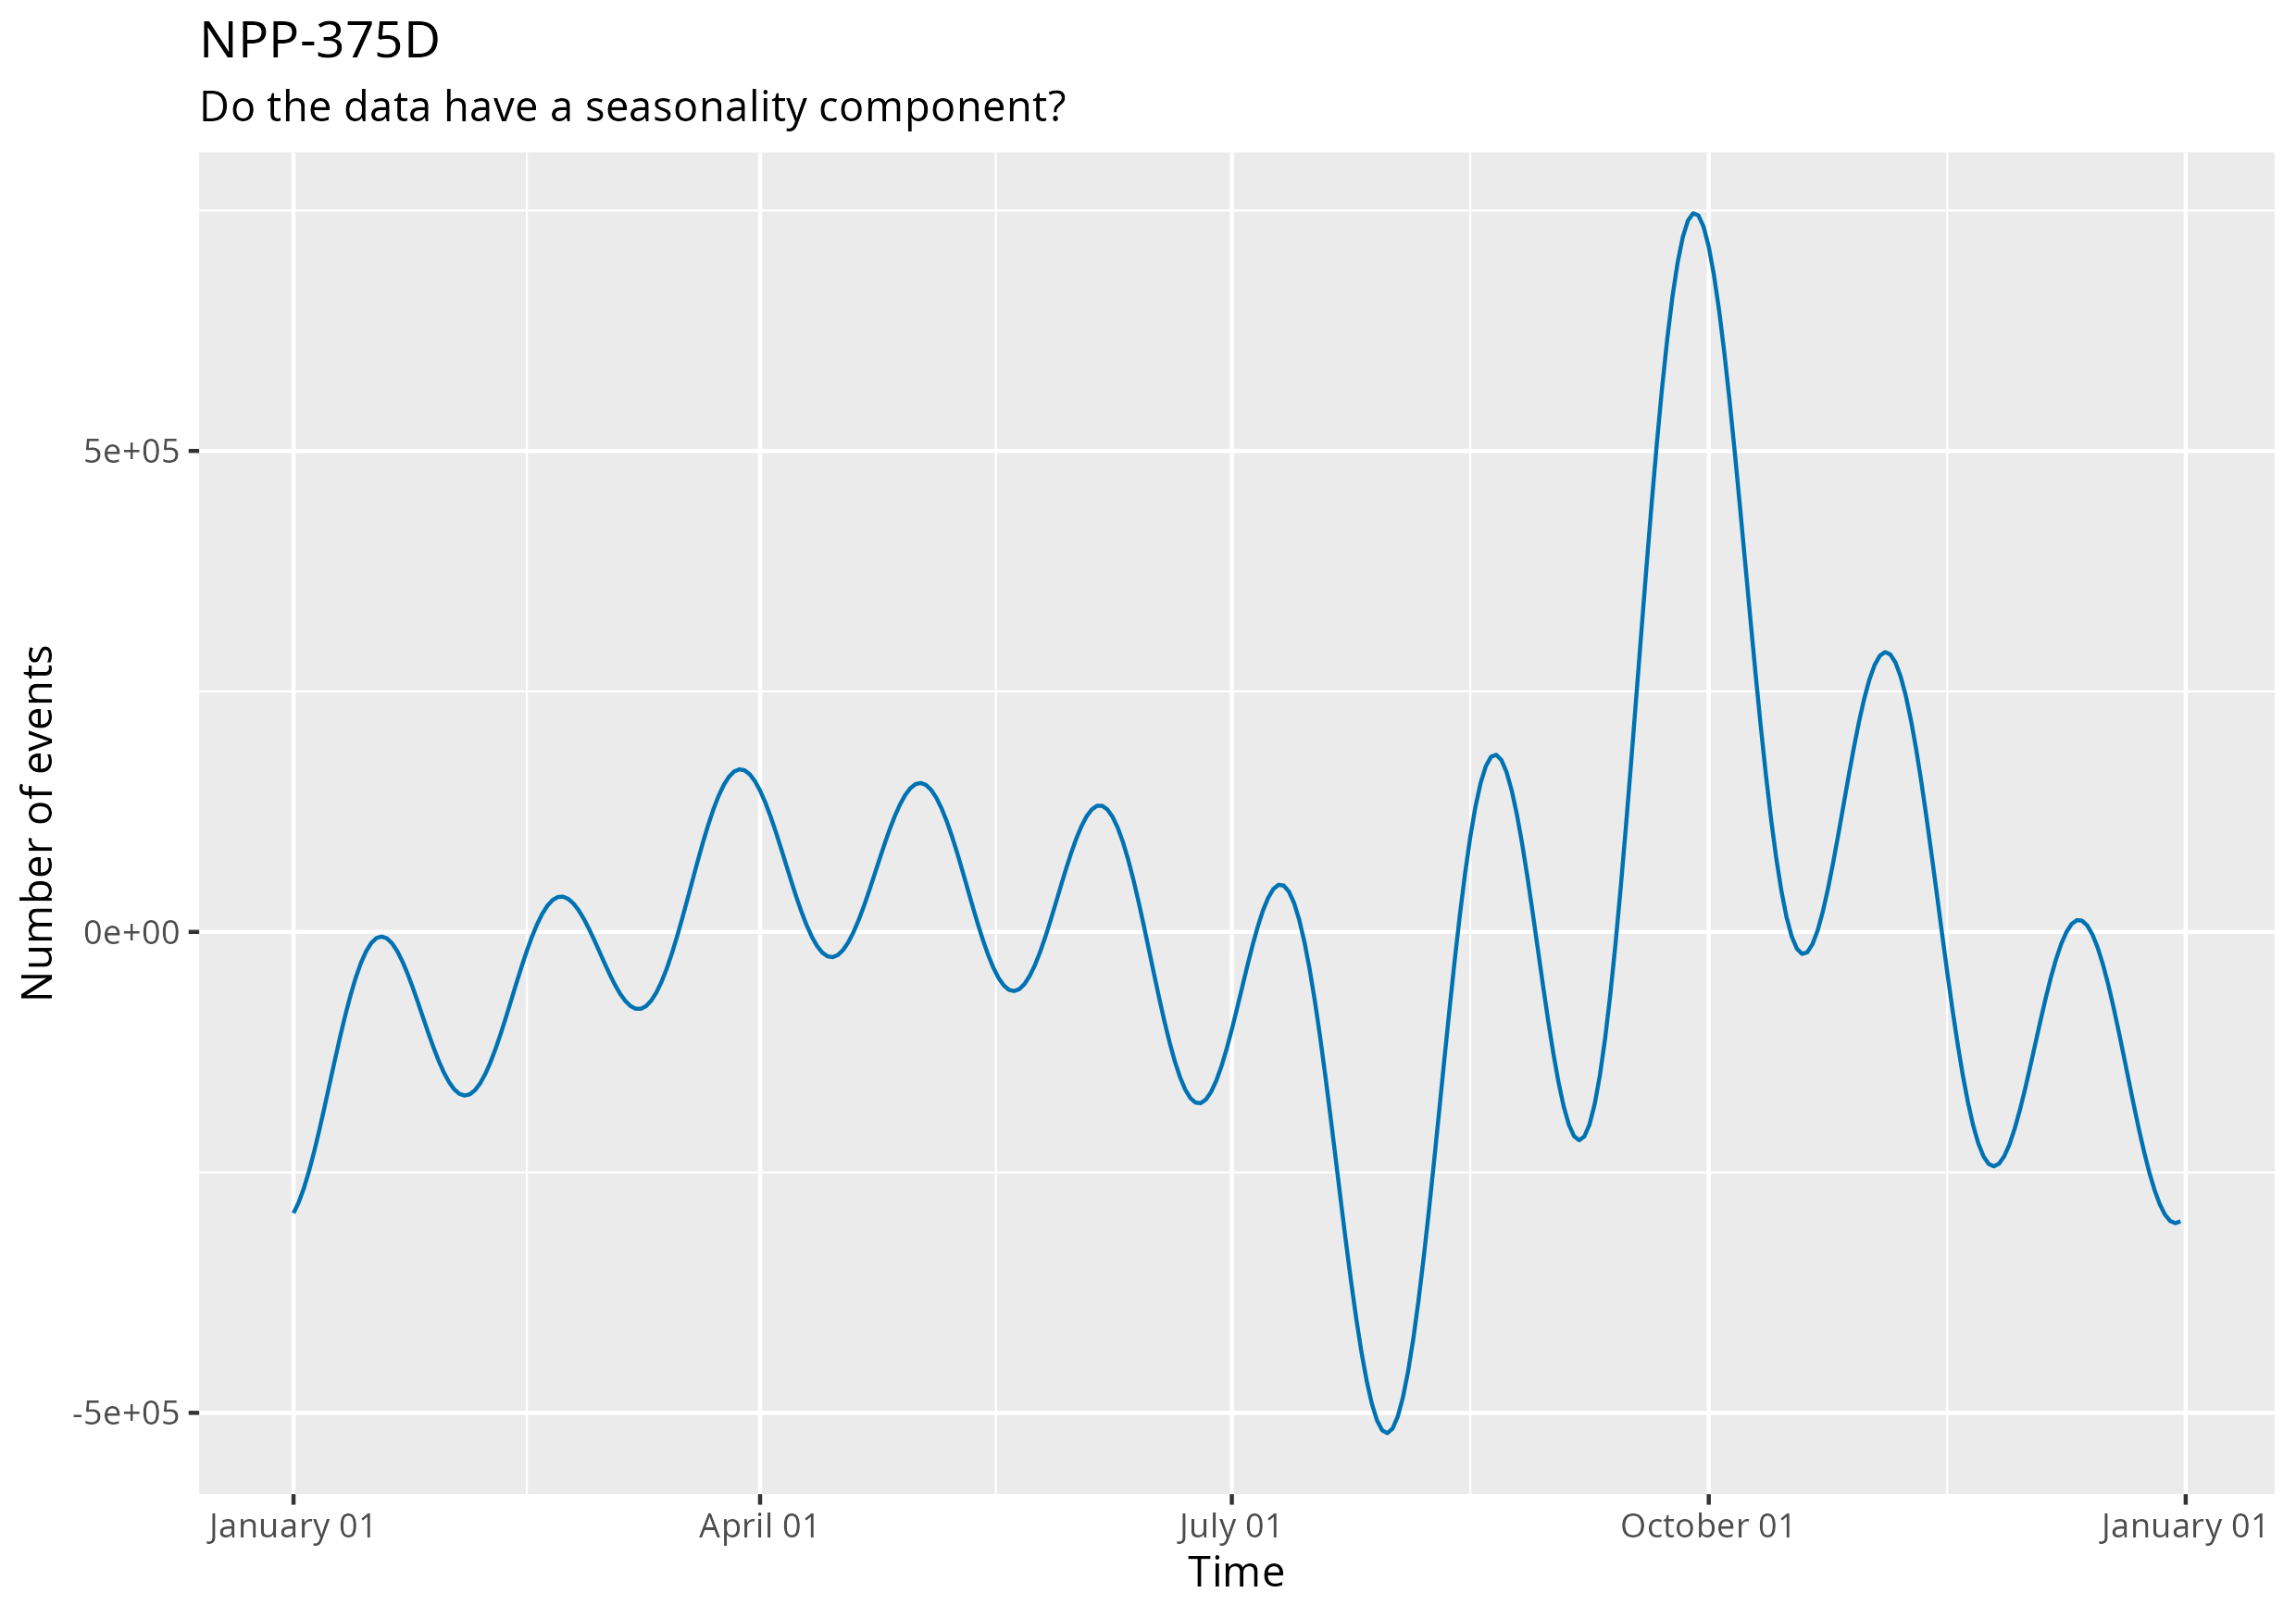
\includegraphics[scale=0.45]{figures/plot_component_seasonality_NPP-375D.png}
    \caption{Do the data have a seasonality component?}
  \end{figure}
\end{frame}

\begin{frame}
  \frametitle{Time series versus forecast}
  \begin{figure}
    \centering
    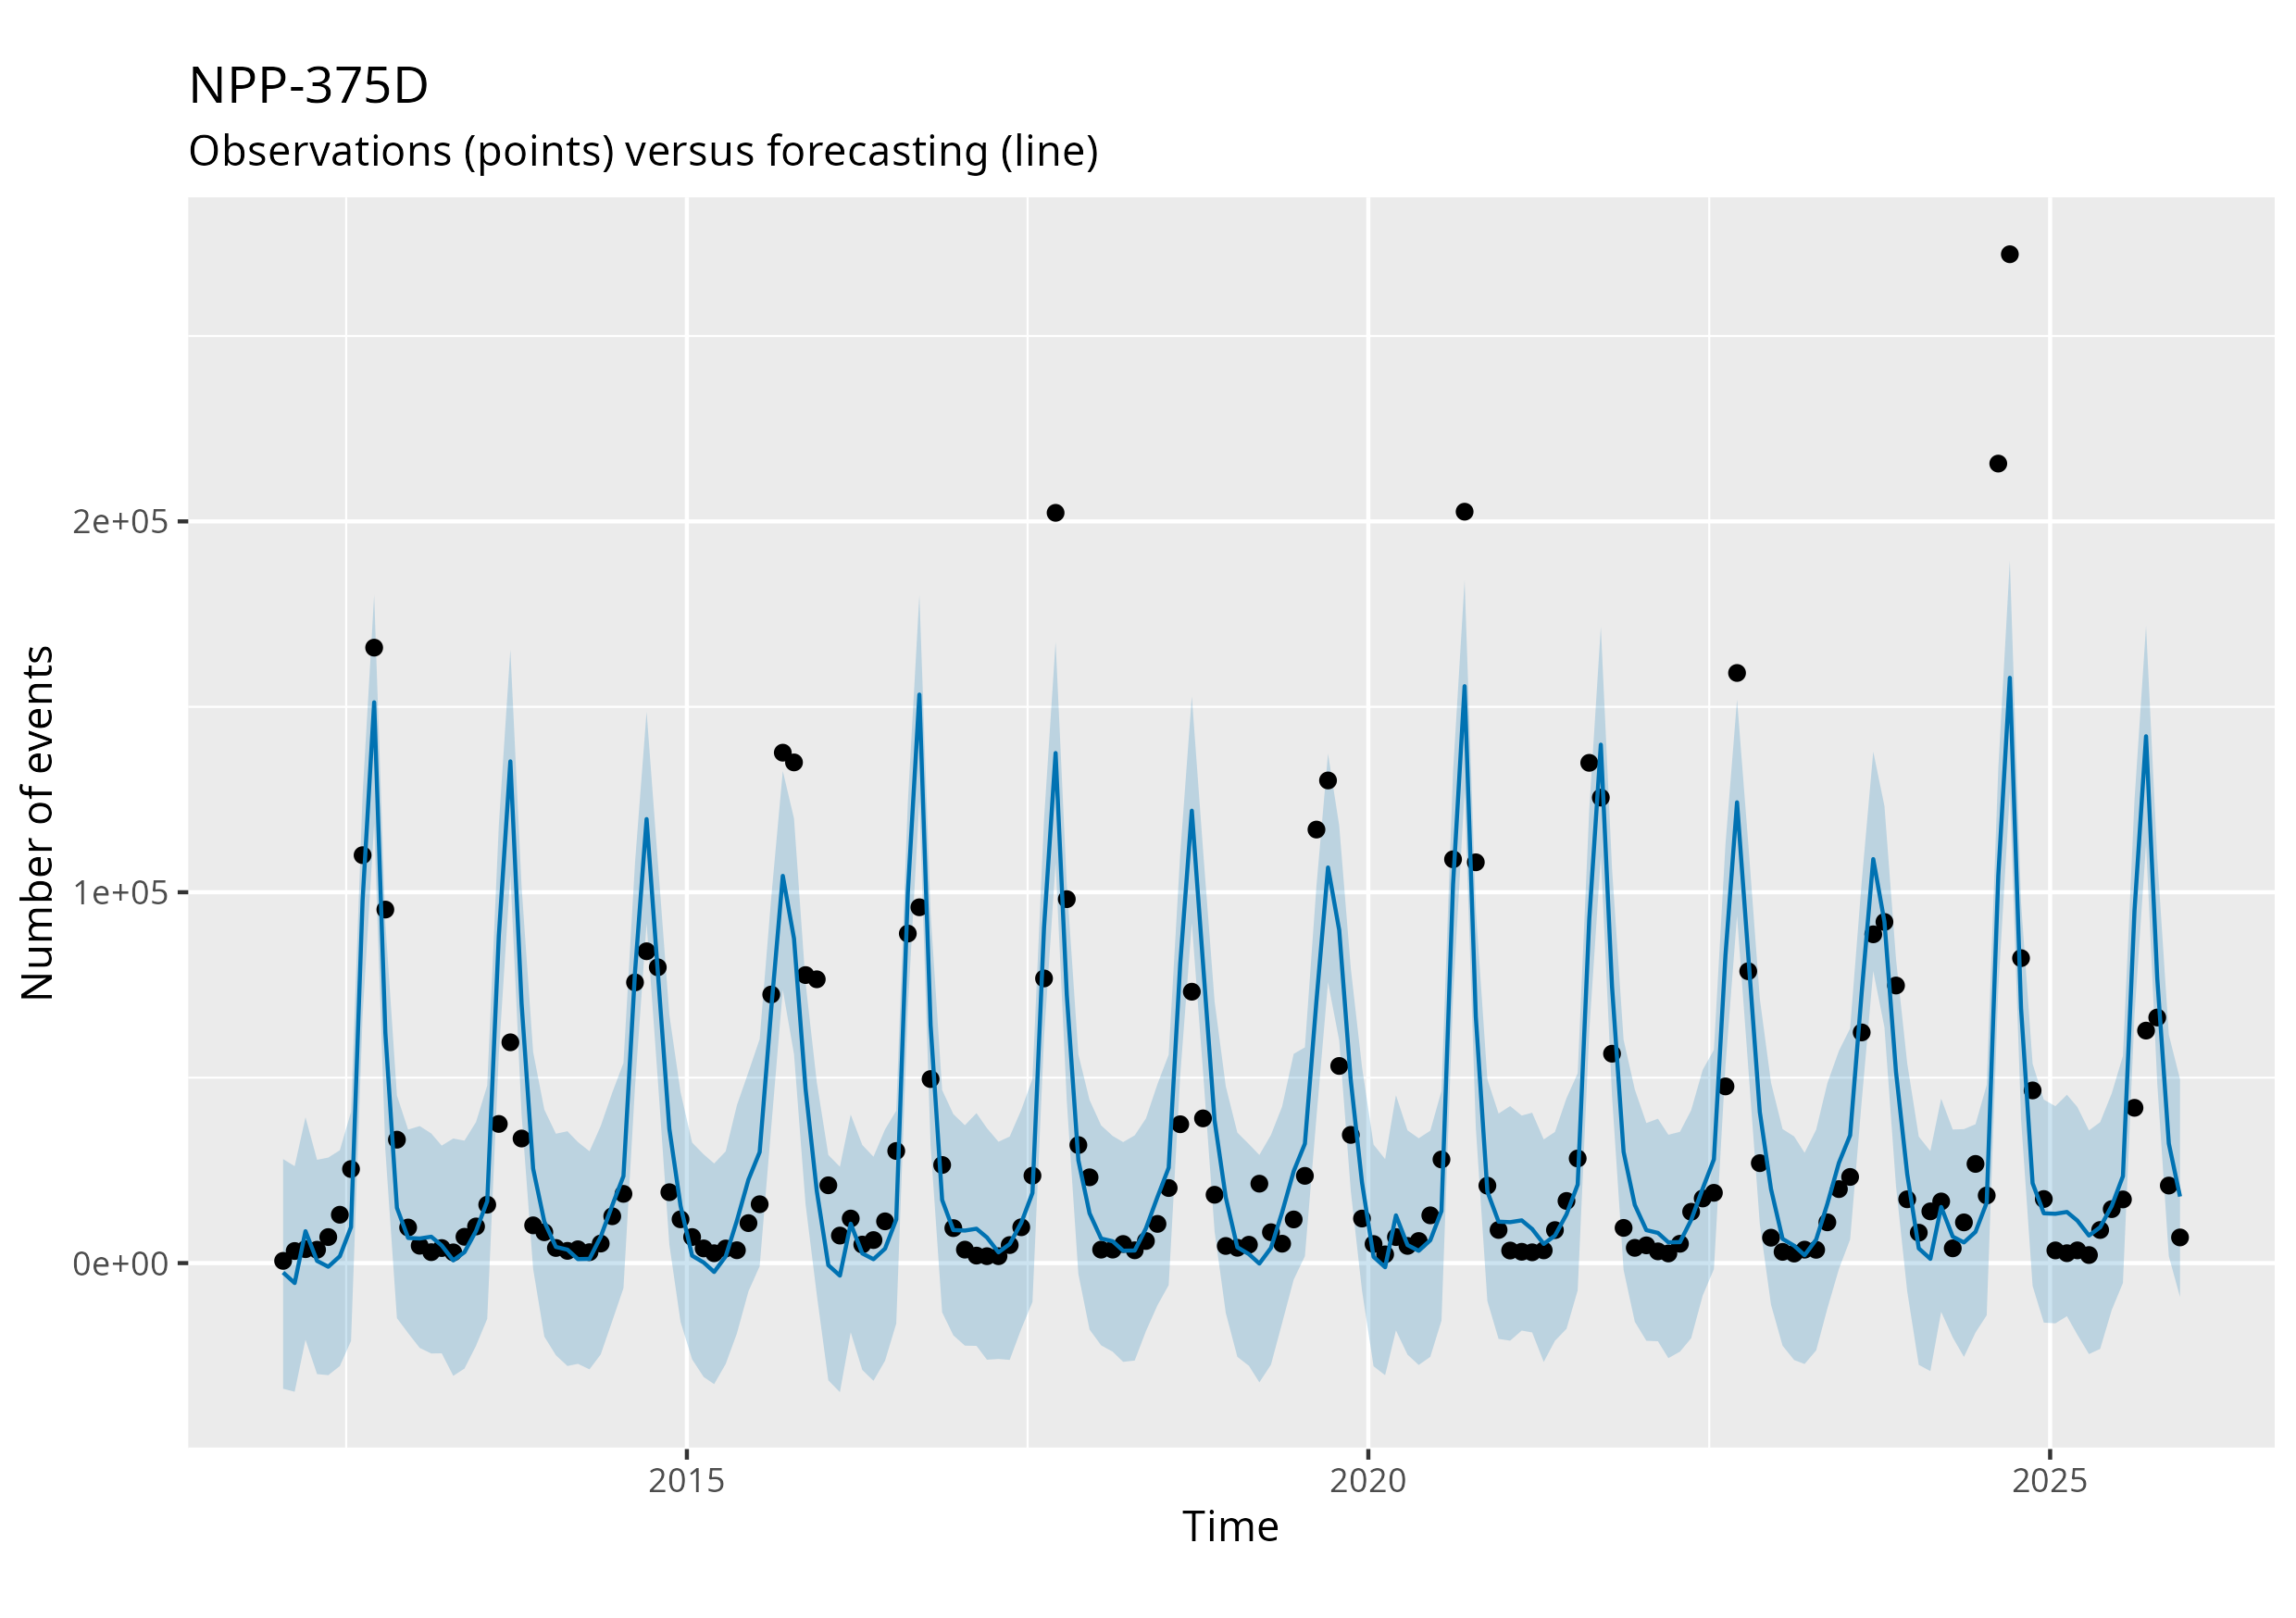
\includegraphics[scale=0.45]{figures/plot_model_forecast_NPP-375D.png}
    \caption{Observations (black dots) and model (blue line) with a 95\%
    confidence interval (gray shadow).}
  \end{figure}
\end{frame}

\begin{frame}
  \frametitle{Time series versus forecast}
  \begin{figure}
    \centering
    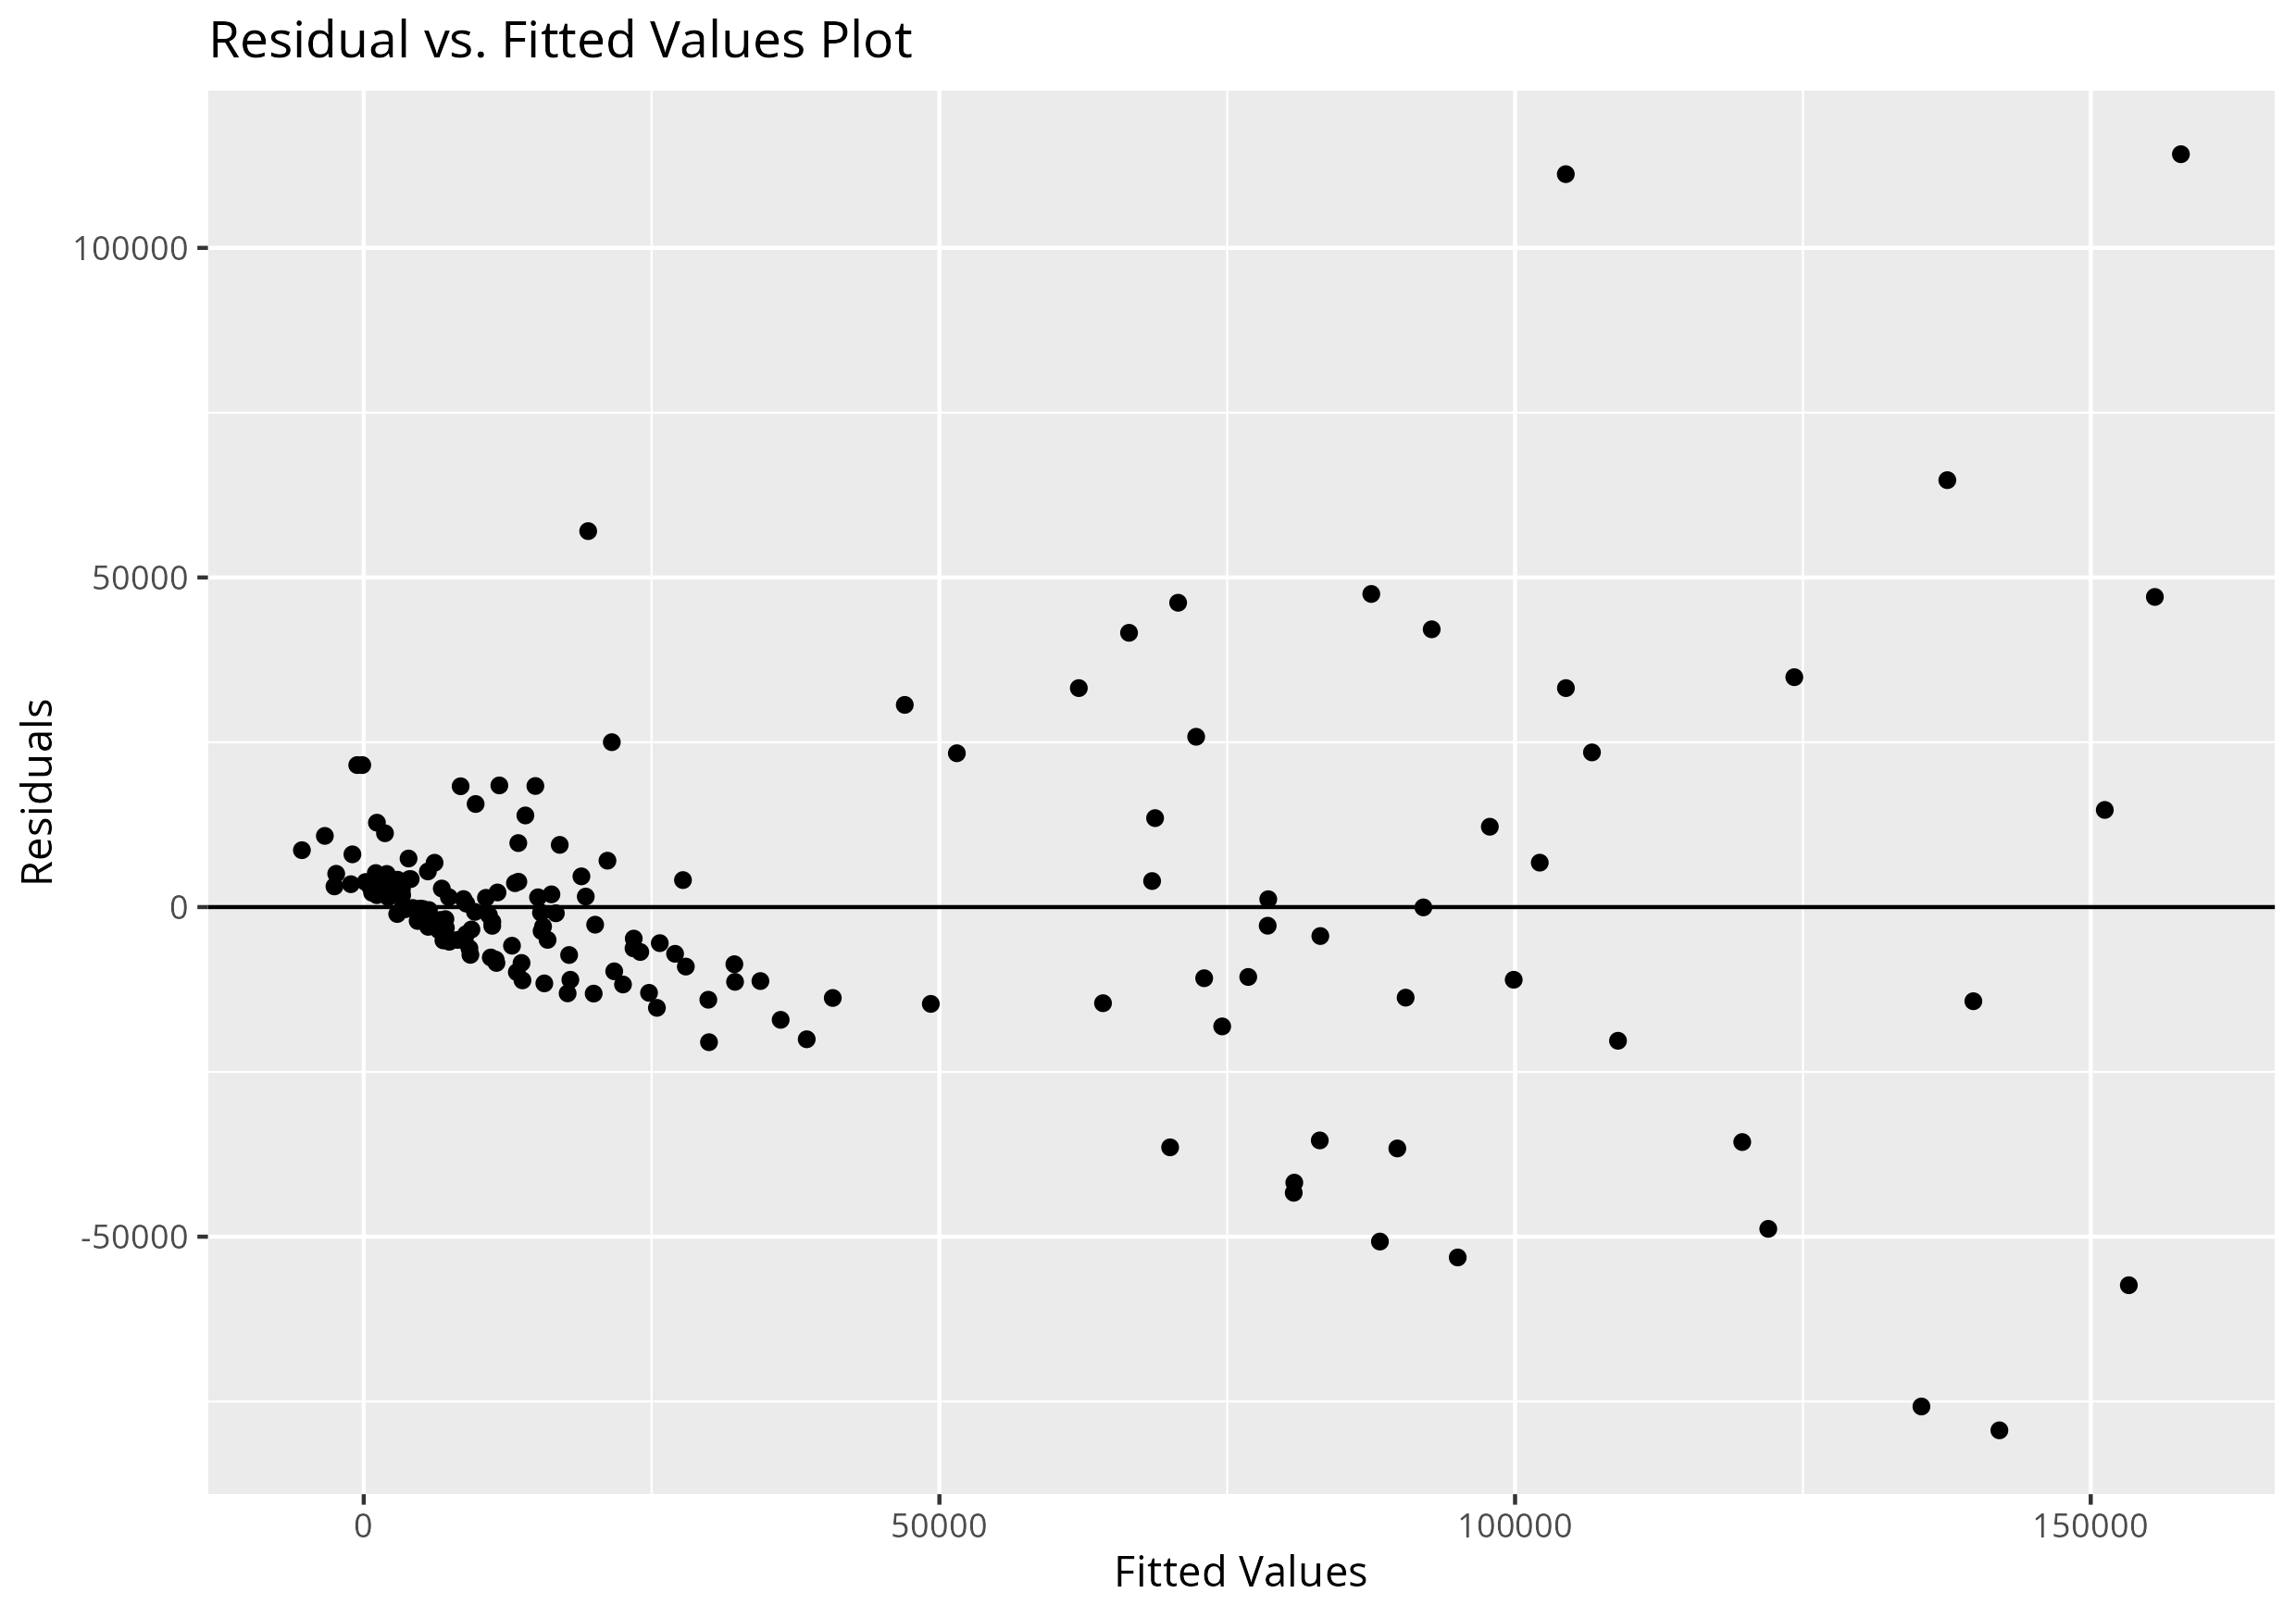
\includegraphics[scale=0.45]{figures/plot_residuals_NPP-375D.png}
    \caption{Large observations of fire foci have larger residuals.}
  \end{figure}
\end{frame}

\begin{frame}
  \frametitle{Time series versus forecast}
  \begin{figure}
    \centering
    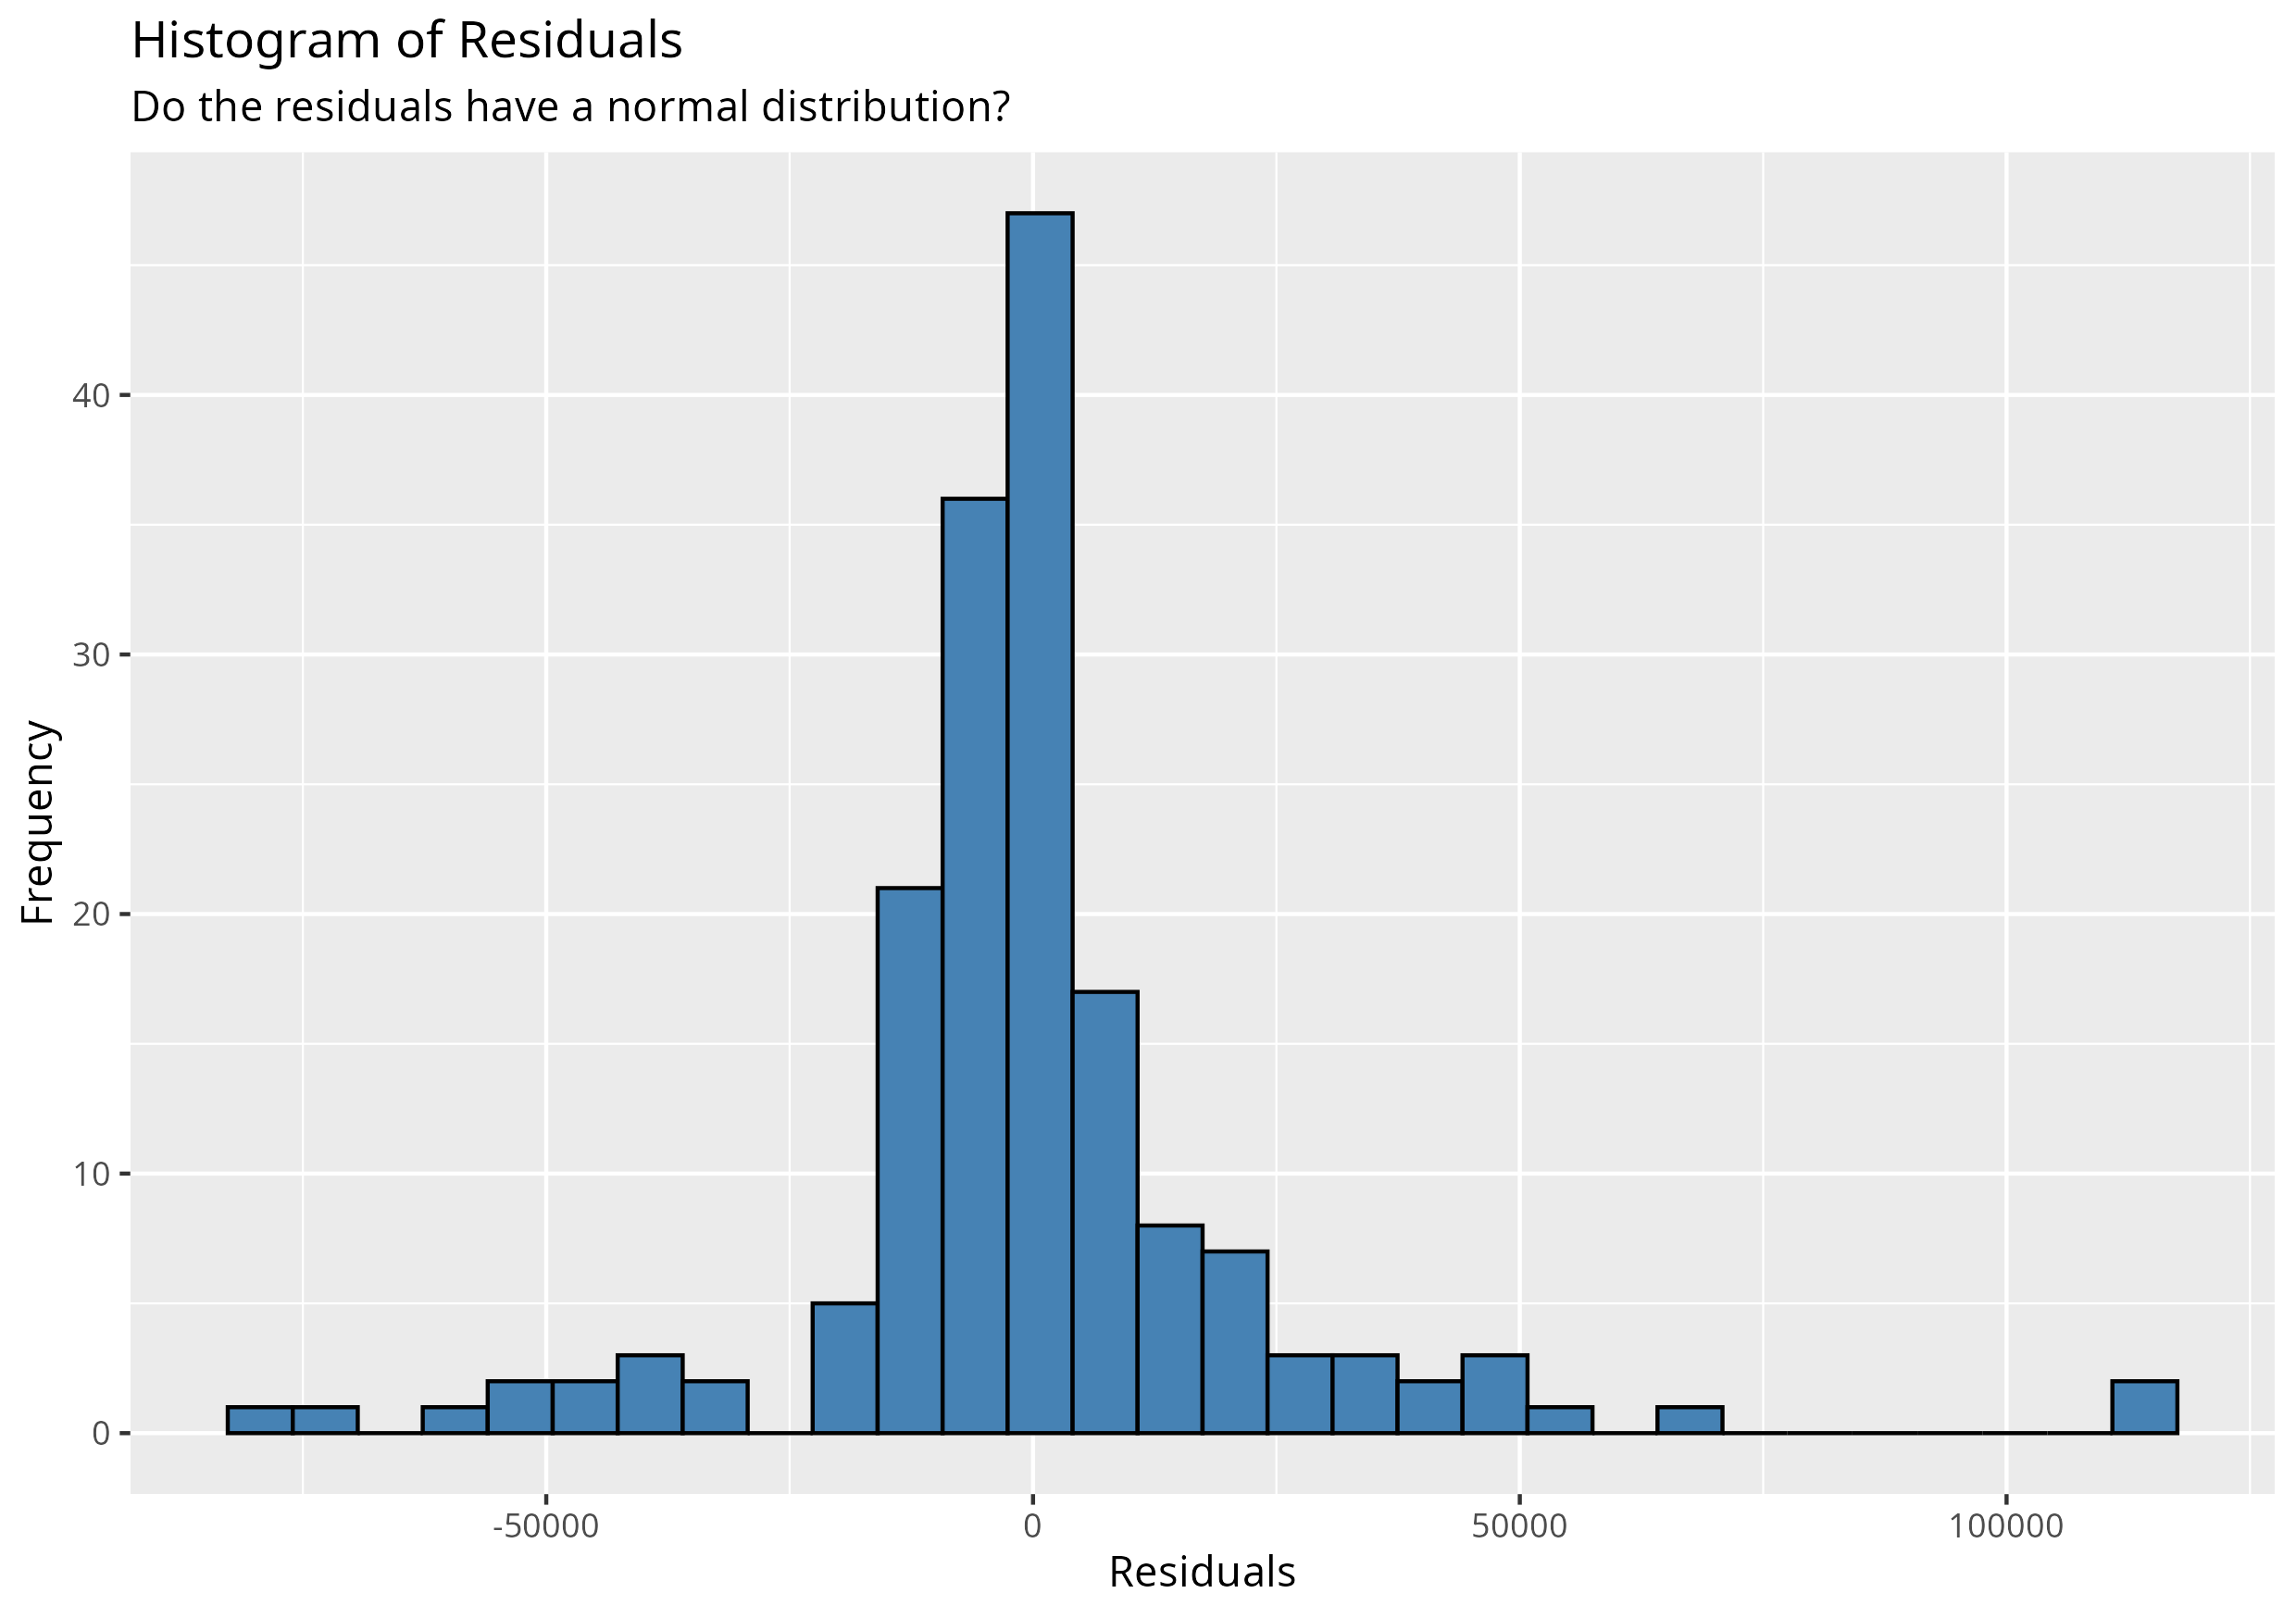
\includegraphics[scale=0.45]{figures/plot_residuals_hist_NPP-375D.png}
    \caption{Do the residuals have a normal distribution?}
  \end{figure}
\end{frame}

\subsubsection{NPP-375-PM}

\begin{frame}
  NPP-375-PM
\end{frame}

\begin{frame}
  \frametitle{Time series trend (with smoothing)}
  \begin{figure}
    \centering
    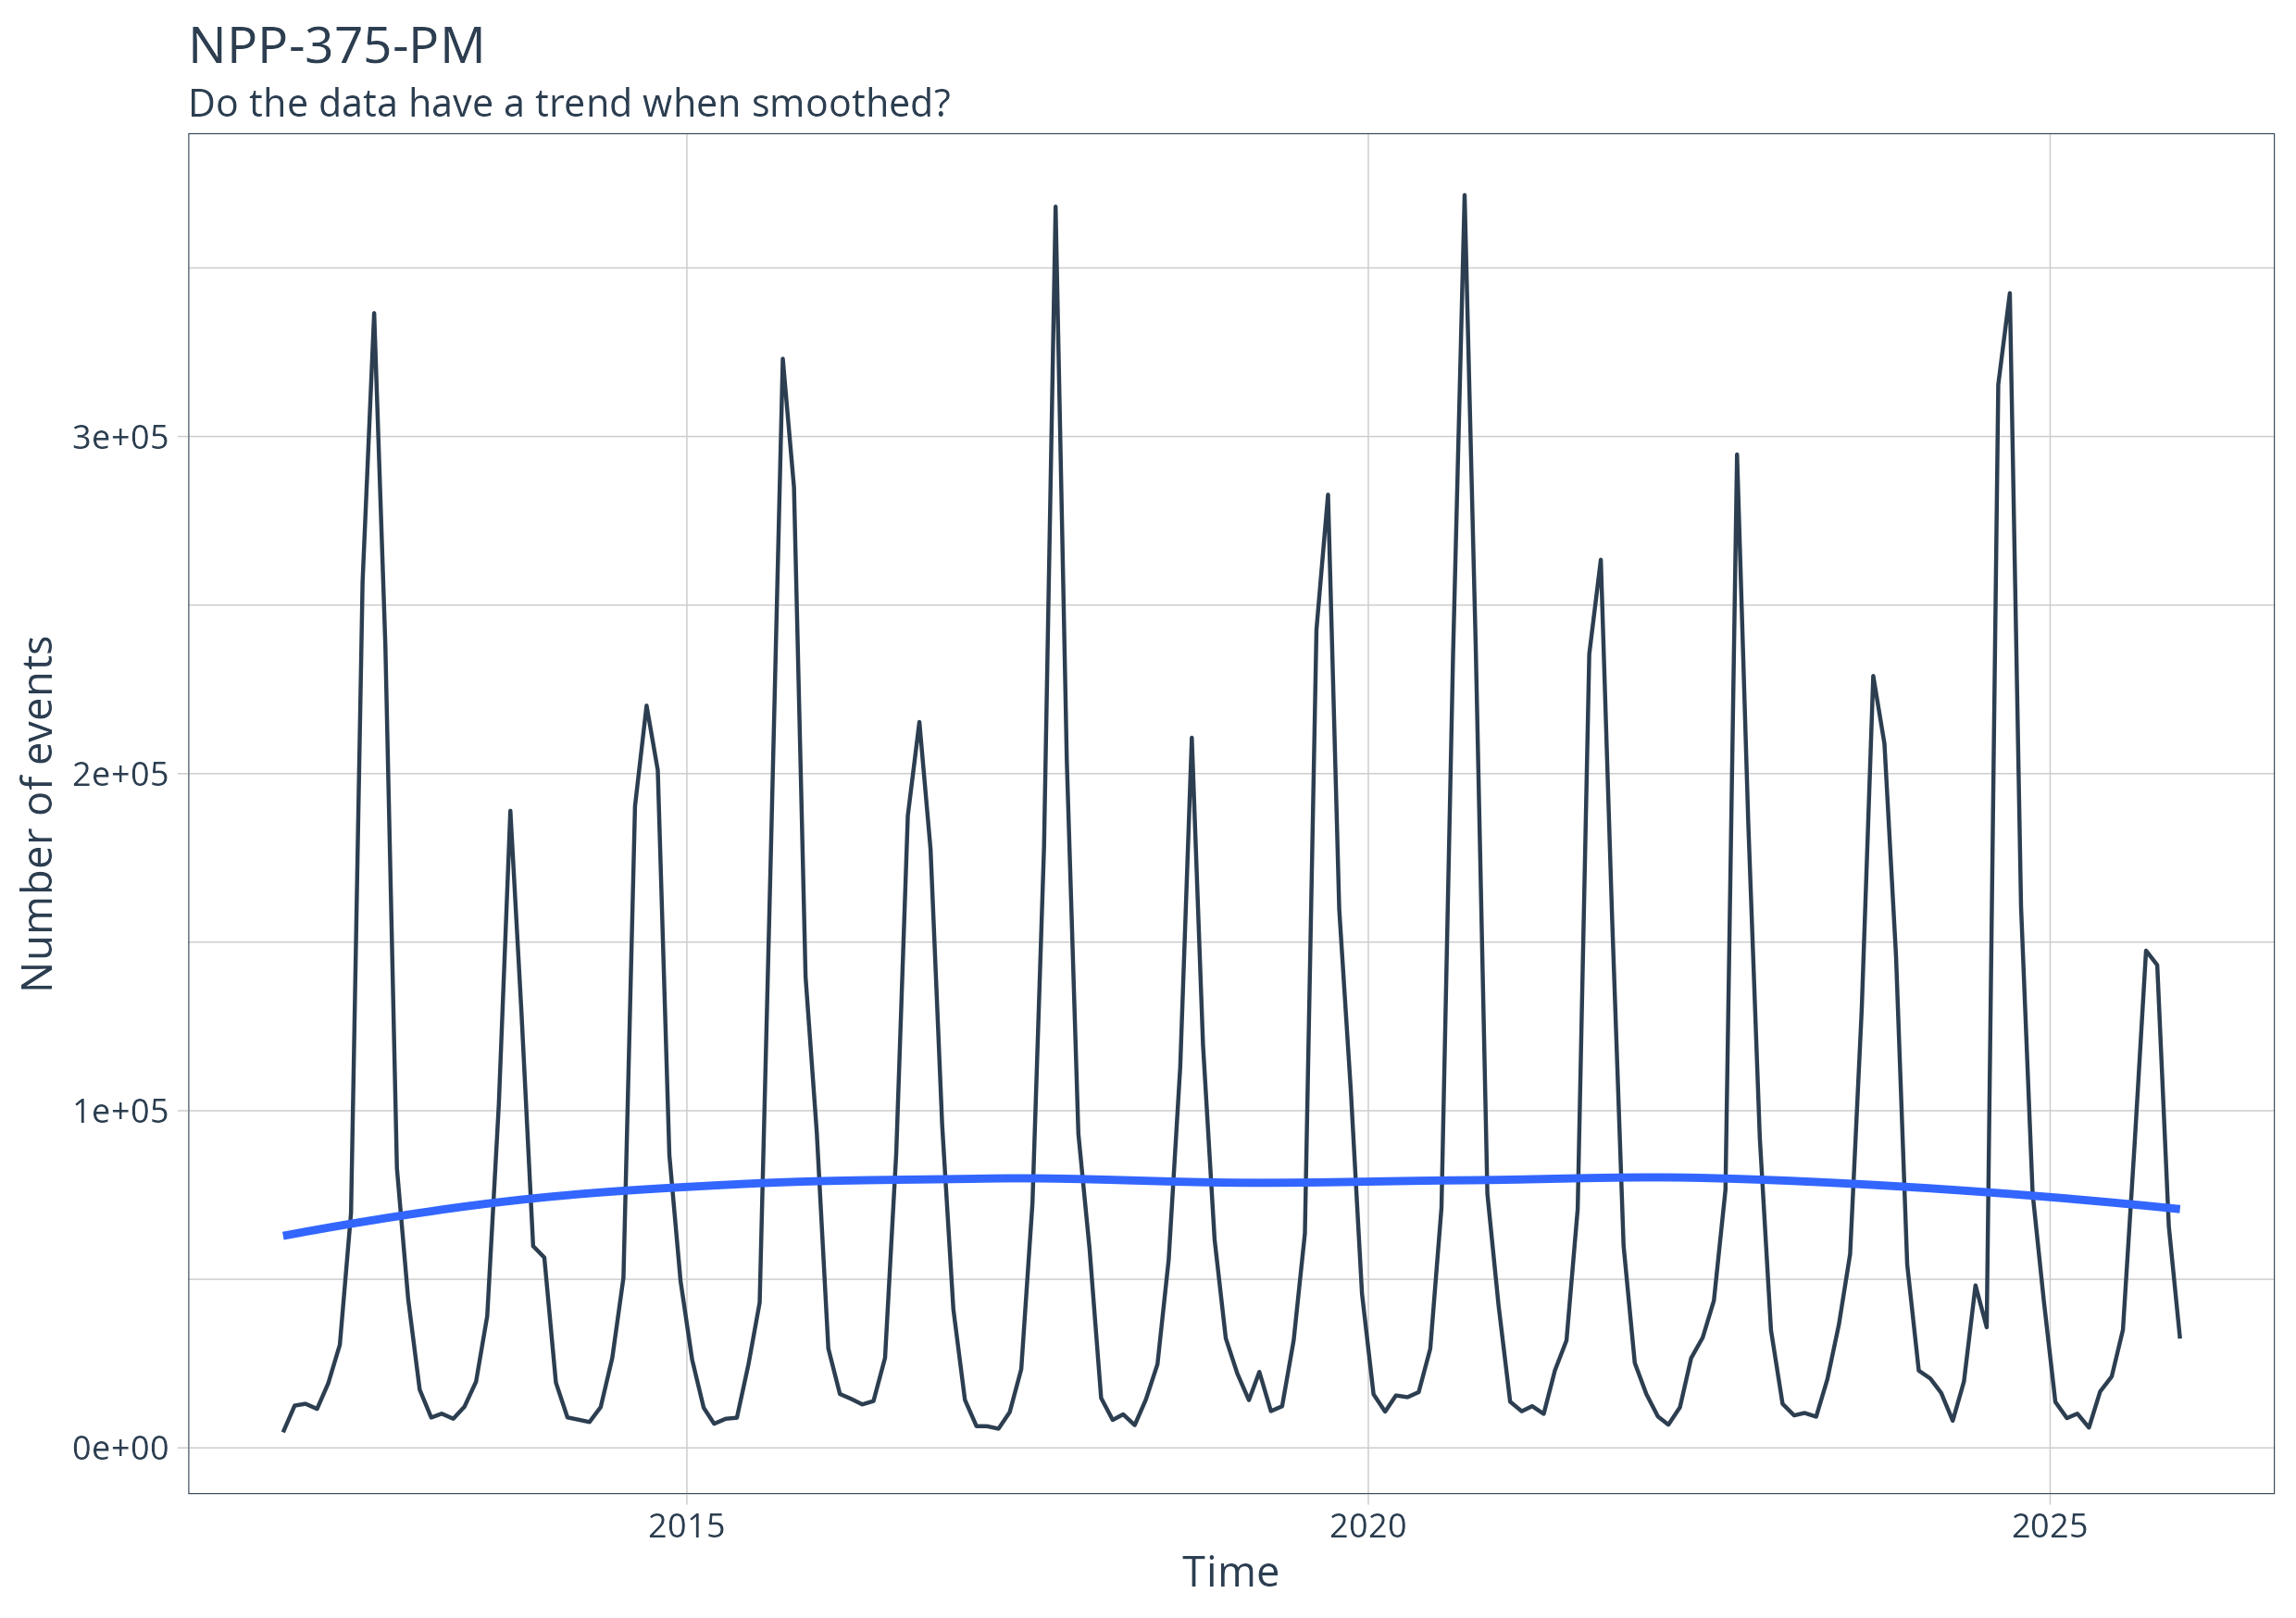
\includegraphics[scale=0.35]{figures/plot_trend_smoothing_NPP-375-PM.png}
    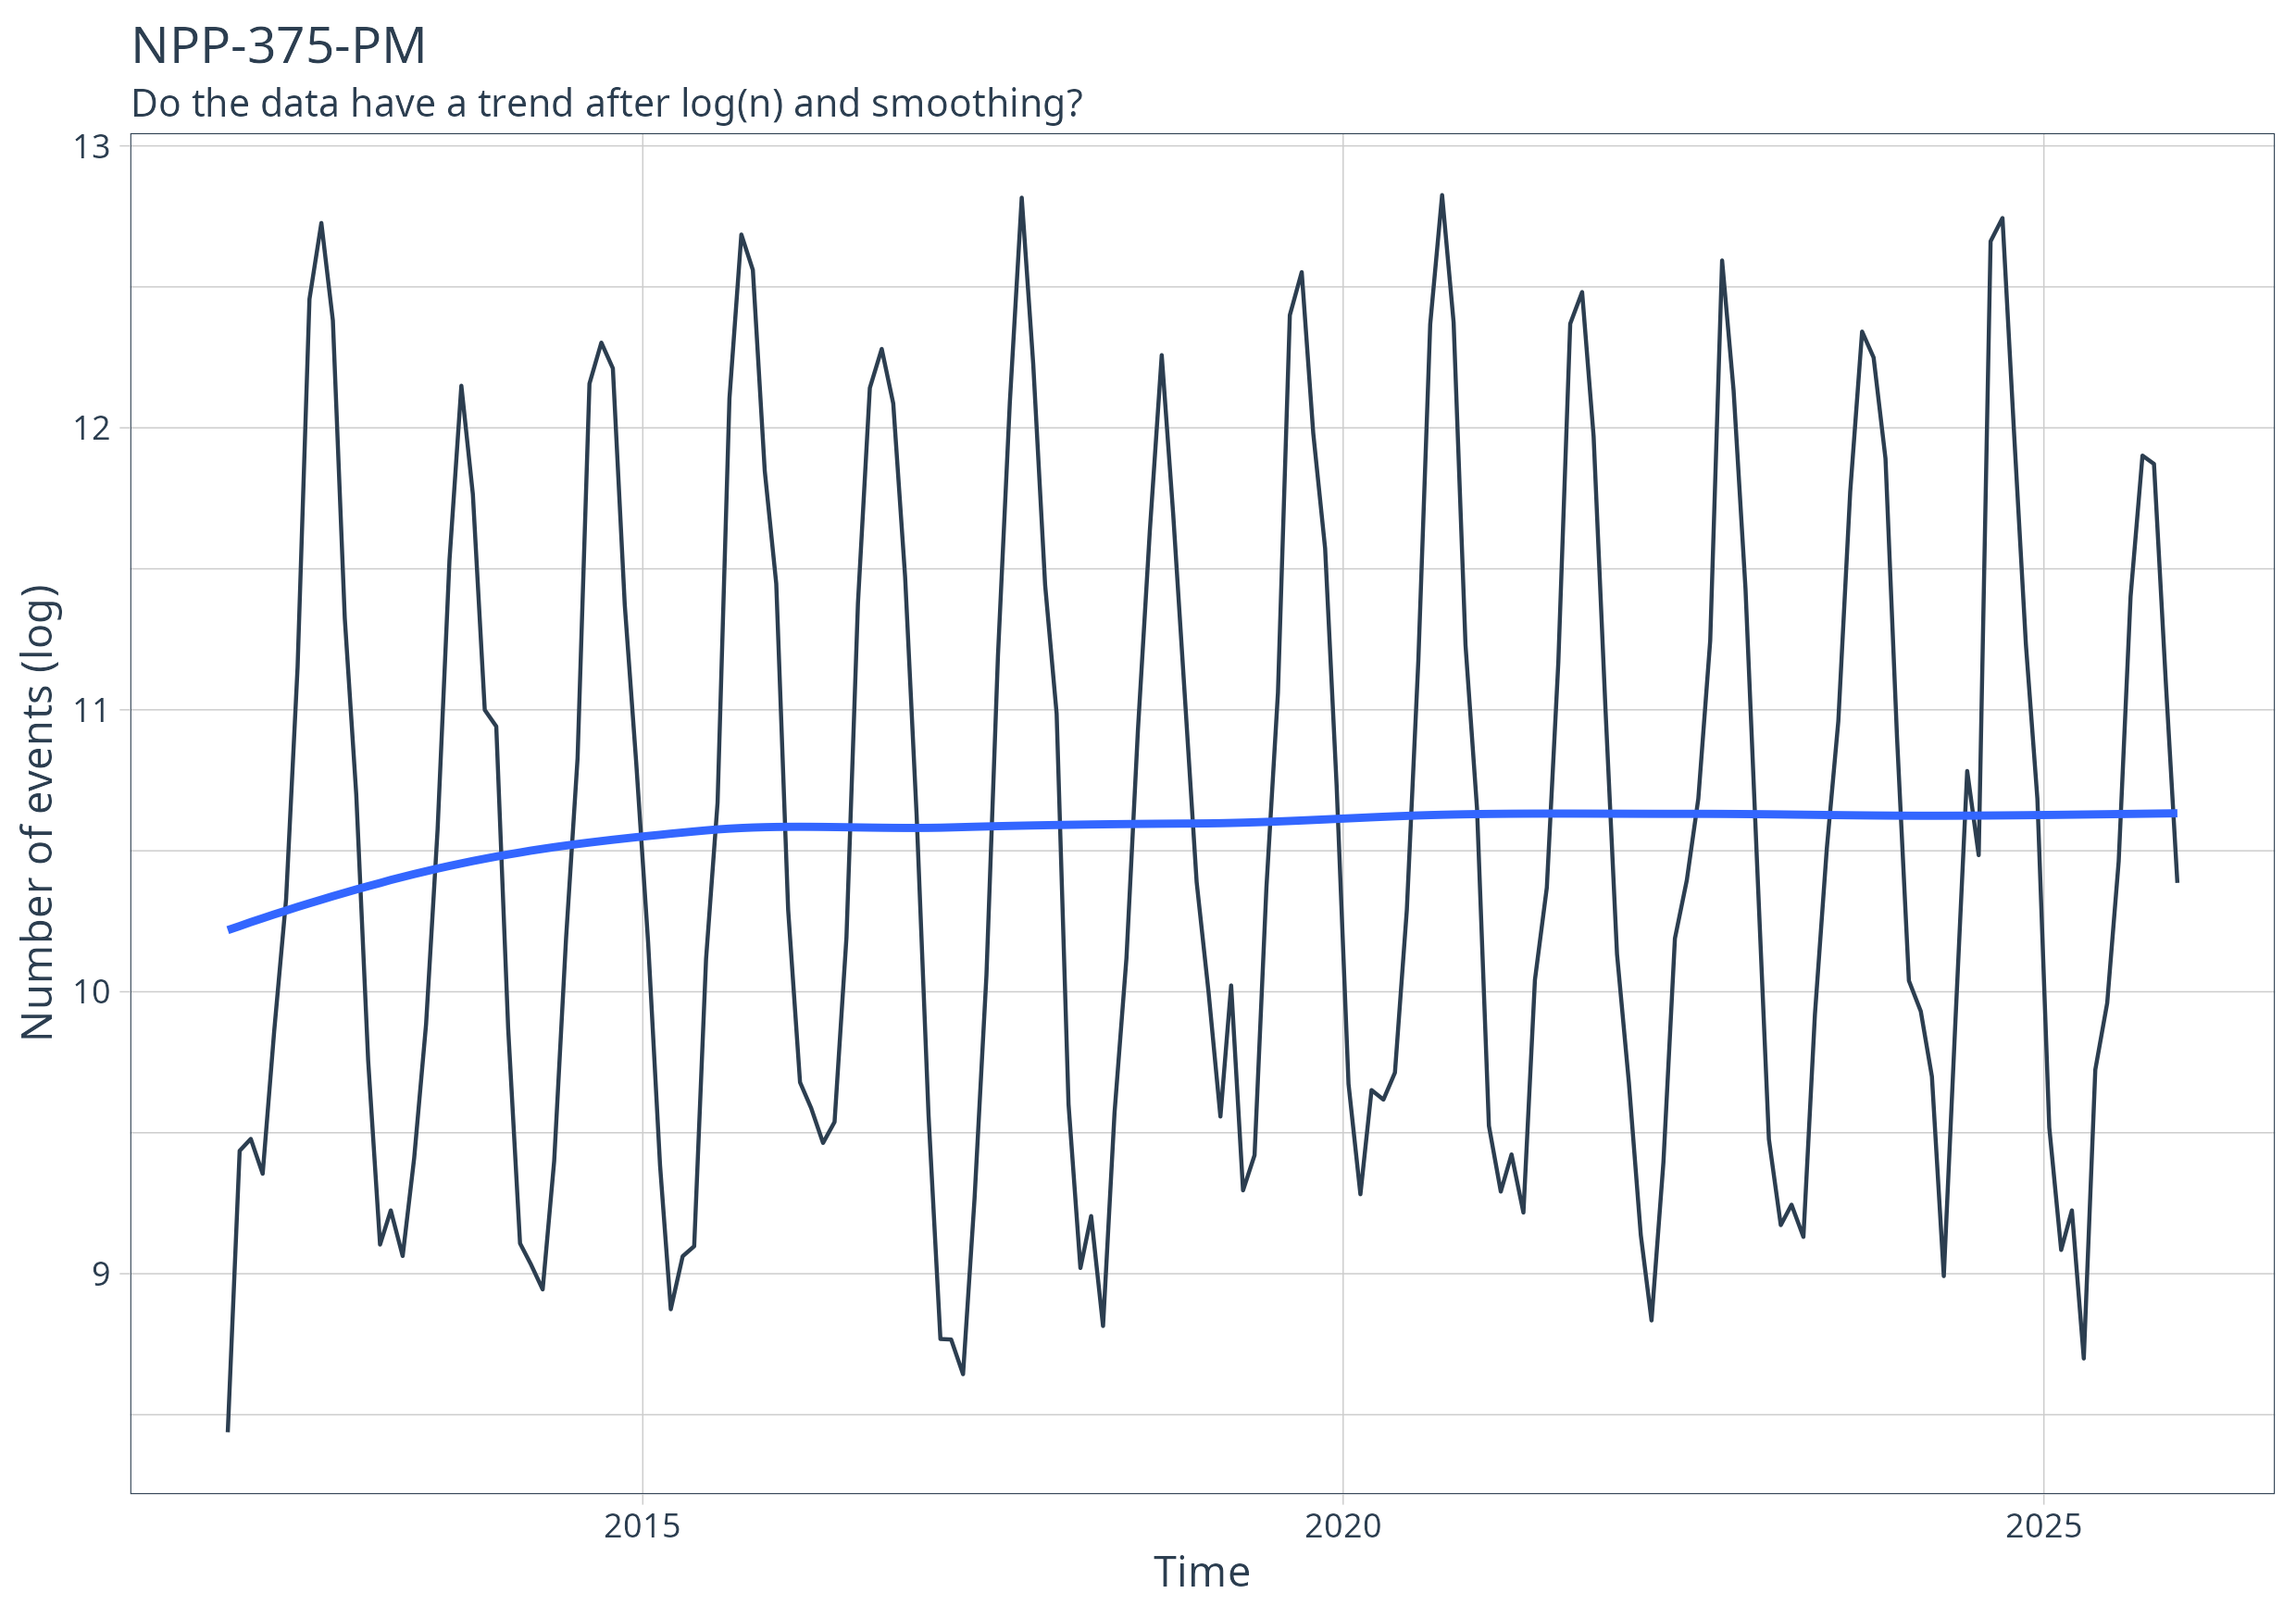
\includegraphics[scale=0.35]{figures/plot_trend_smoothing_log_NPP-375-PM.png}
    \caption{Do the data have a trend when smoothed?}
  \end{figure}
\end{frame}

\begin{frame}
  \frametitle{Time series autocorrelation}
  \begin{figure}
    \centering
    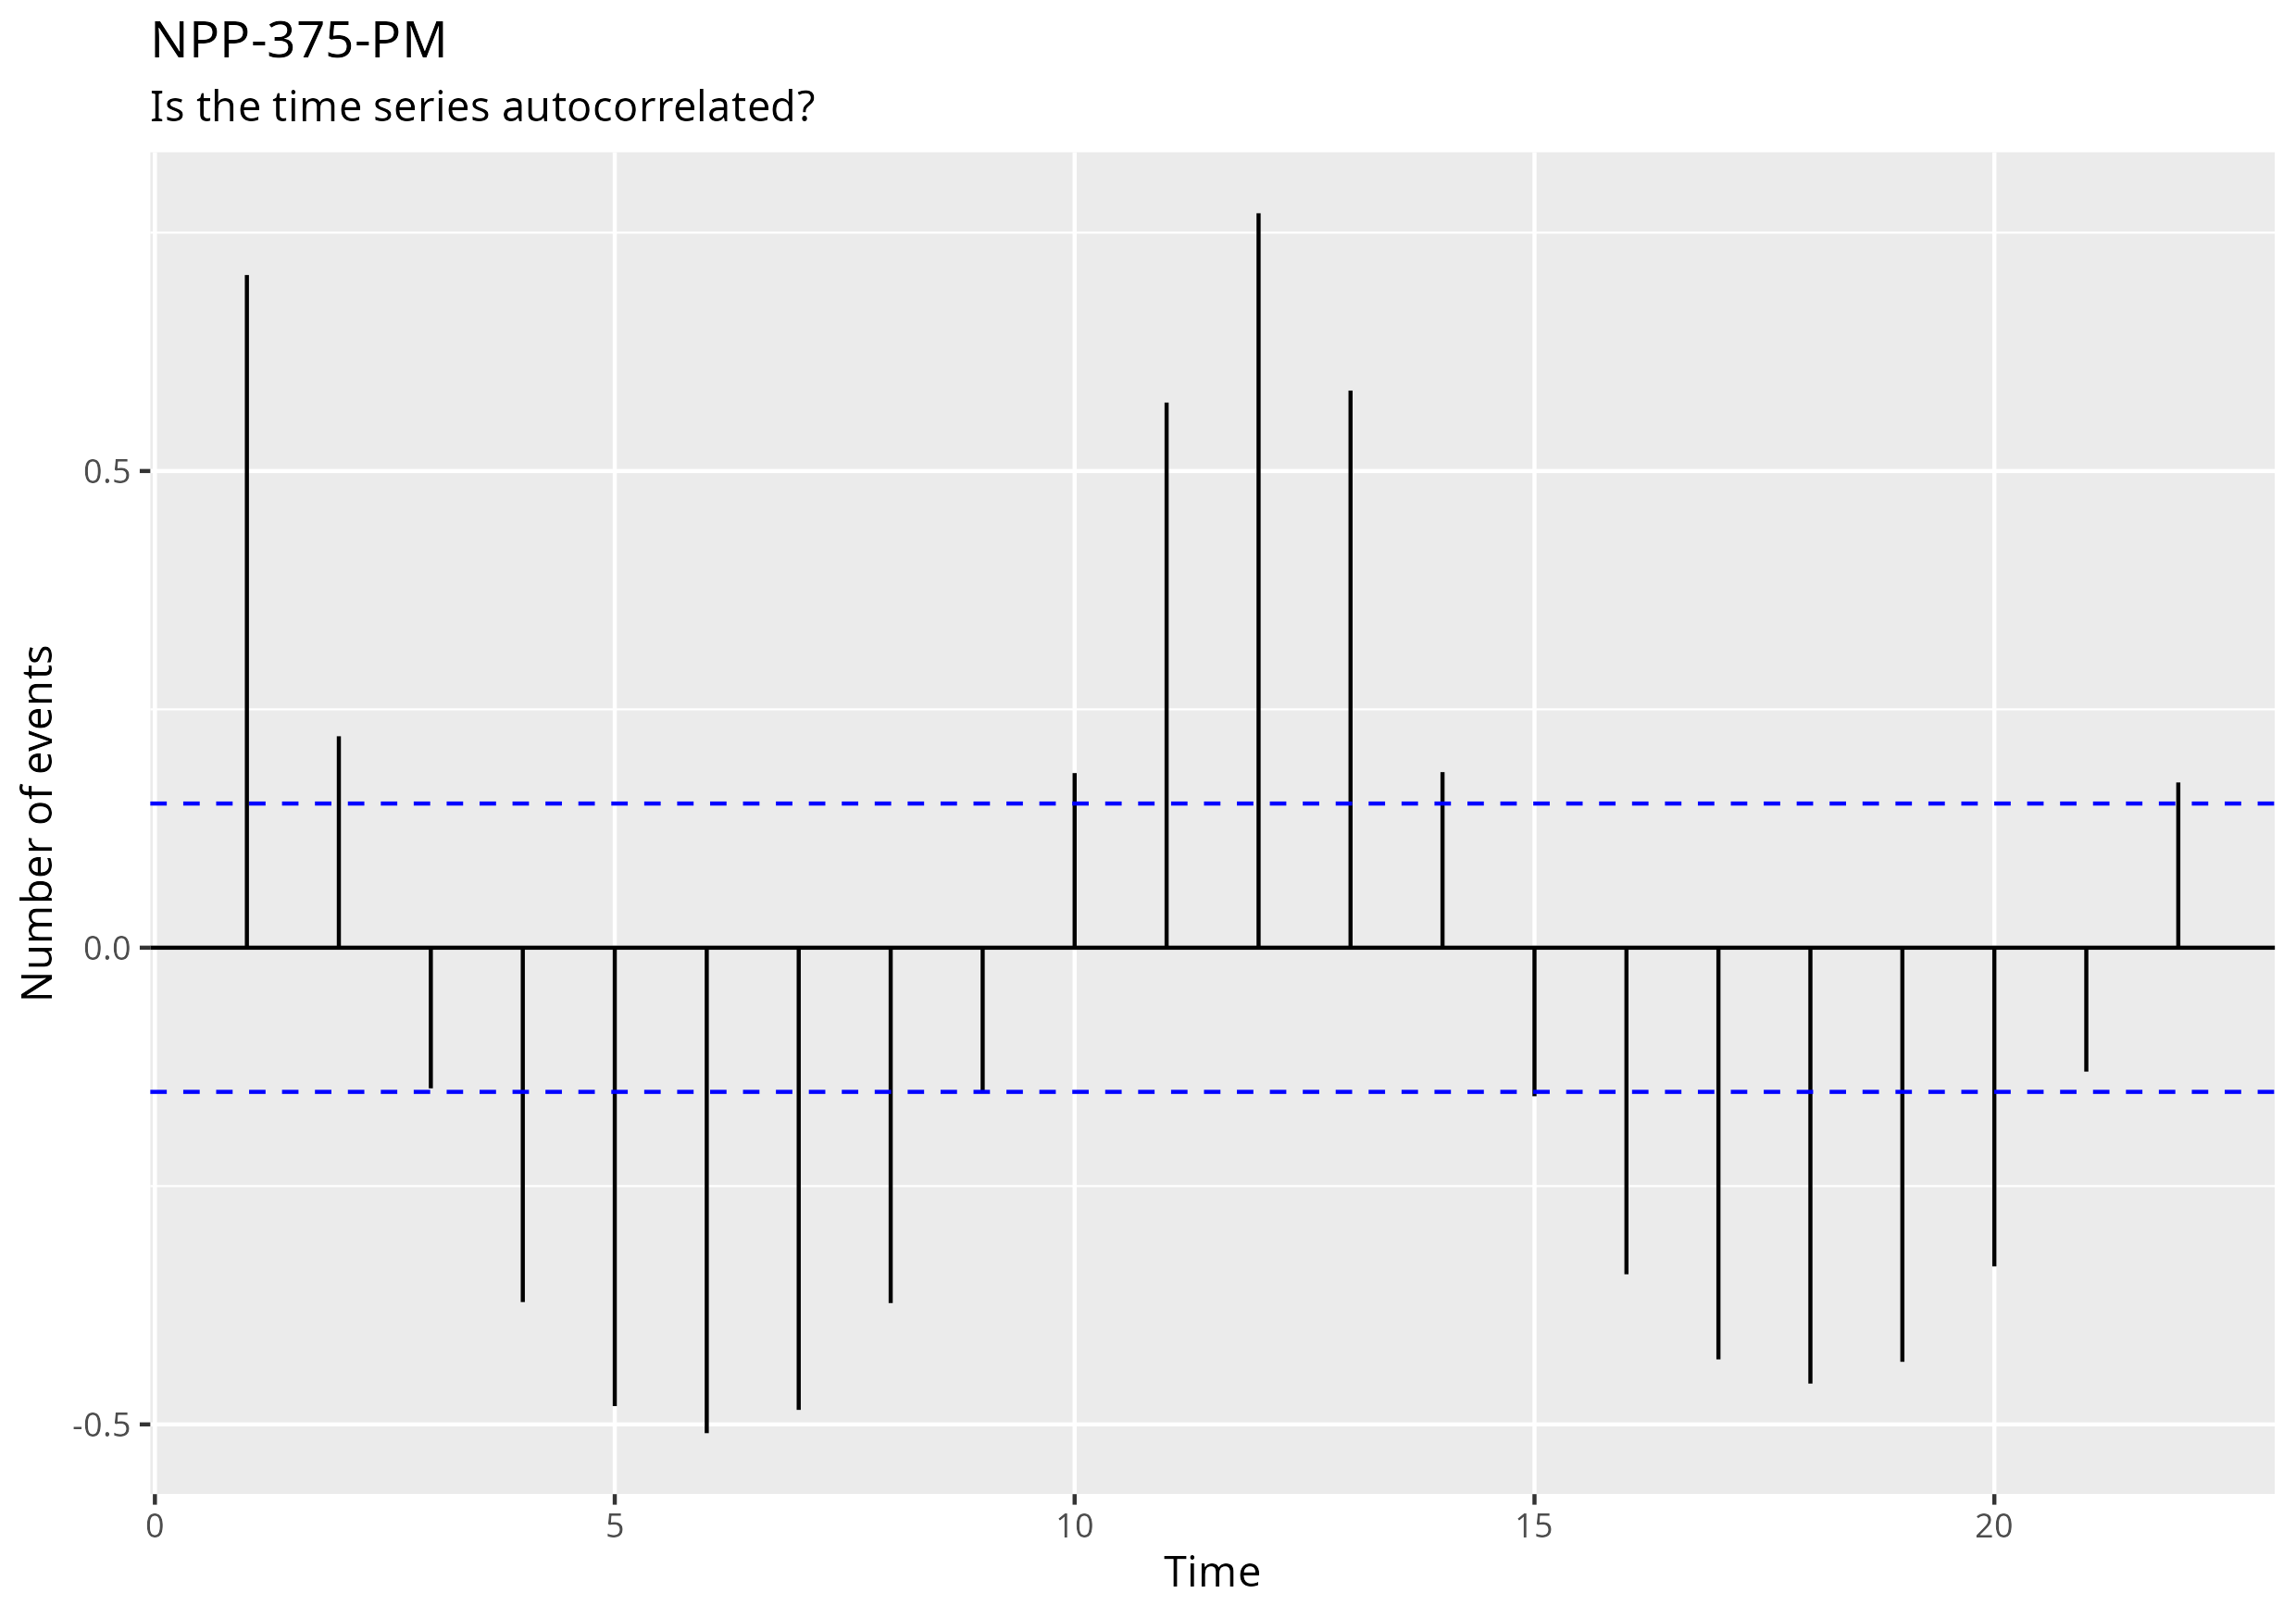
\includegraphics[scale=0.45]{figures/plot_autocorrelation_NPP-375-PM.png}
    \caption{Is the time series autocorrelated?}
  \end{figure}
\end{frame}

\begin{frame}
  \frametitle{Time series trend}
  \begin{figure}
    \centering
    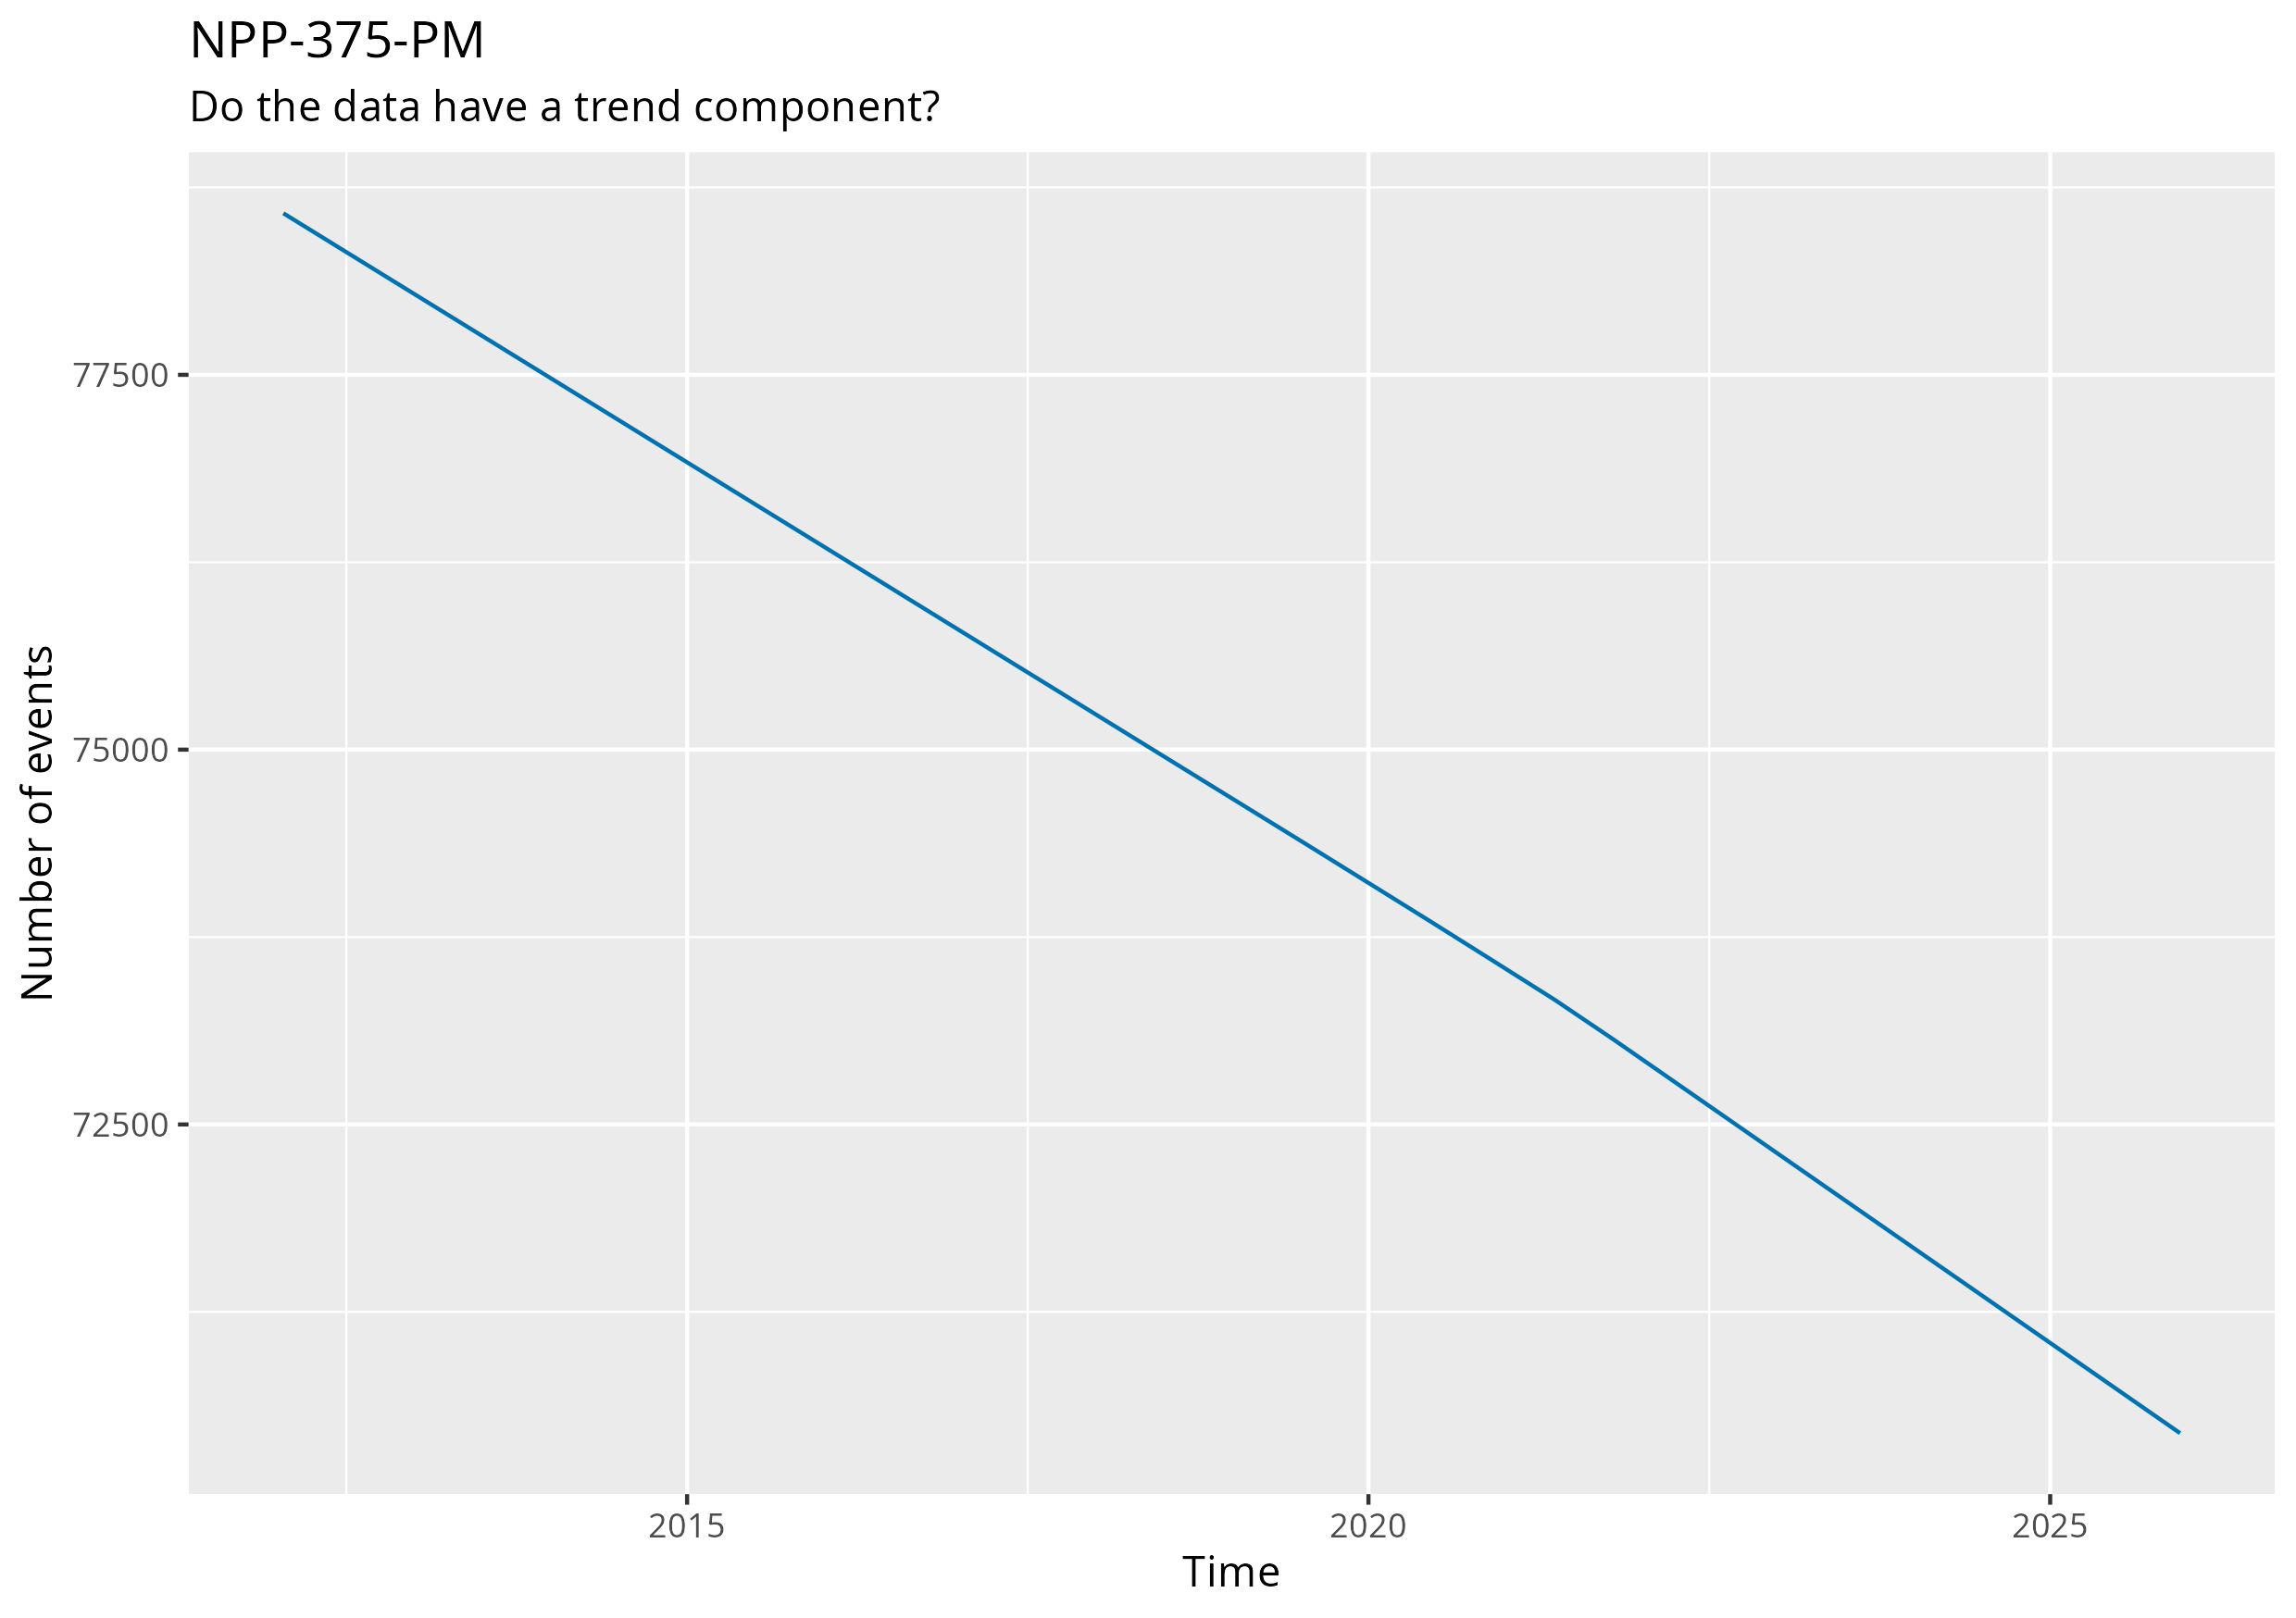
\includegraphics[scale=0.5]{figures/plot_component_trend_NPP-375-PM.png}
    \caption{Do the data have a trend component?}
  \end{figure}
\end{frame}

\begin{frame}
  \frametitle{Time series seasonality}
  \begin{figure}
    \centering
    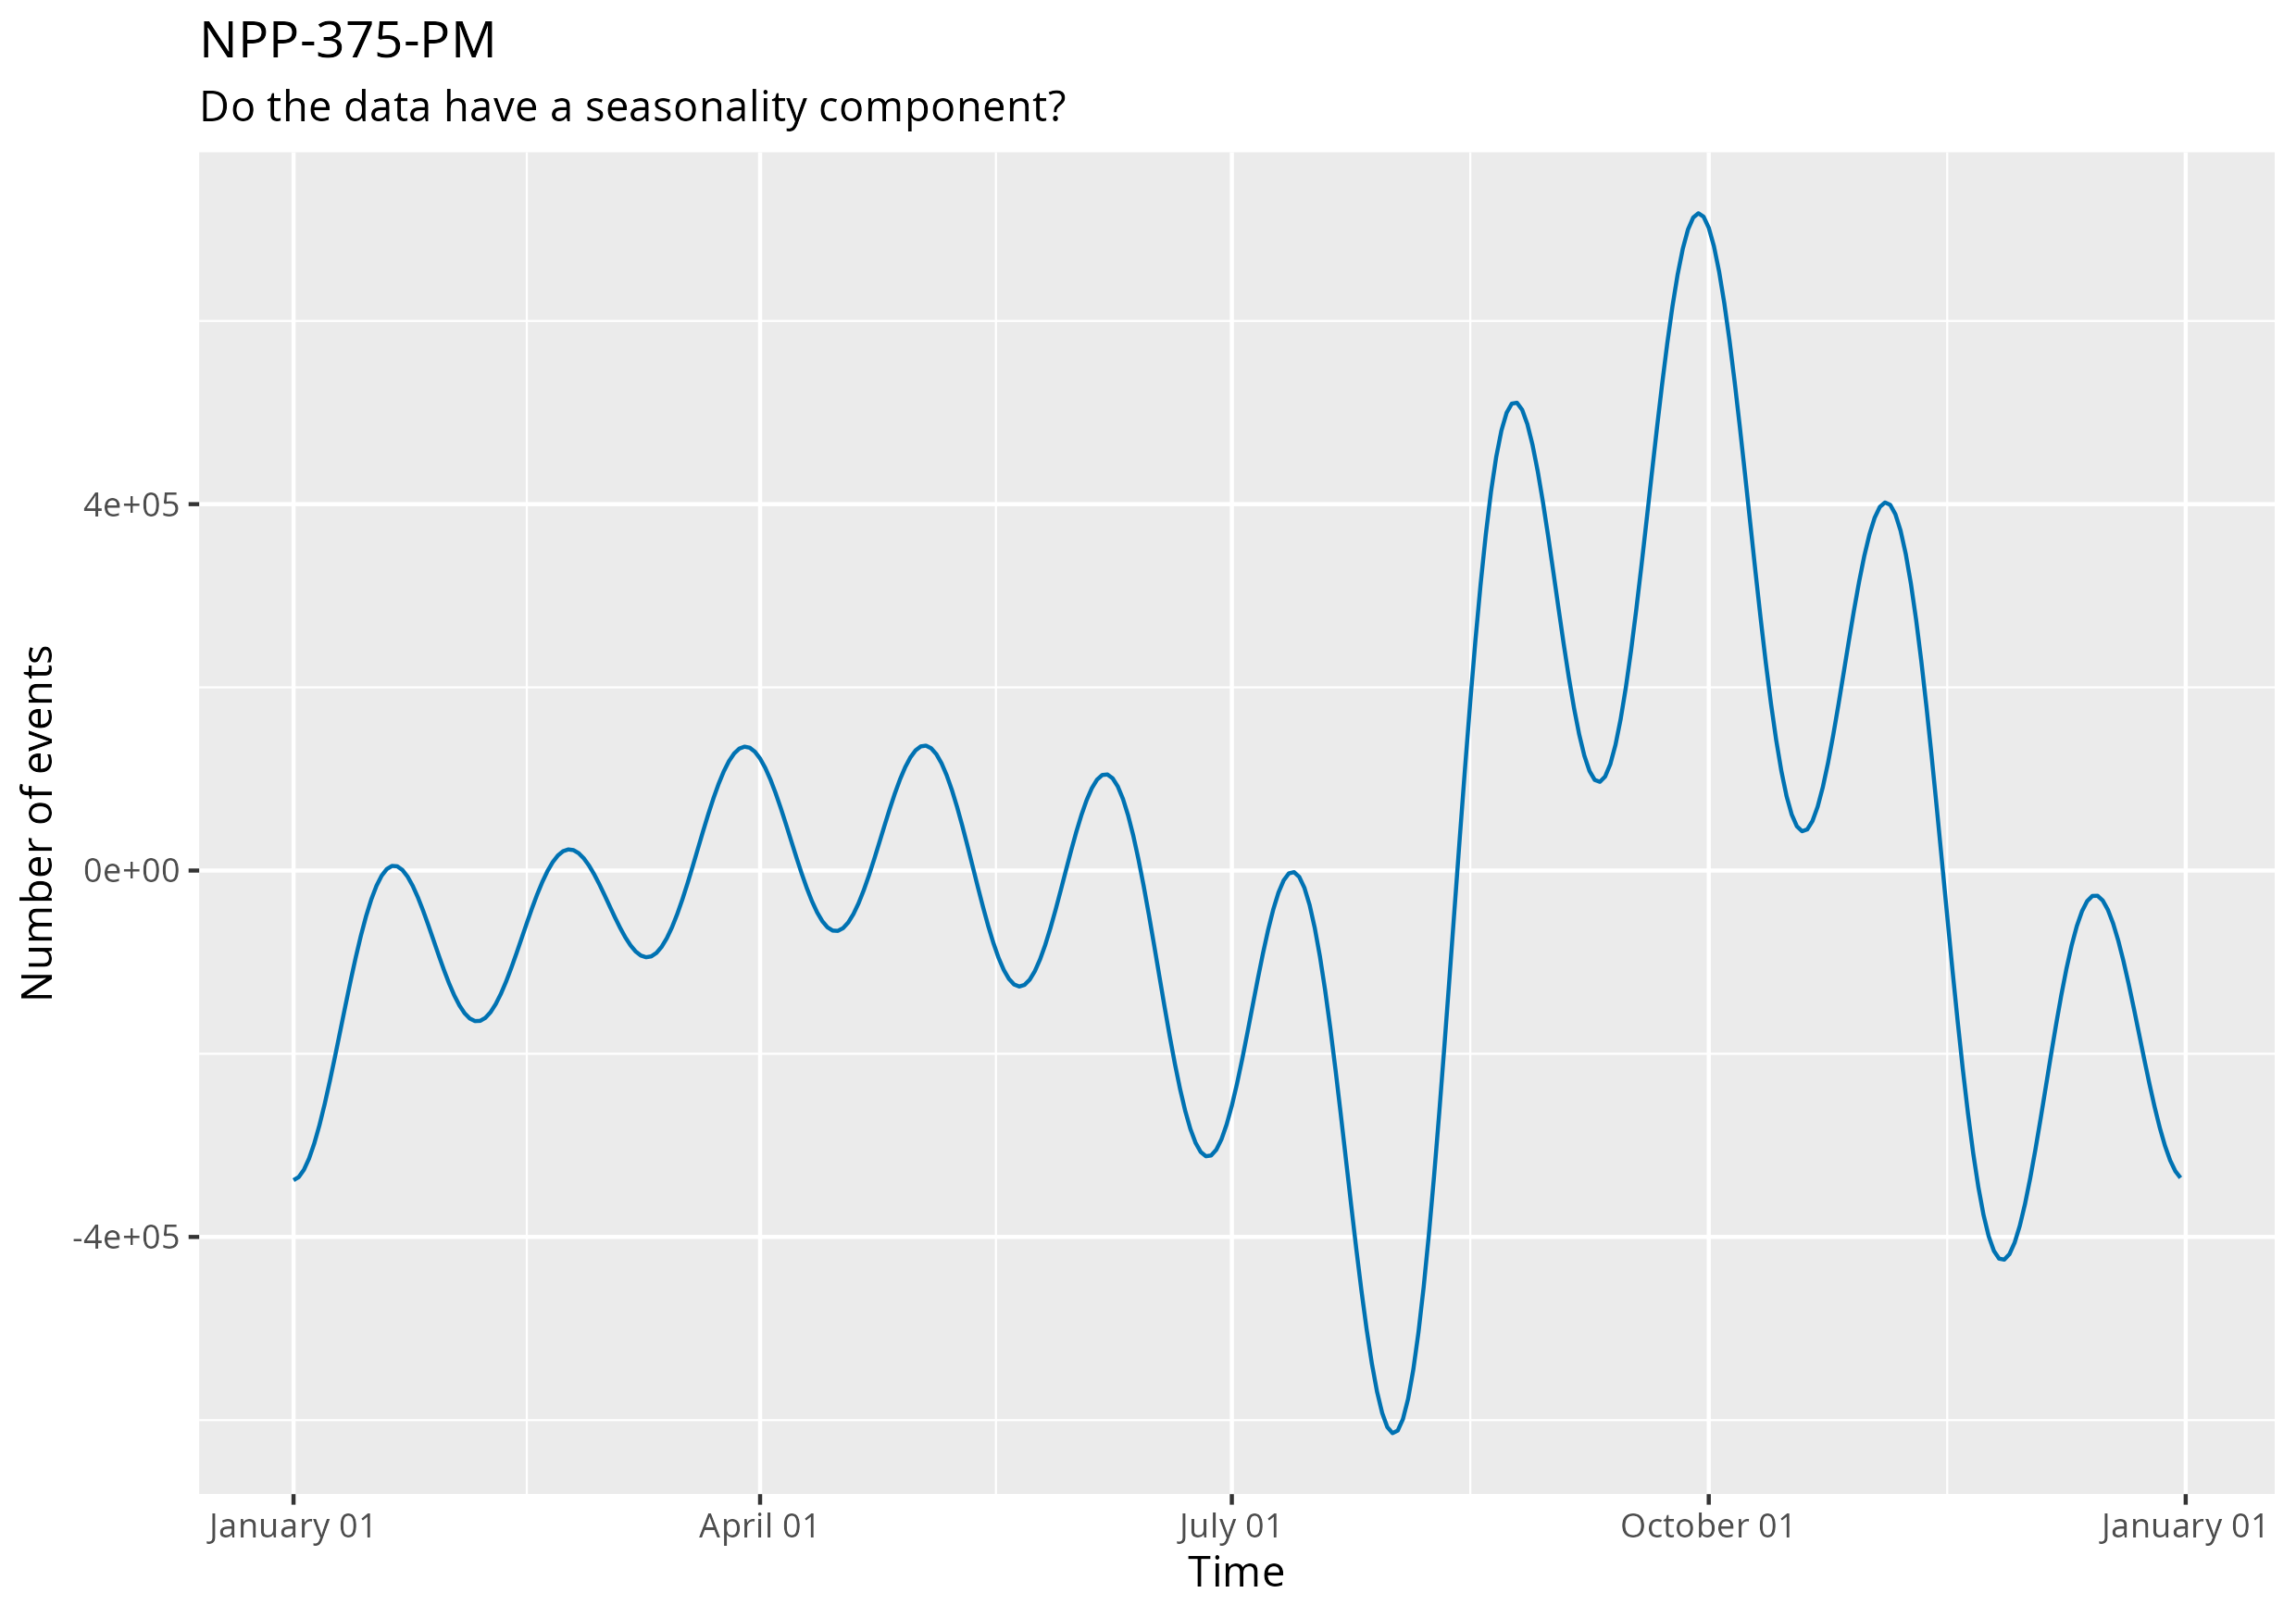
\includegraphics[scale=0.5]{figures/plot_component_seasonality_NPP-375-PM.png}
    \caption{Do the data have a seasonality component?}
  \end{figure}
\end{frame}

\begin{frame}
  \frametitle{Time series versus forecast}
  \begin{figure}
    \centering
    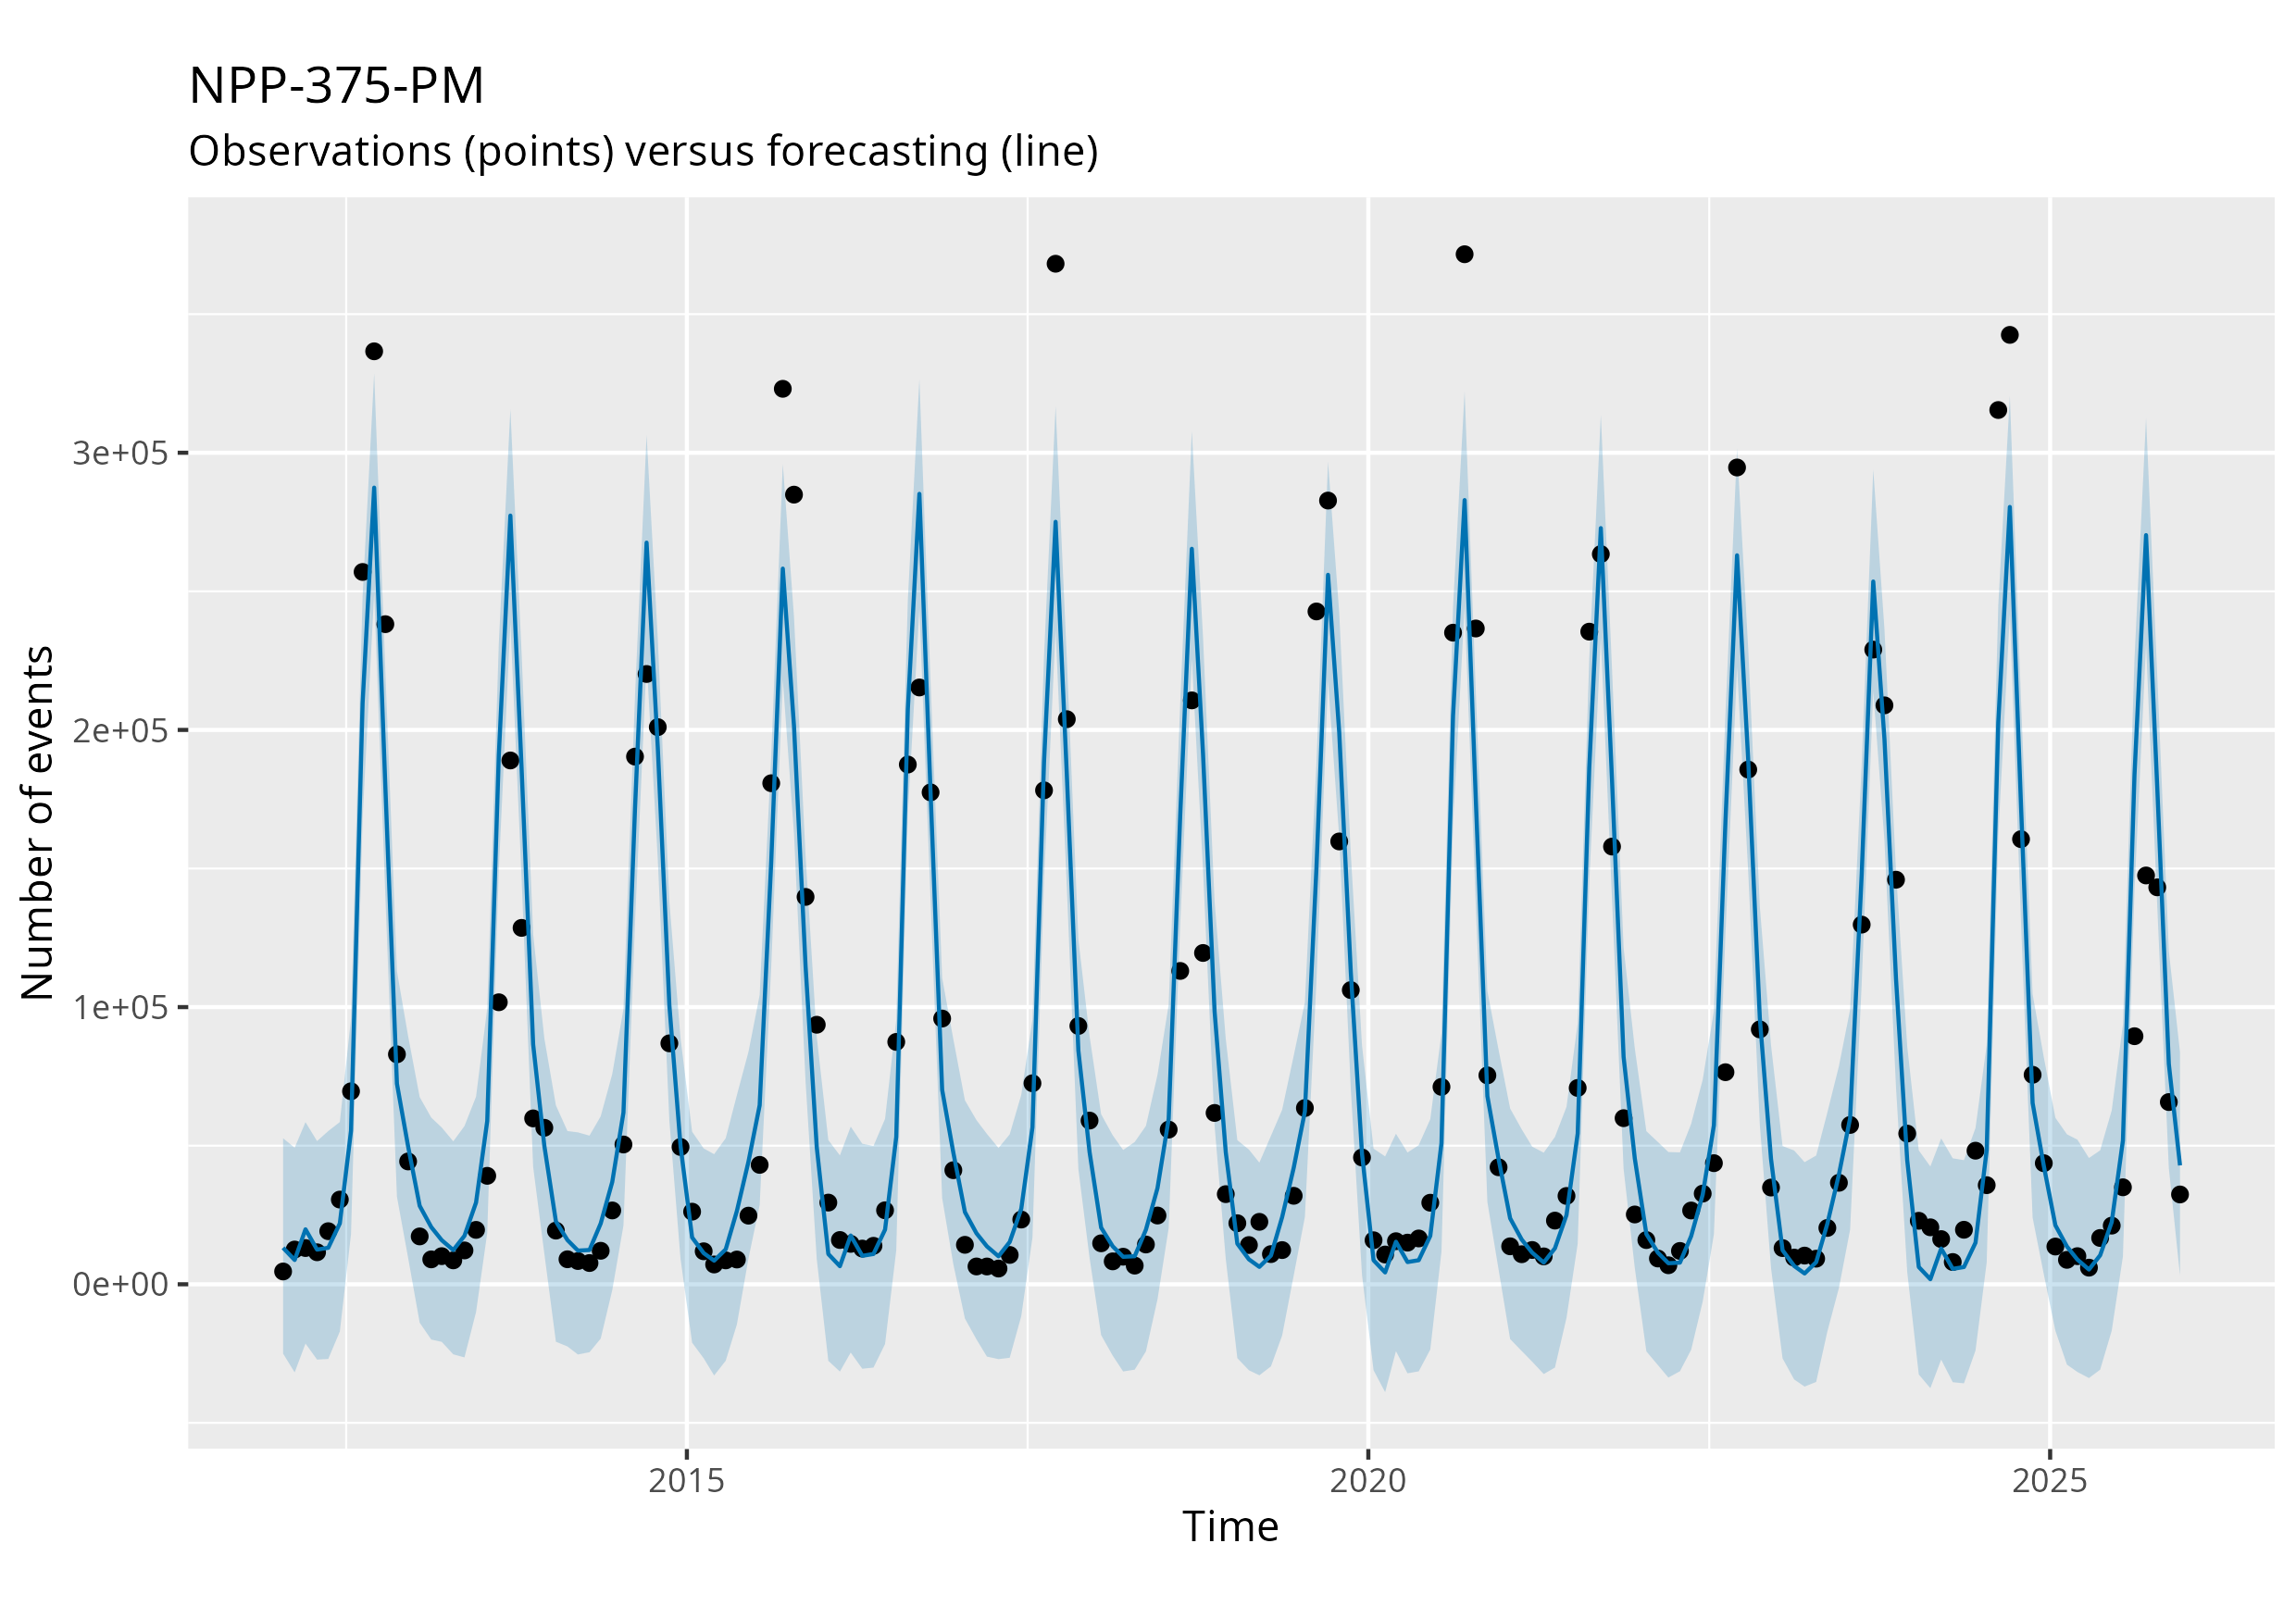
\includegraphics[scale=0.45]{figures/plot_model_forecast_NPP-375-PM.png}
    \caption{Observations (black dots) and model (blue line) with a confidence
    interval of 95\% (gray shadow).}
  \end{figure}
\end{frame}

\begin{frame}
  \frametitle{Time series versus forecast}
  \begin{figure}
    \centering
    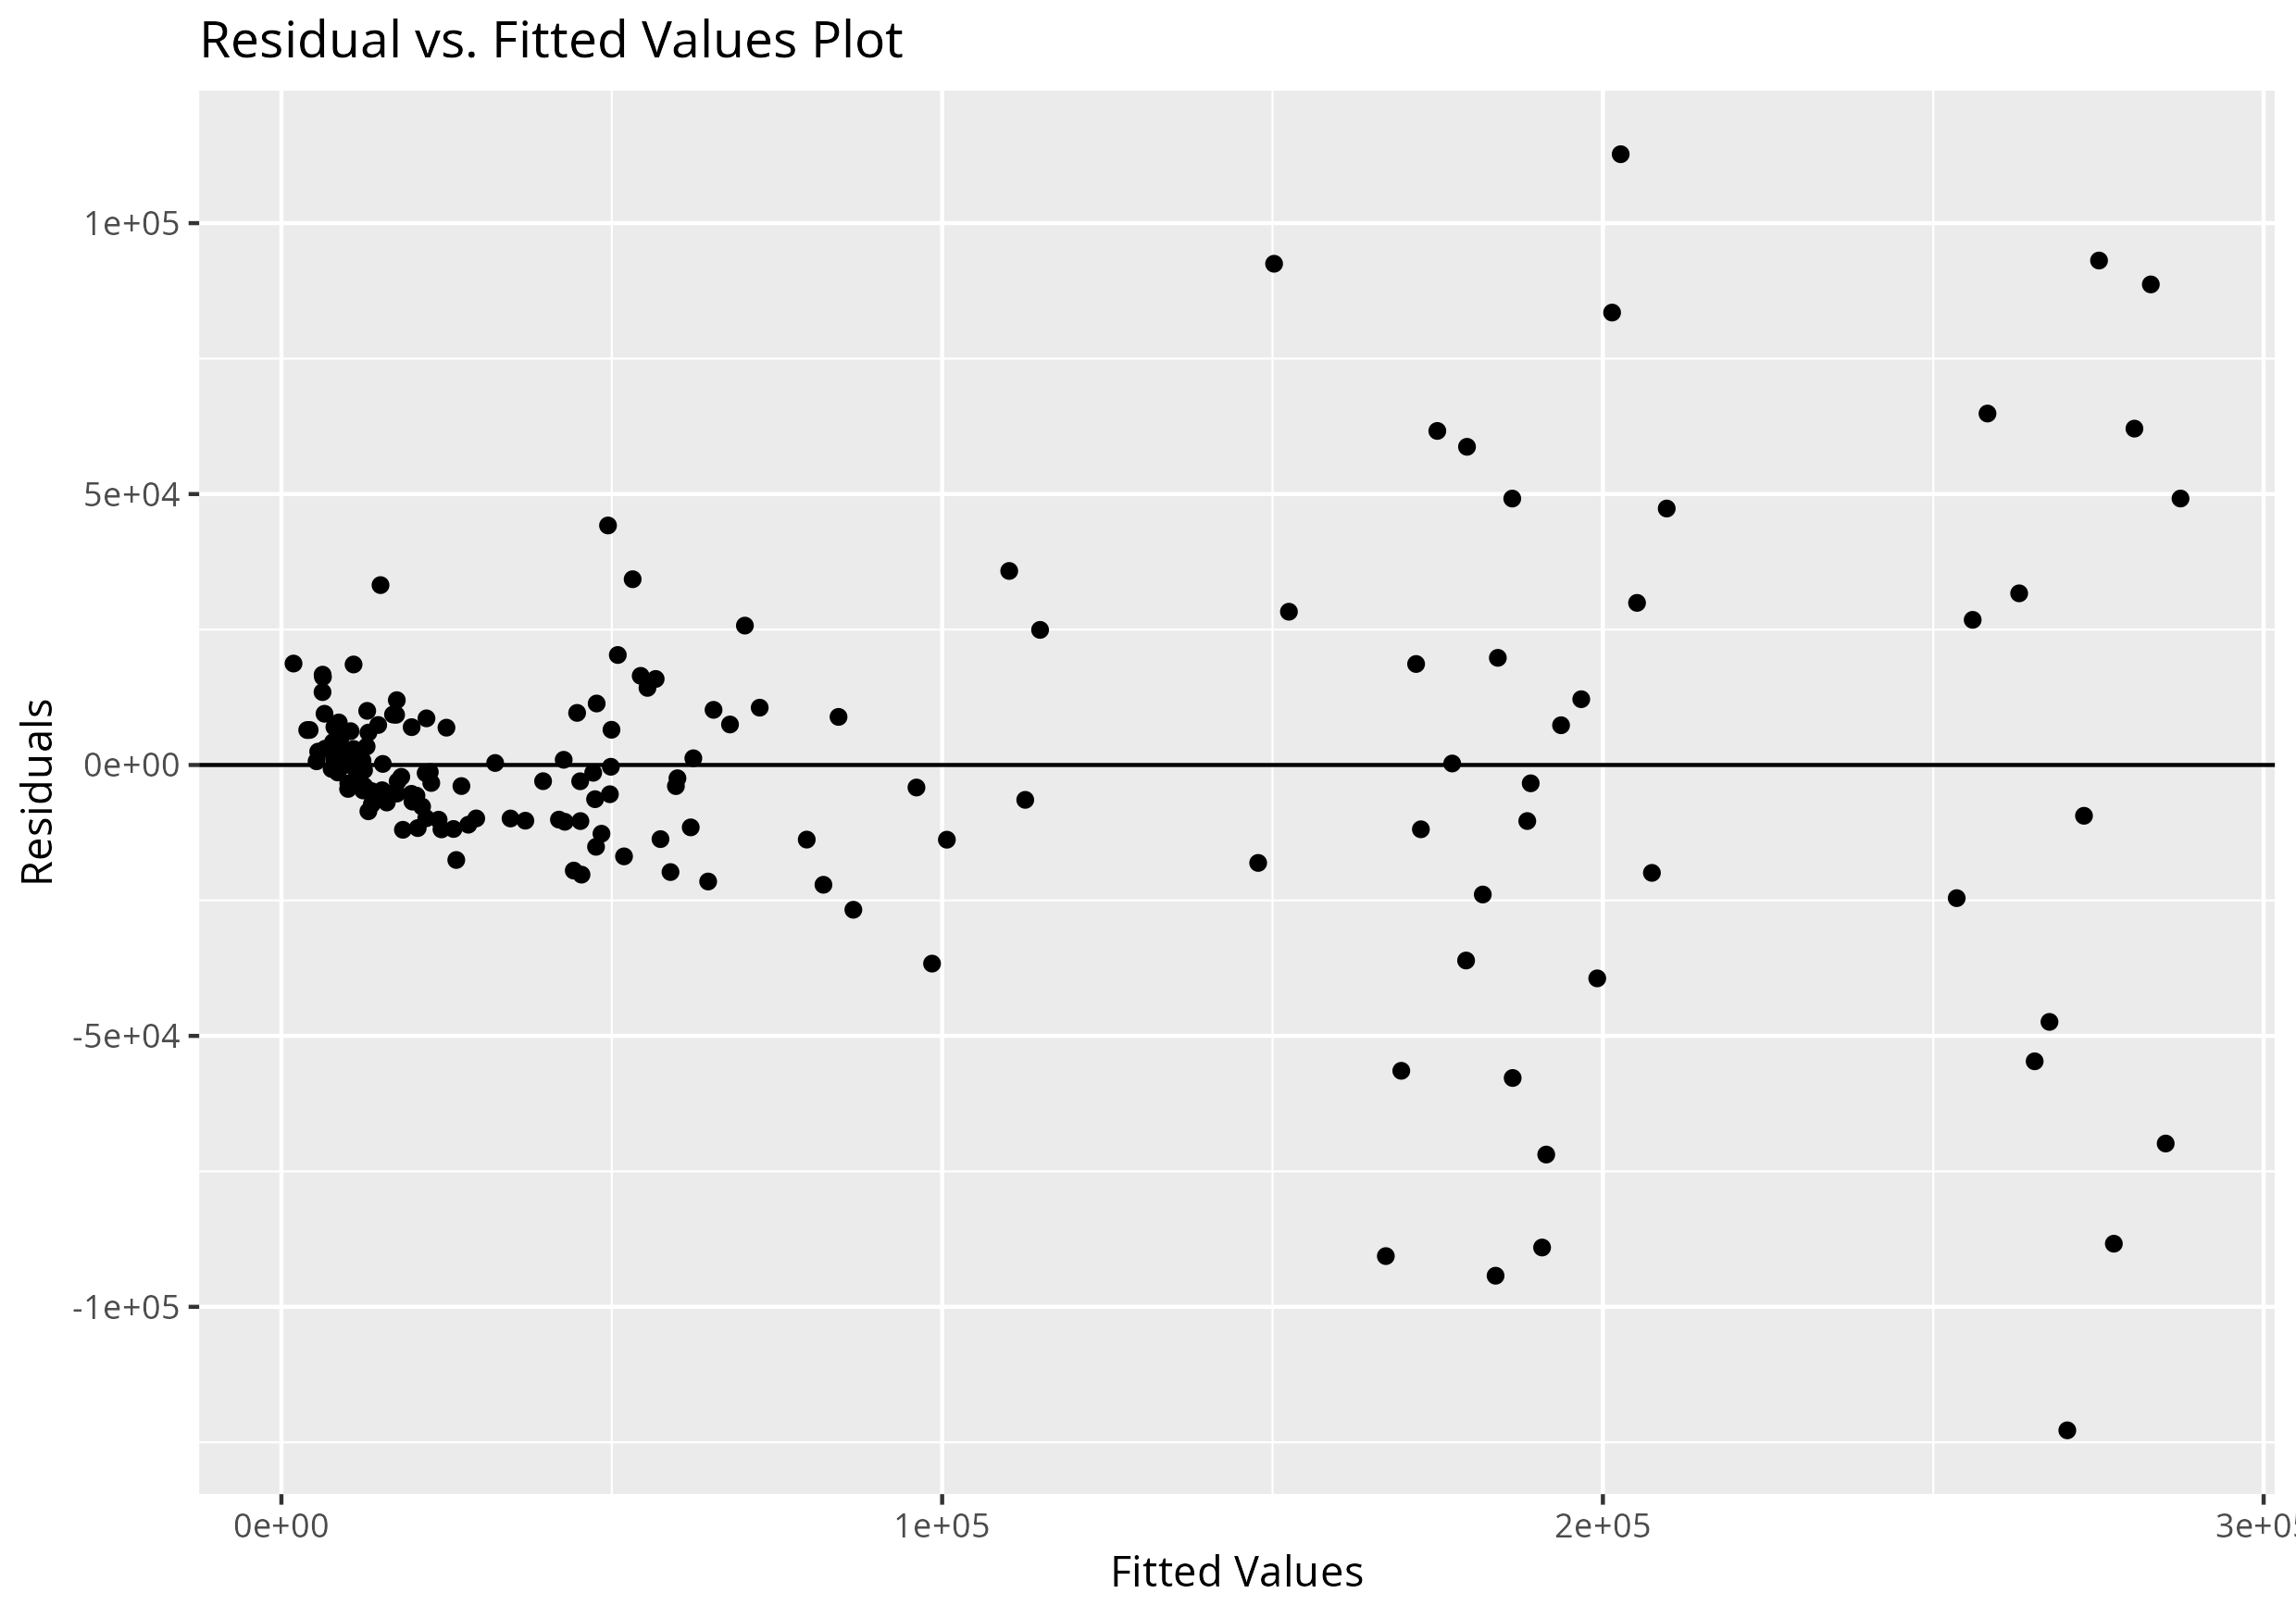
\includegraphics[scale=0.5]{figures/plot_residuals_NPP-375-PM.png}
    \caption{Larger fire foci values have larger residuals.}
  \end{figure}
\end{frame}

\begin{frame}
  \frametitle{Time series versus forecast}
  \begin{figure}
    \centering
    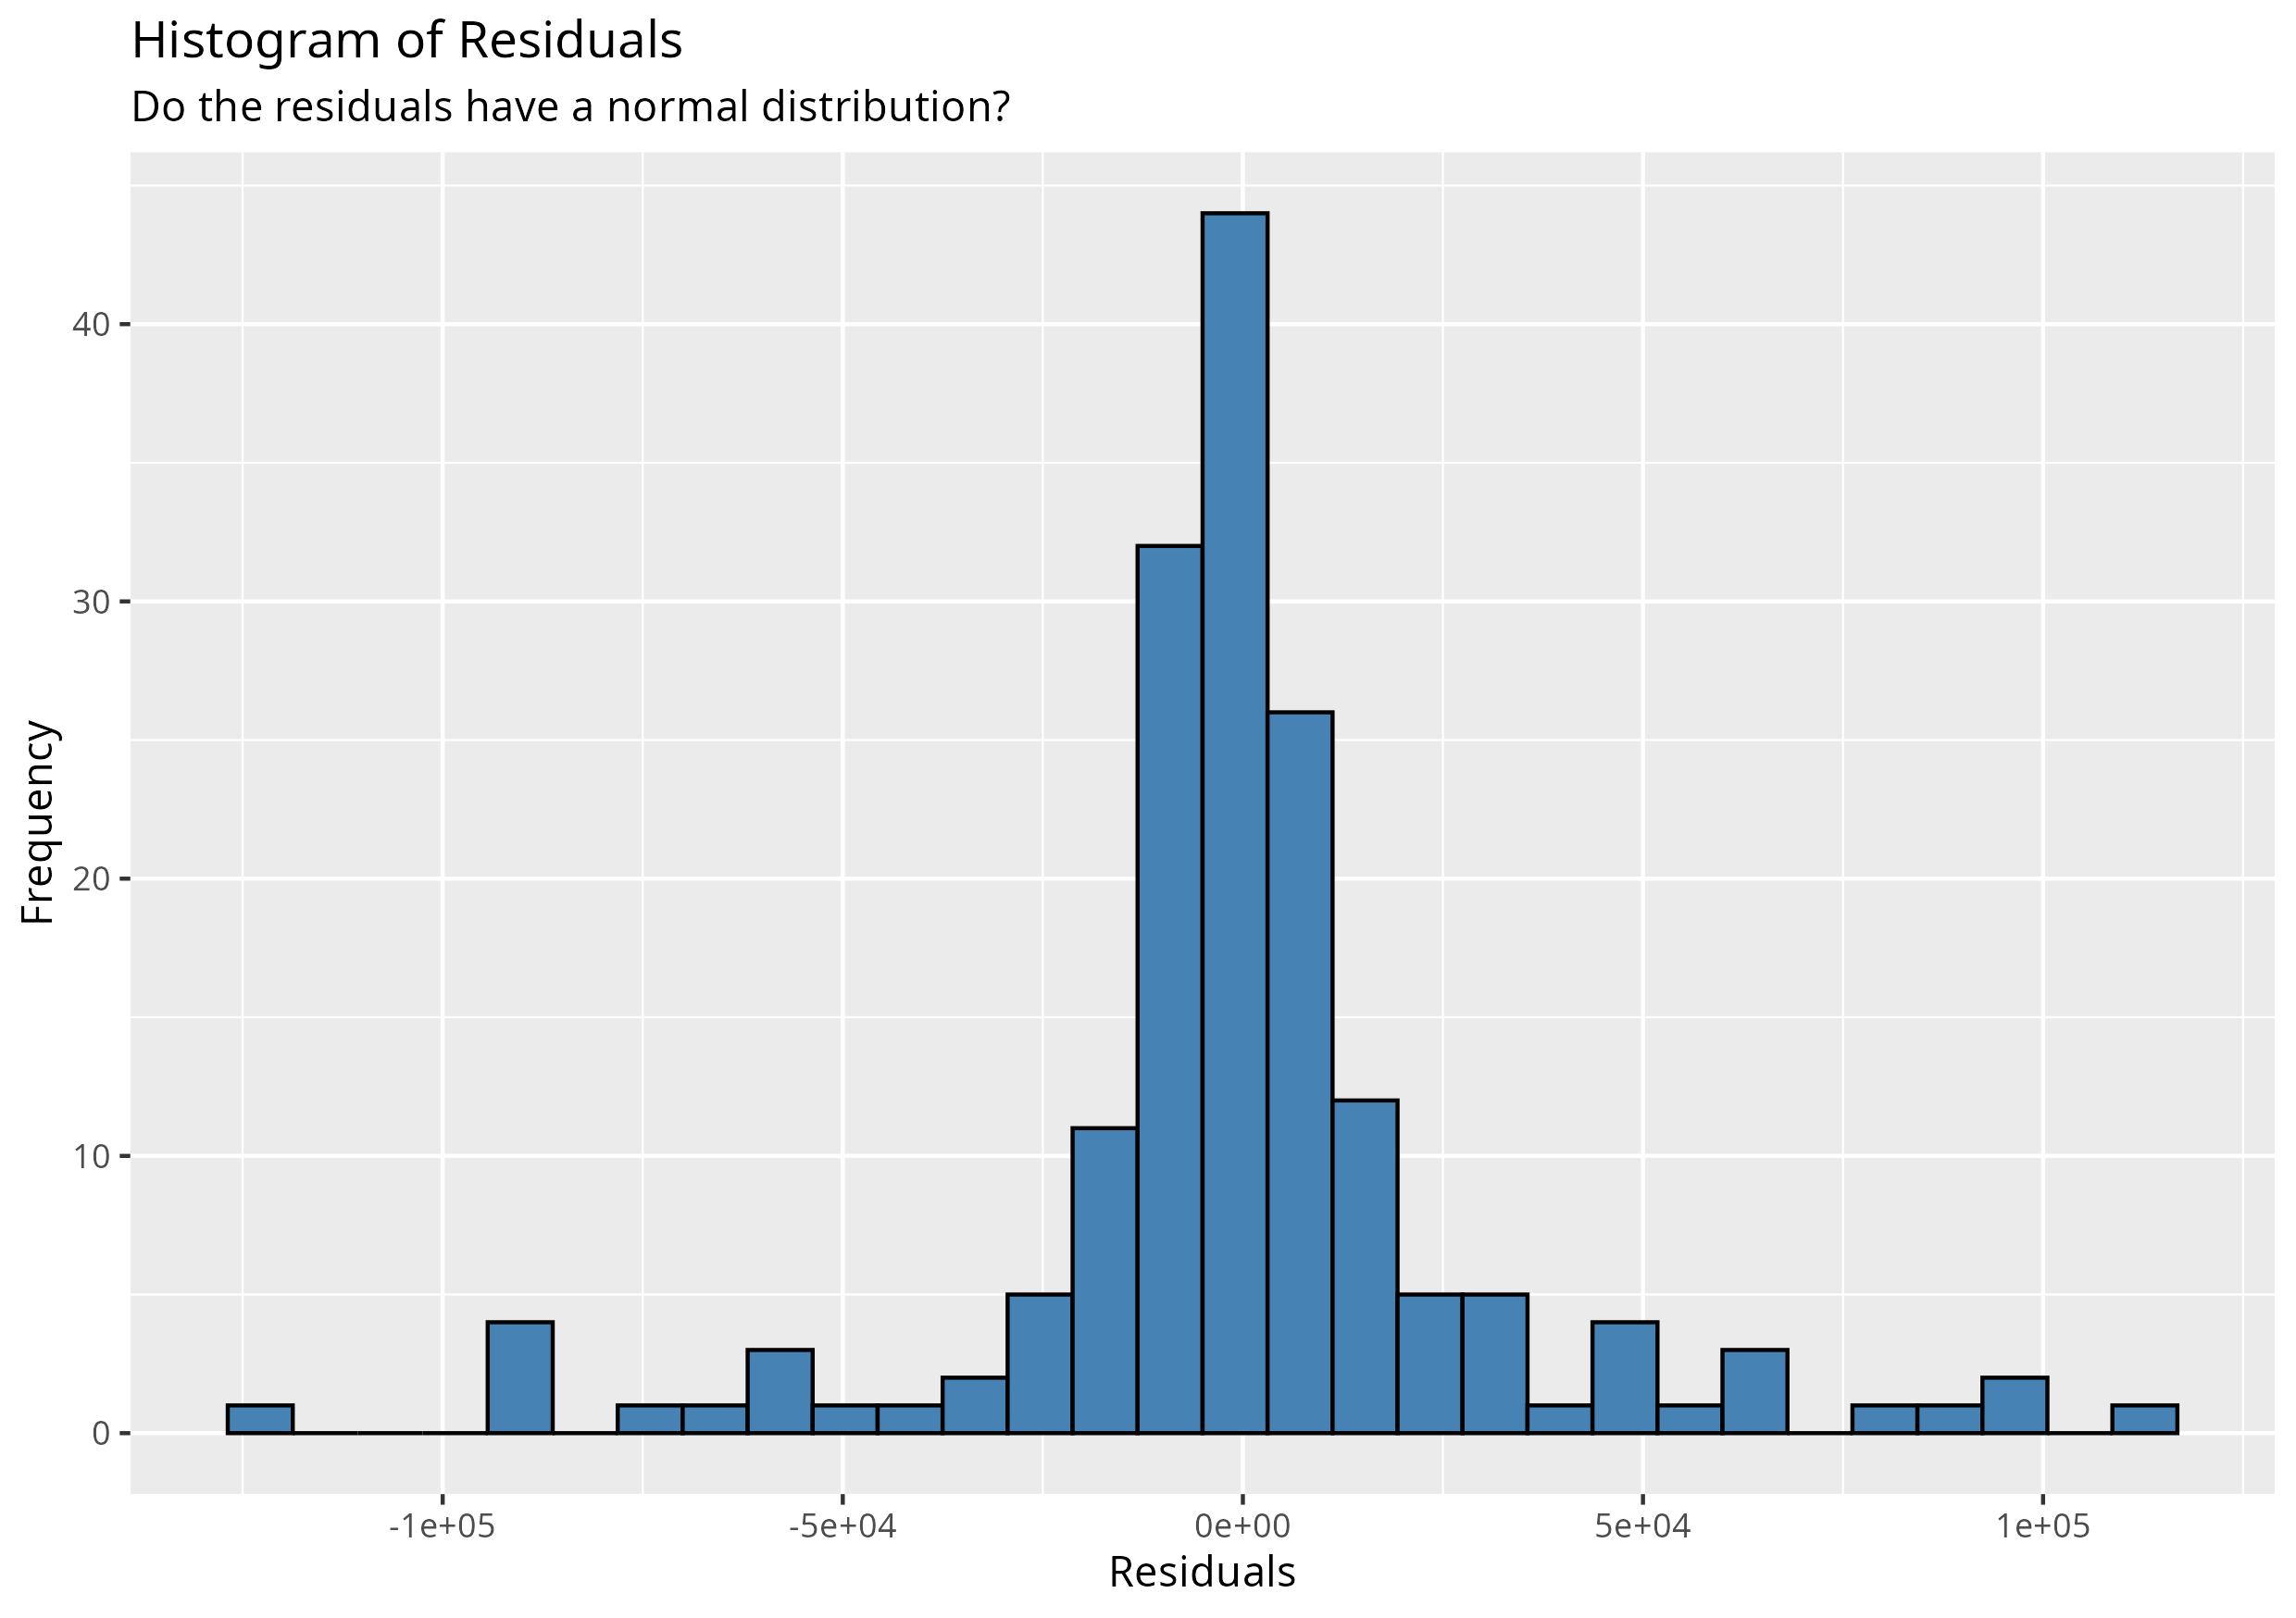
\includegraphics[scale=0.5]{figures/plot_residuals_hist_NPP-375-PM.png}
    \caption{Do the residuals have a normal distribution?}
  \end{figure}
\end{frame}

\subsubsection{AQUA M T}

\begin{frame}
  AQUA M T
\end{frame}

\begin{frame}
  \frametitle{Time series trend (with smoothing)}
  \begin{figure}
    \centering
    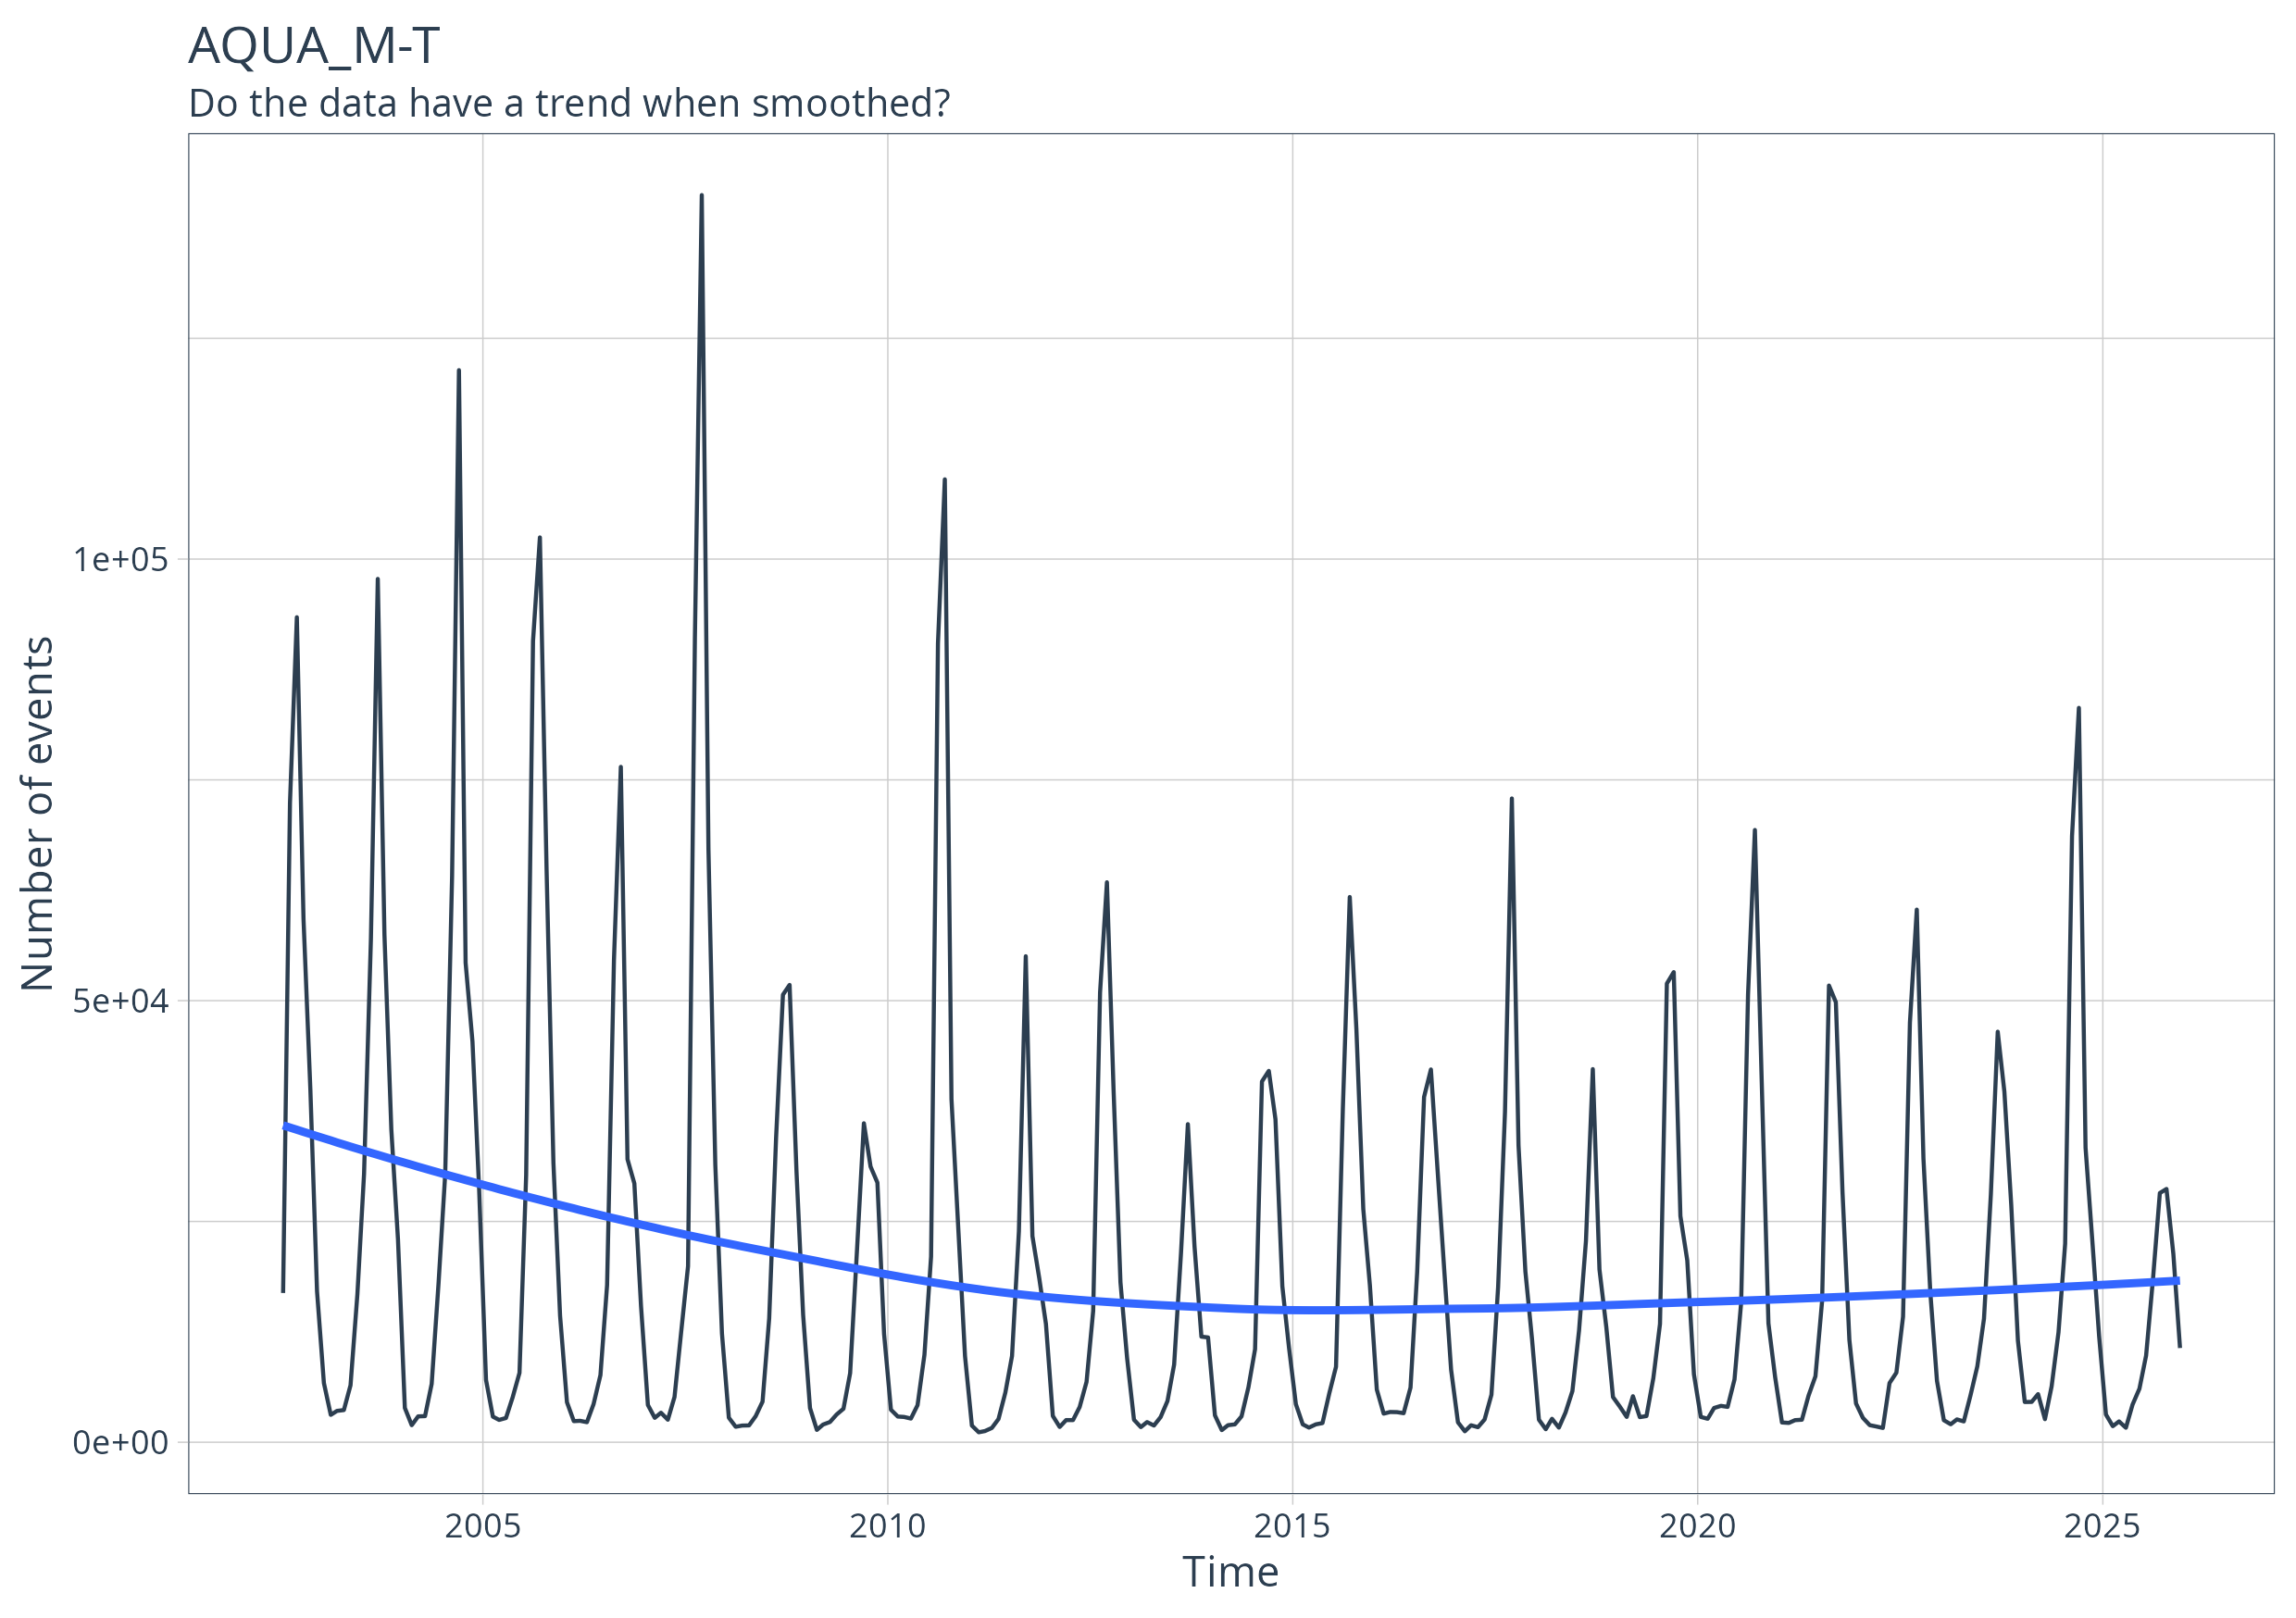
\includegraphics[scale=0.35]{figures/plot_trend_smoothing_AQUA_M-T.png}
    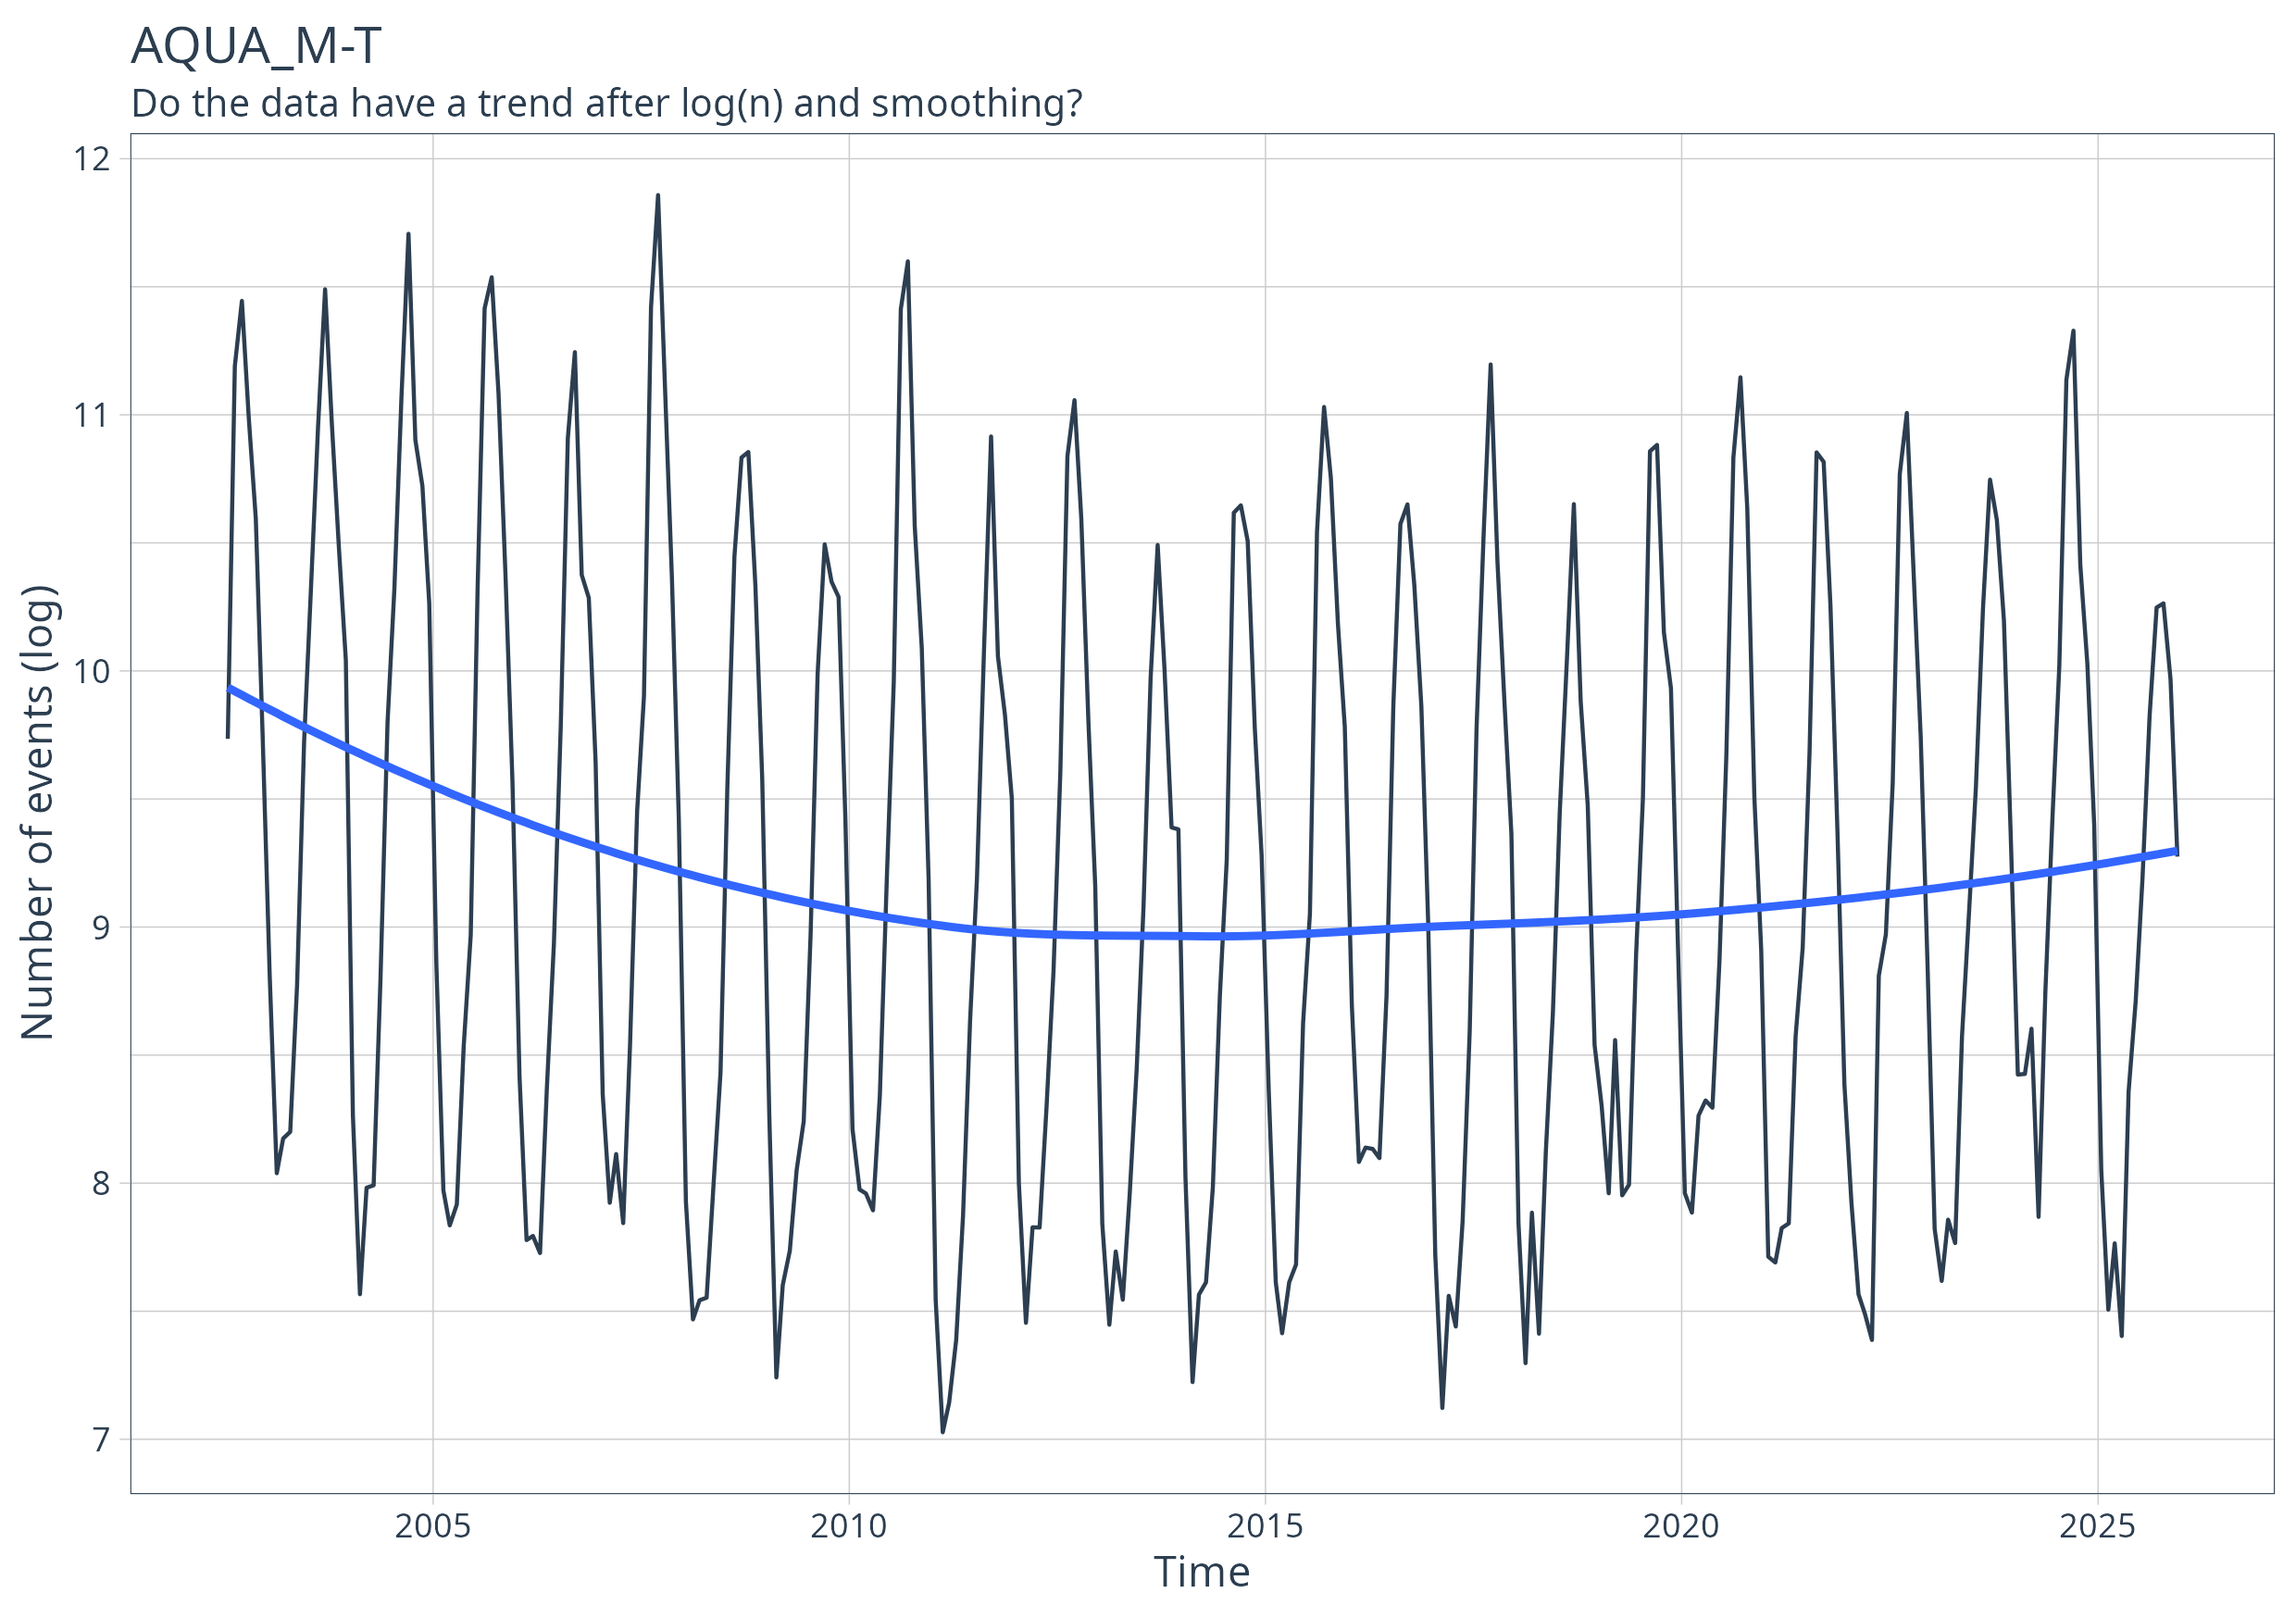
\includegraphics[scale=0.35]{figures/plot_trend_smoothing_log_AQUA_M-T.png}
    \caption{Do the data have trend when smoothed?}
  \end{figure}
\end{frame}

\begin{frame}
  \frametitle{Time series autocorrelation}
  \begin{figure}
    \centering
    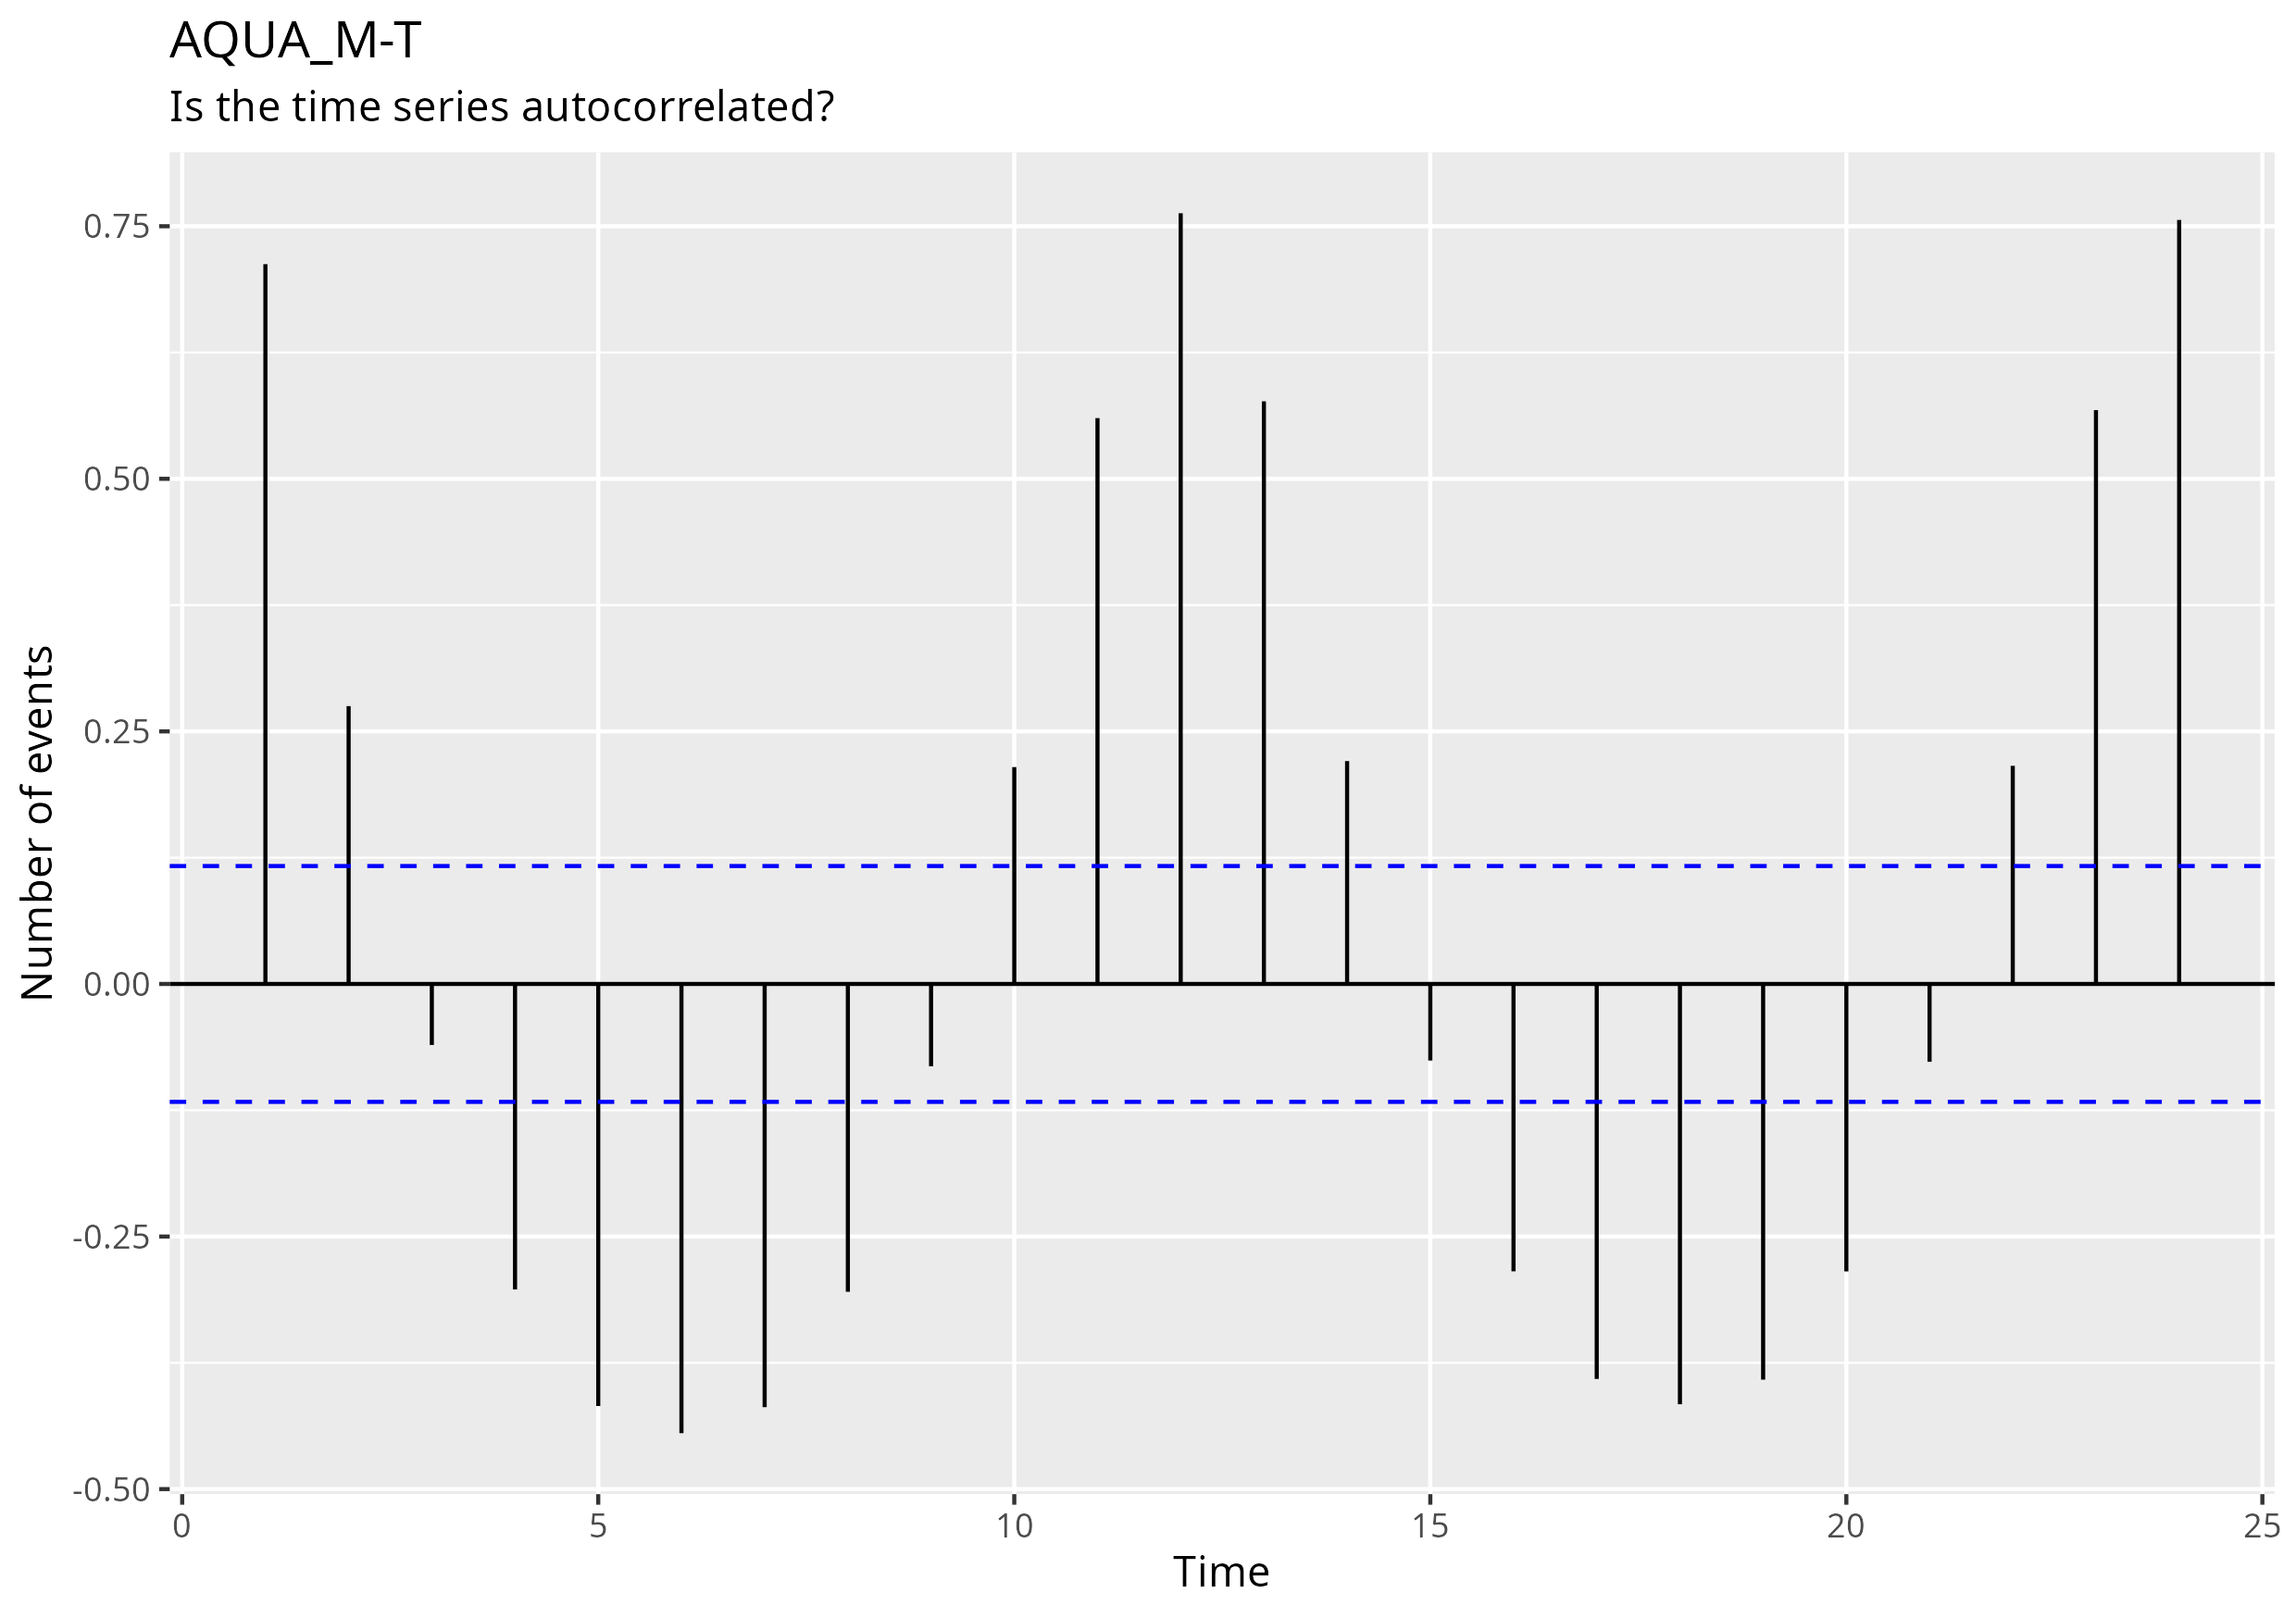
\includegraphics[scale=0.45]{figures/plot_autocorrelation_AQUA_M-T.png}
    \caption{Is the time series autocorrelated?}
  \end{figure}
\end{frame}

\begin{frame}
  \frametitle{Time series trend}
  \begin{figure}
    \centering
    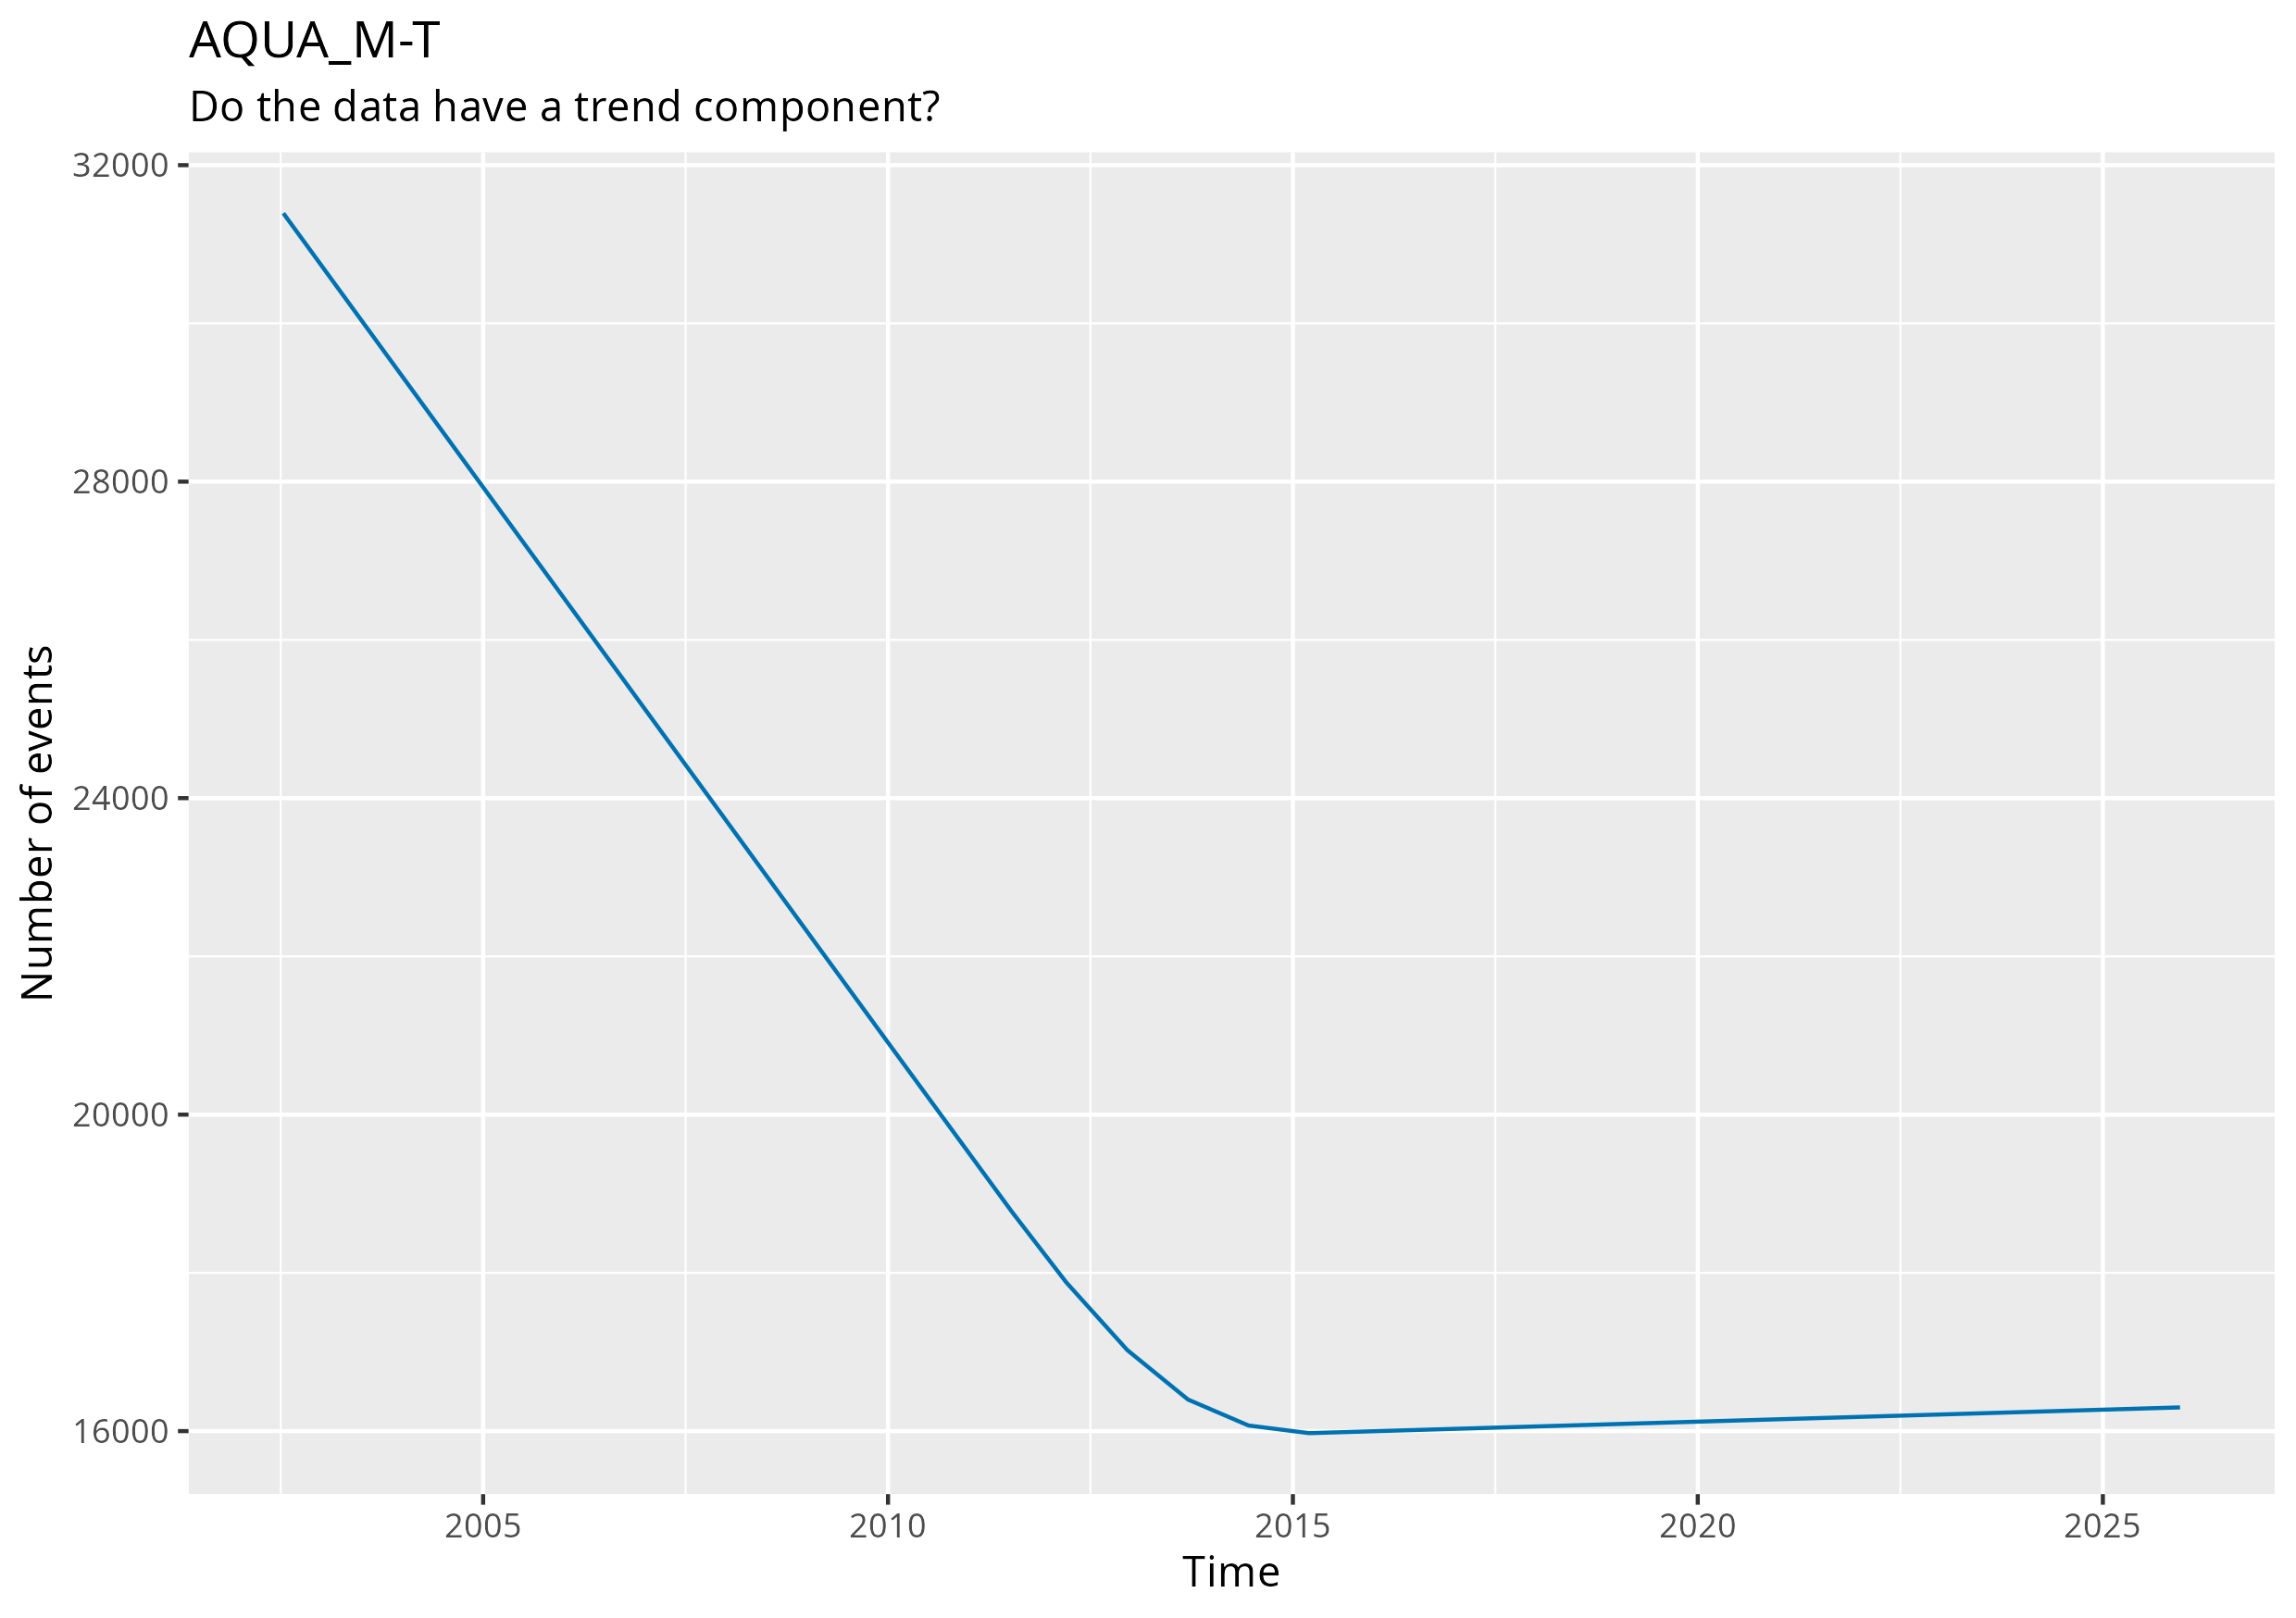
\includegraphics[scale=0.45]{figures/plot_component_trend_AQUA_M-T.png}
    \caption{Do the data have a trend component?}
  \end{figure}
\end{frame}

\begin{frame}
  \frametitle{Time series seasonality}
  \begin{figure}
    \centering
    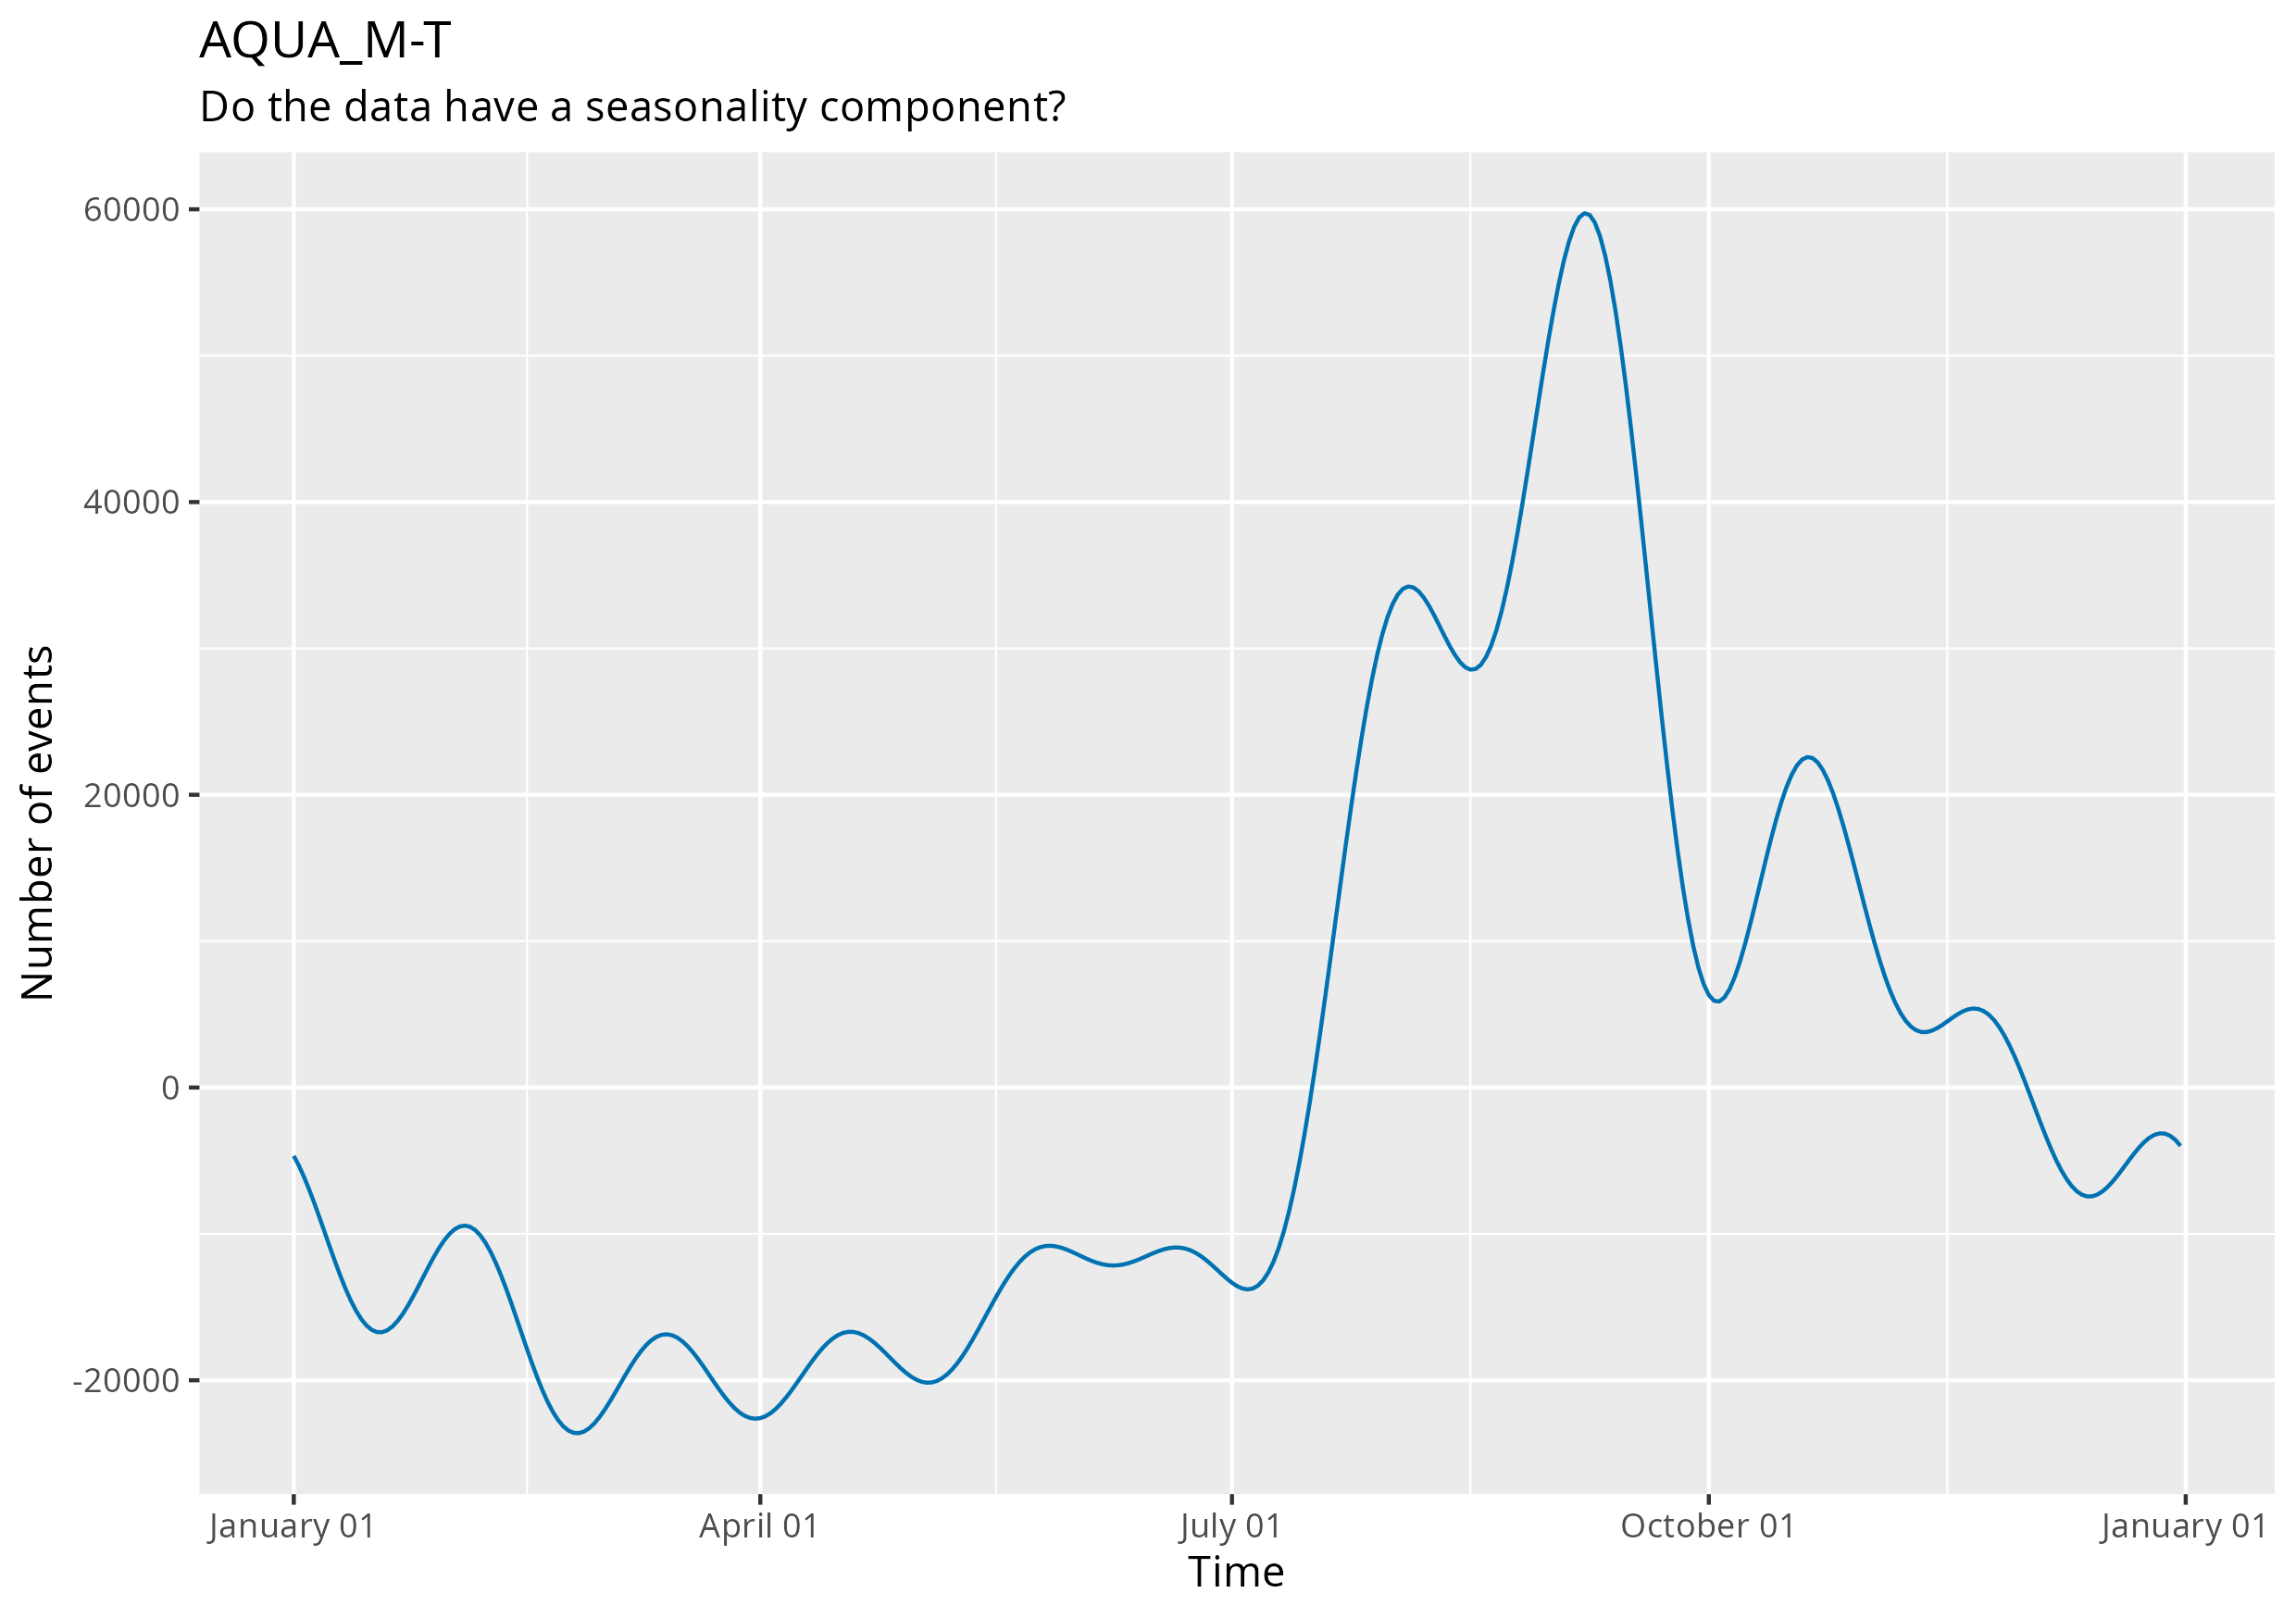
\includegraphics[scale=0.45]{figures/plot_component_seasonality_AQUA_M-T.png}
    \caption{Do the data have a seasonality component?}
  \end{figure}
\end{frame}

\begin{frame}
  \frametitle{Time series versus forecast}
  \begin{figure}
    \centering
    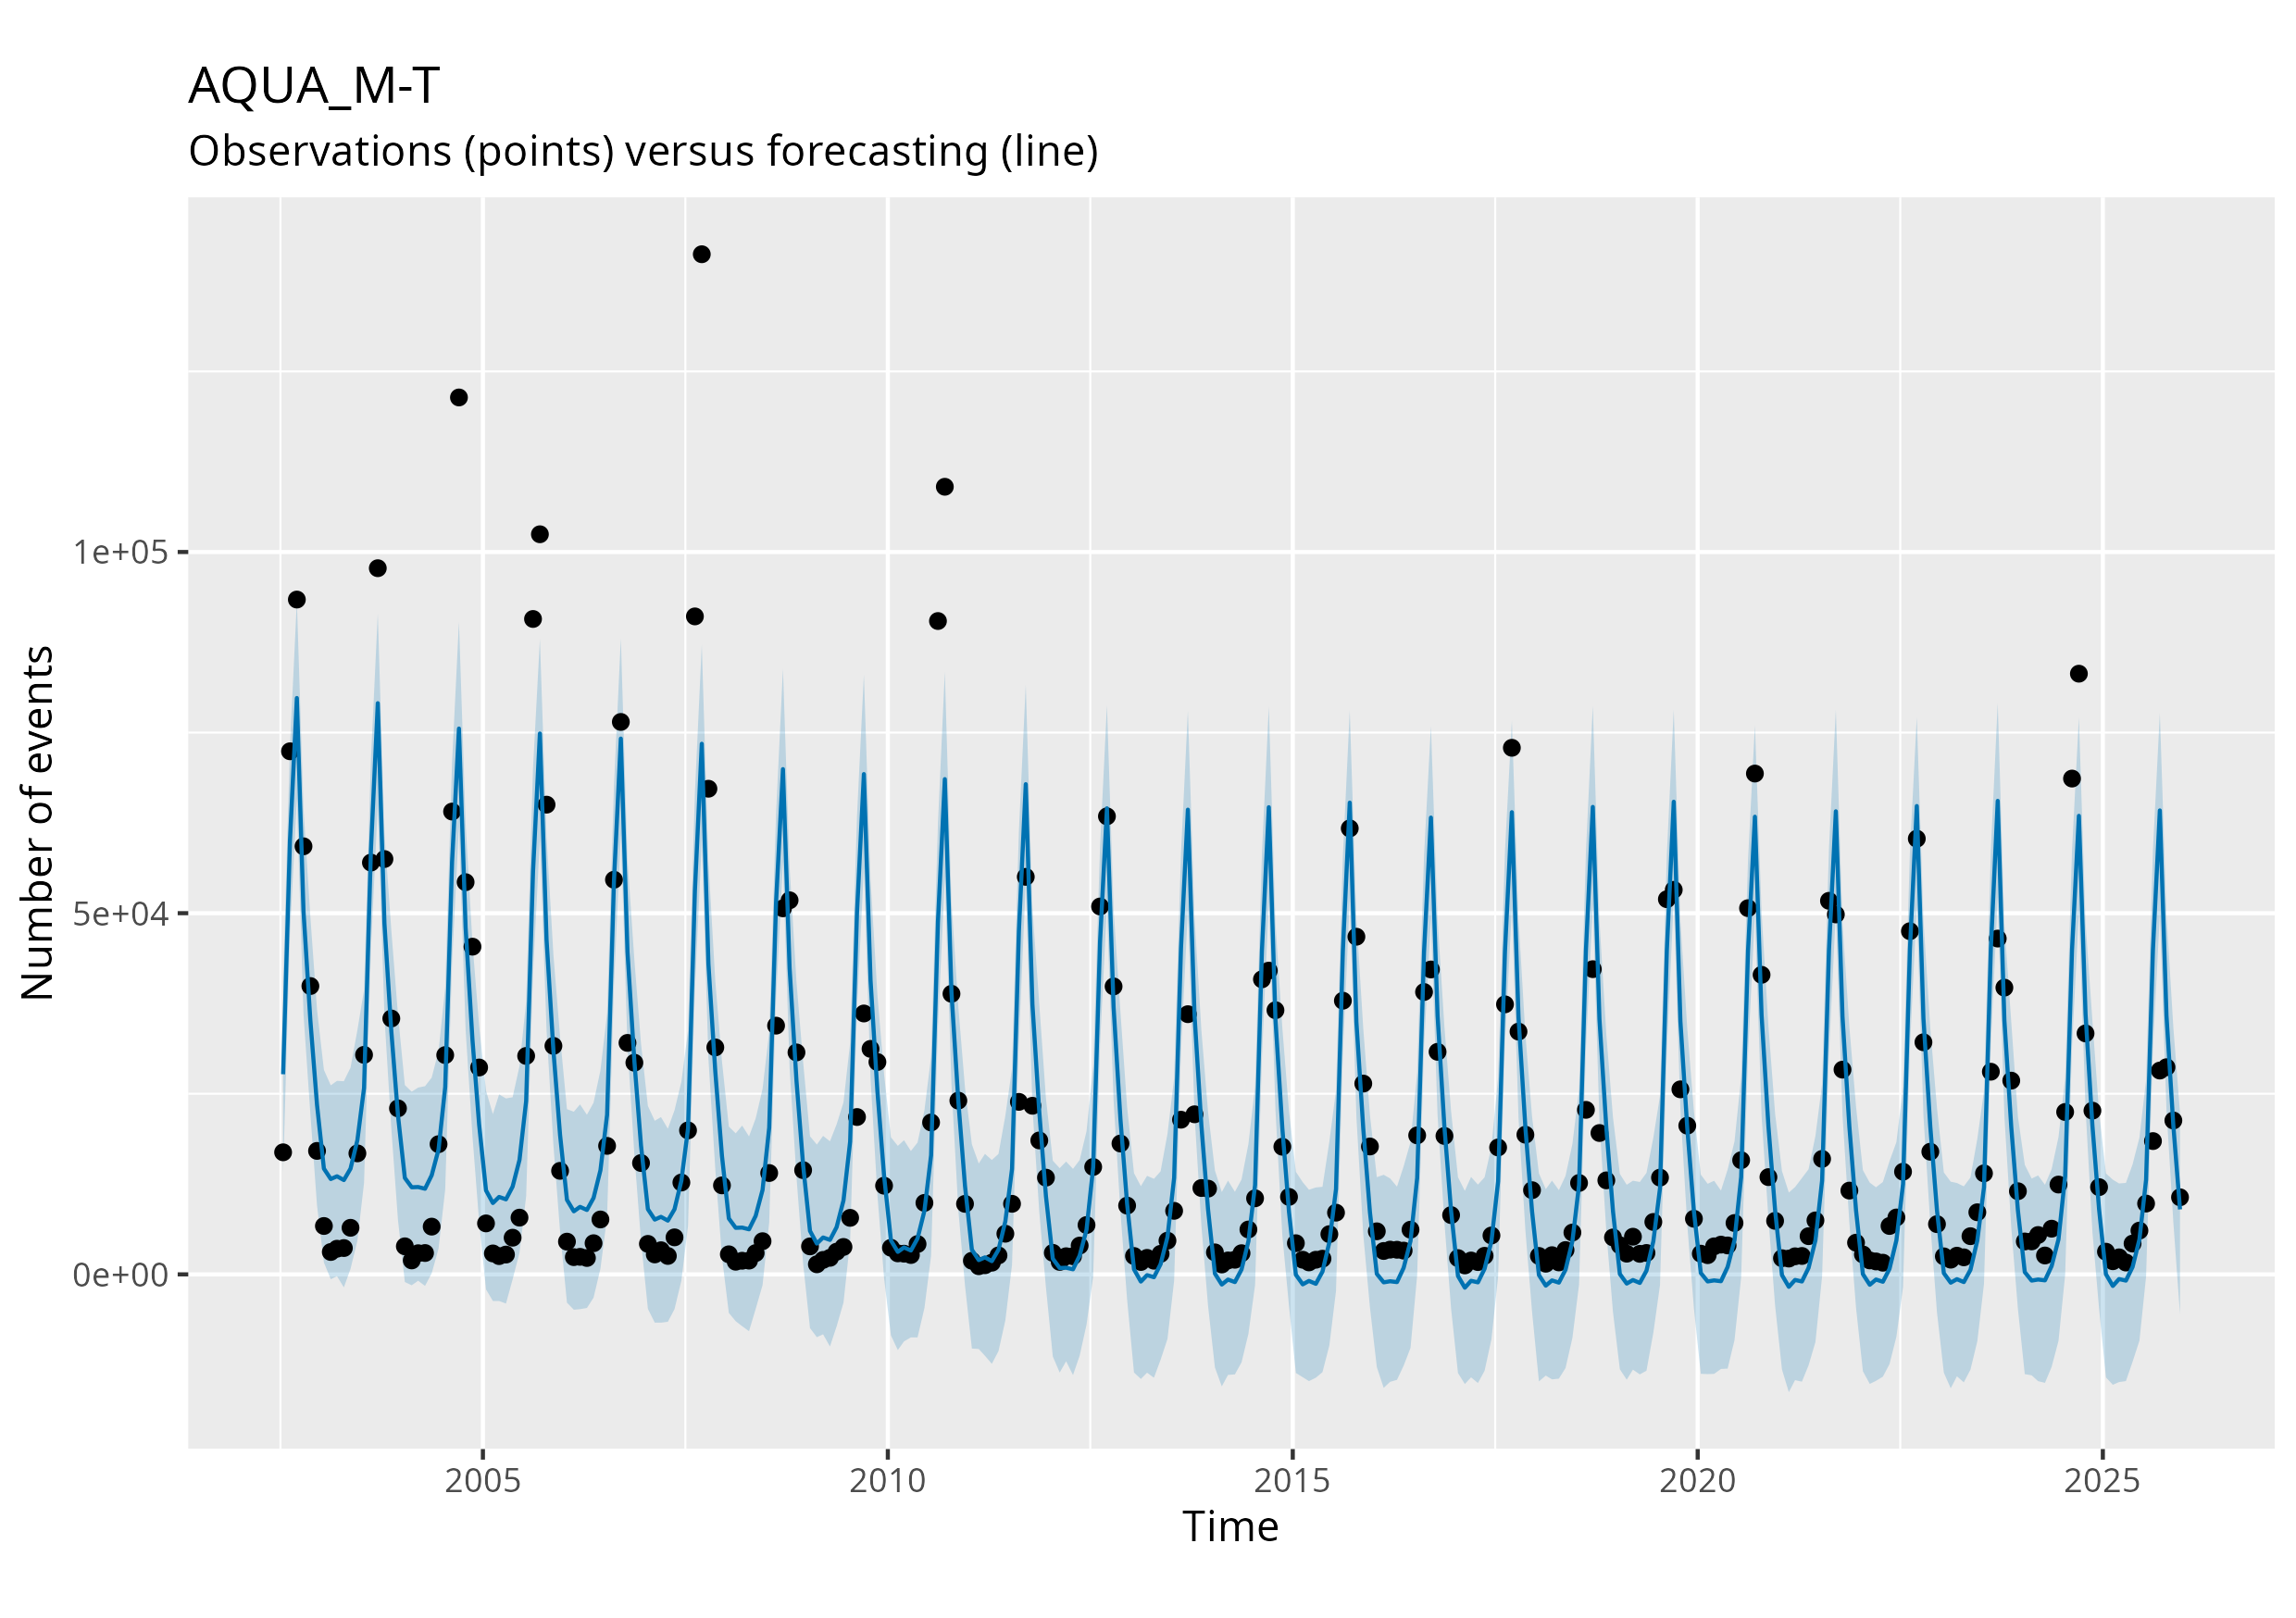
\includegraphics[scale=0.45]{figures/plot_model_forecast_AQUA_M-T.png}
    \caption{Observations (black dots), model (blue line), and 95\% confidence
    interval (gray shadow).}
  \end{figure}
\end{frame}

\begin{frame}
  \frametitle{Time series versus forecast}
  \begin{figure}
    \centering
    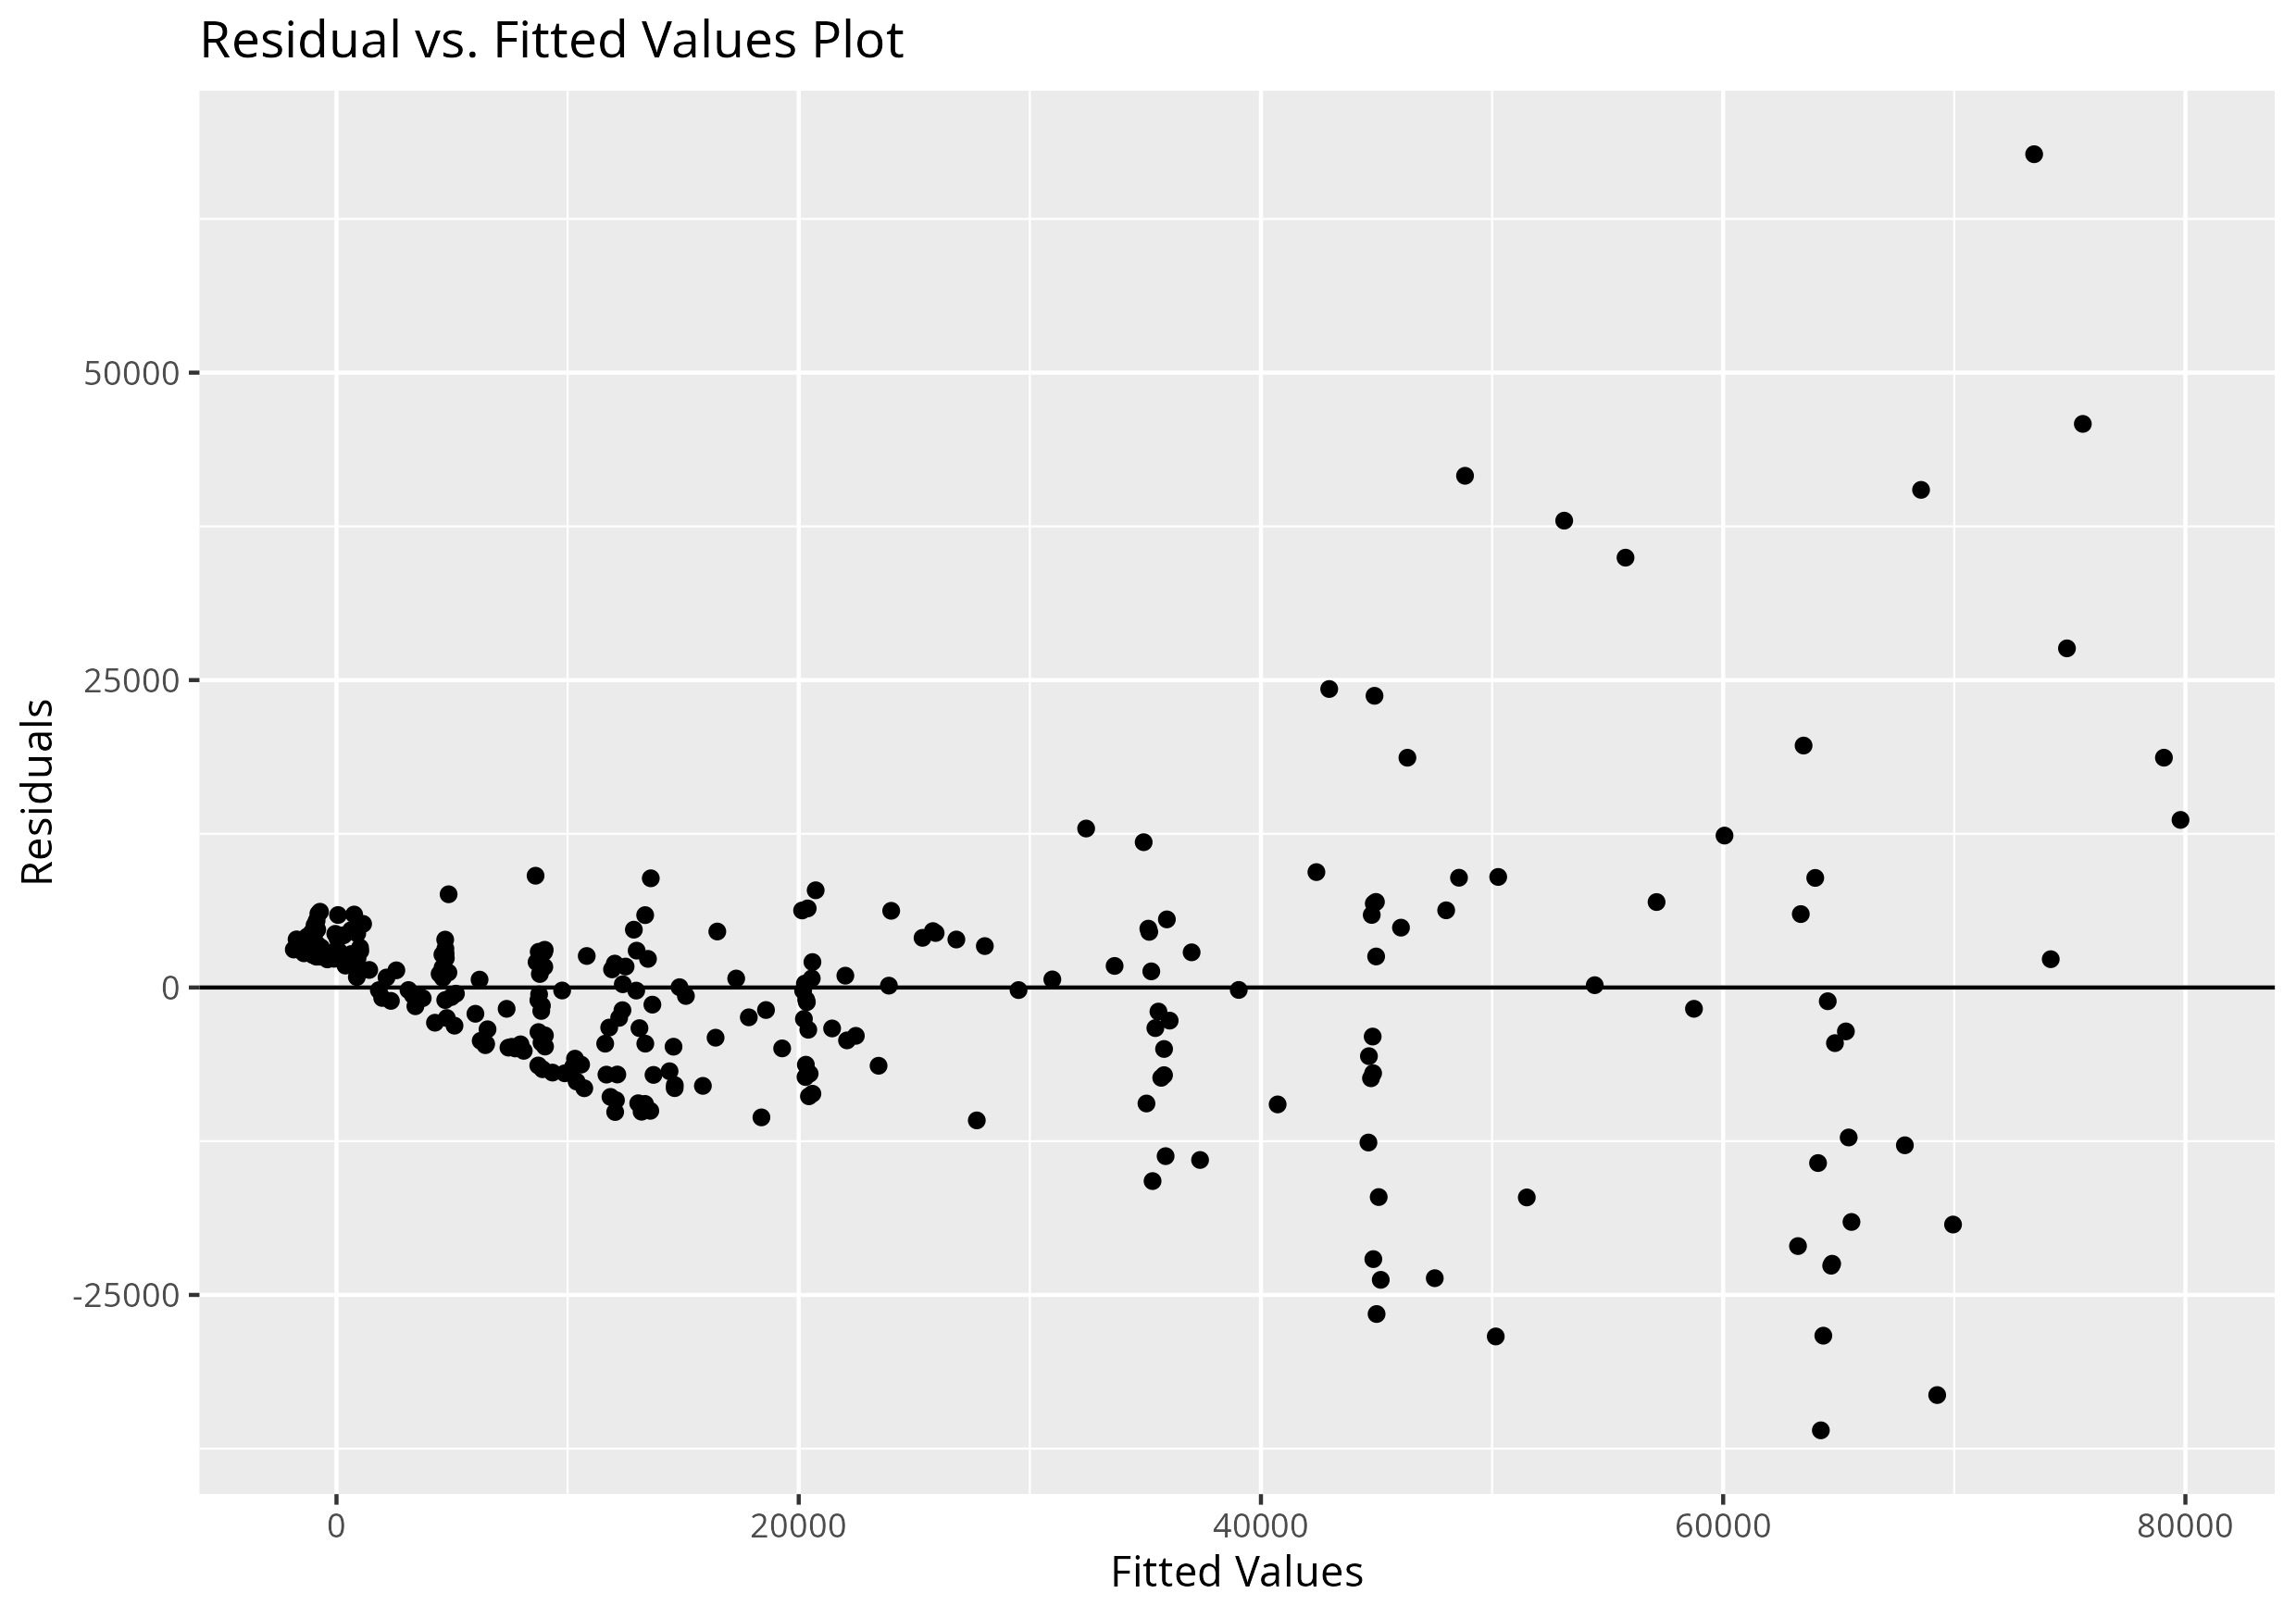
\includegraphics[scale=0.5]{figures/plot_residuals_AQUA_M-T.png}
    \caption{Larger fitted fire foci values have larger residuals.}
  \end{figure}
\end{frame}

\begin{frame}
  \frametitle{Time series versus forecast}
  \begin{figure}
    \centering
    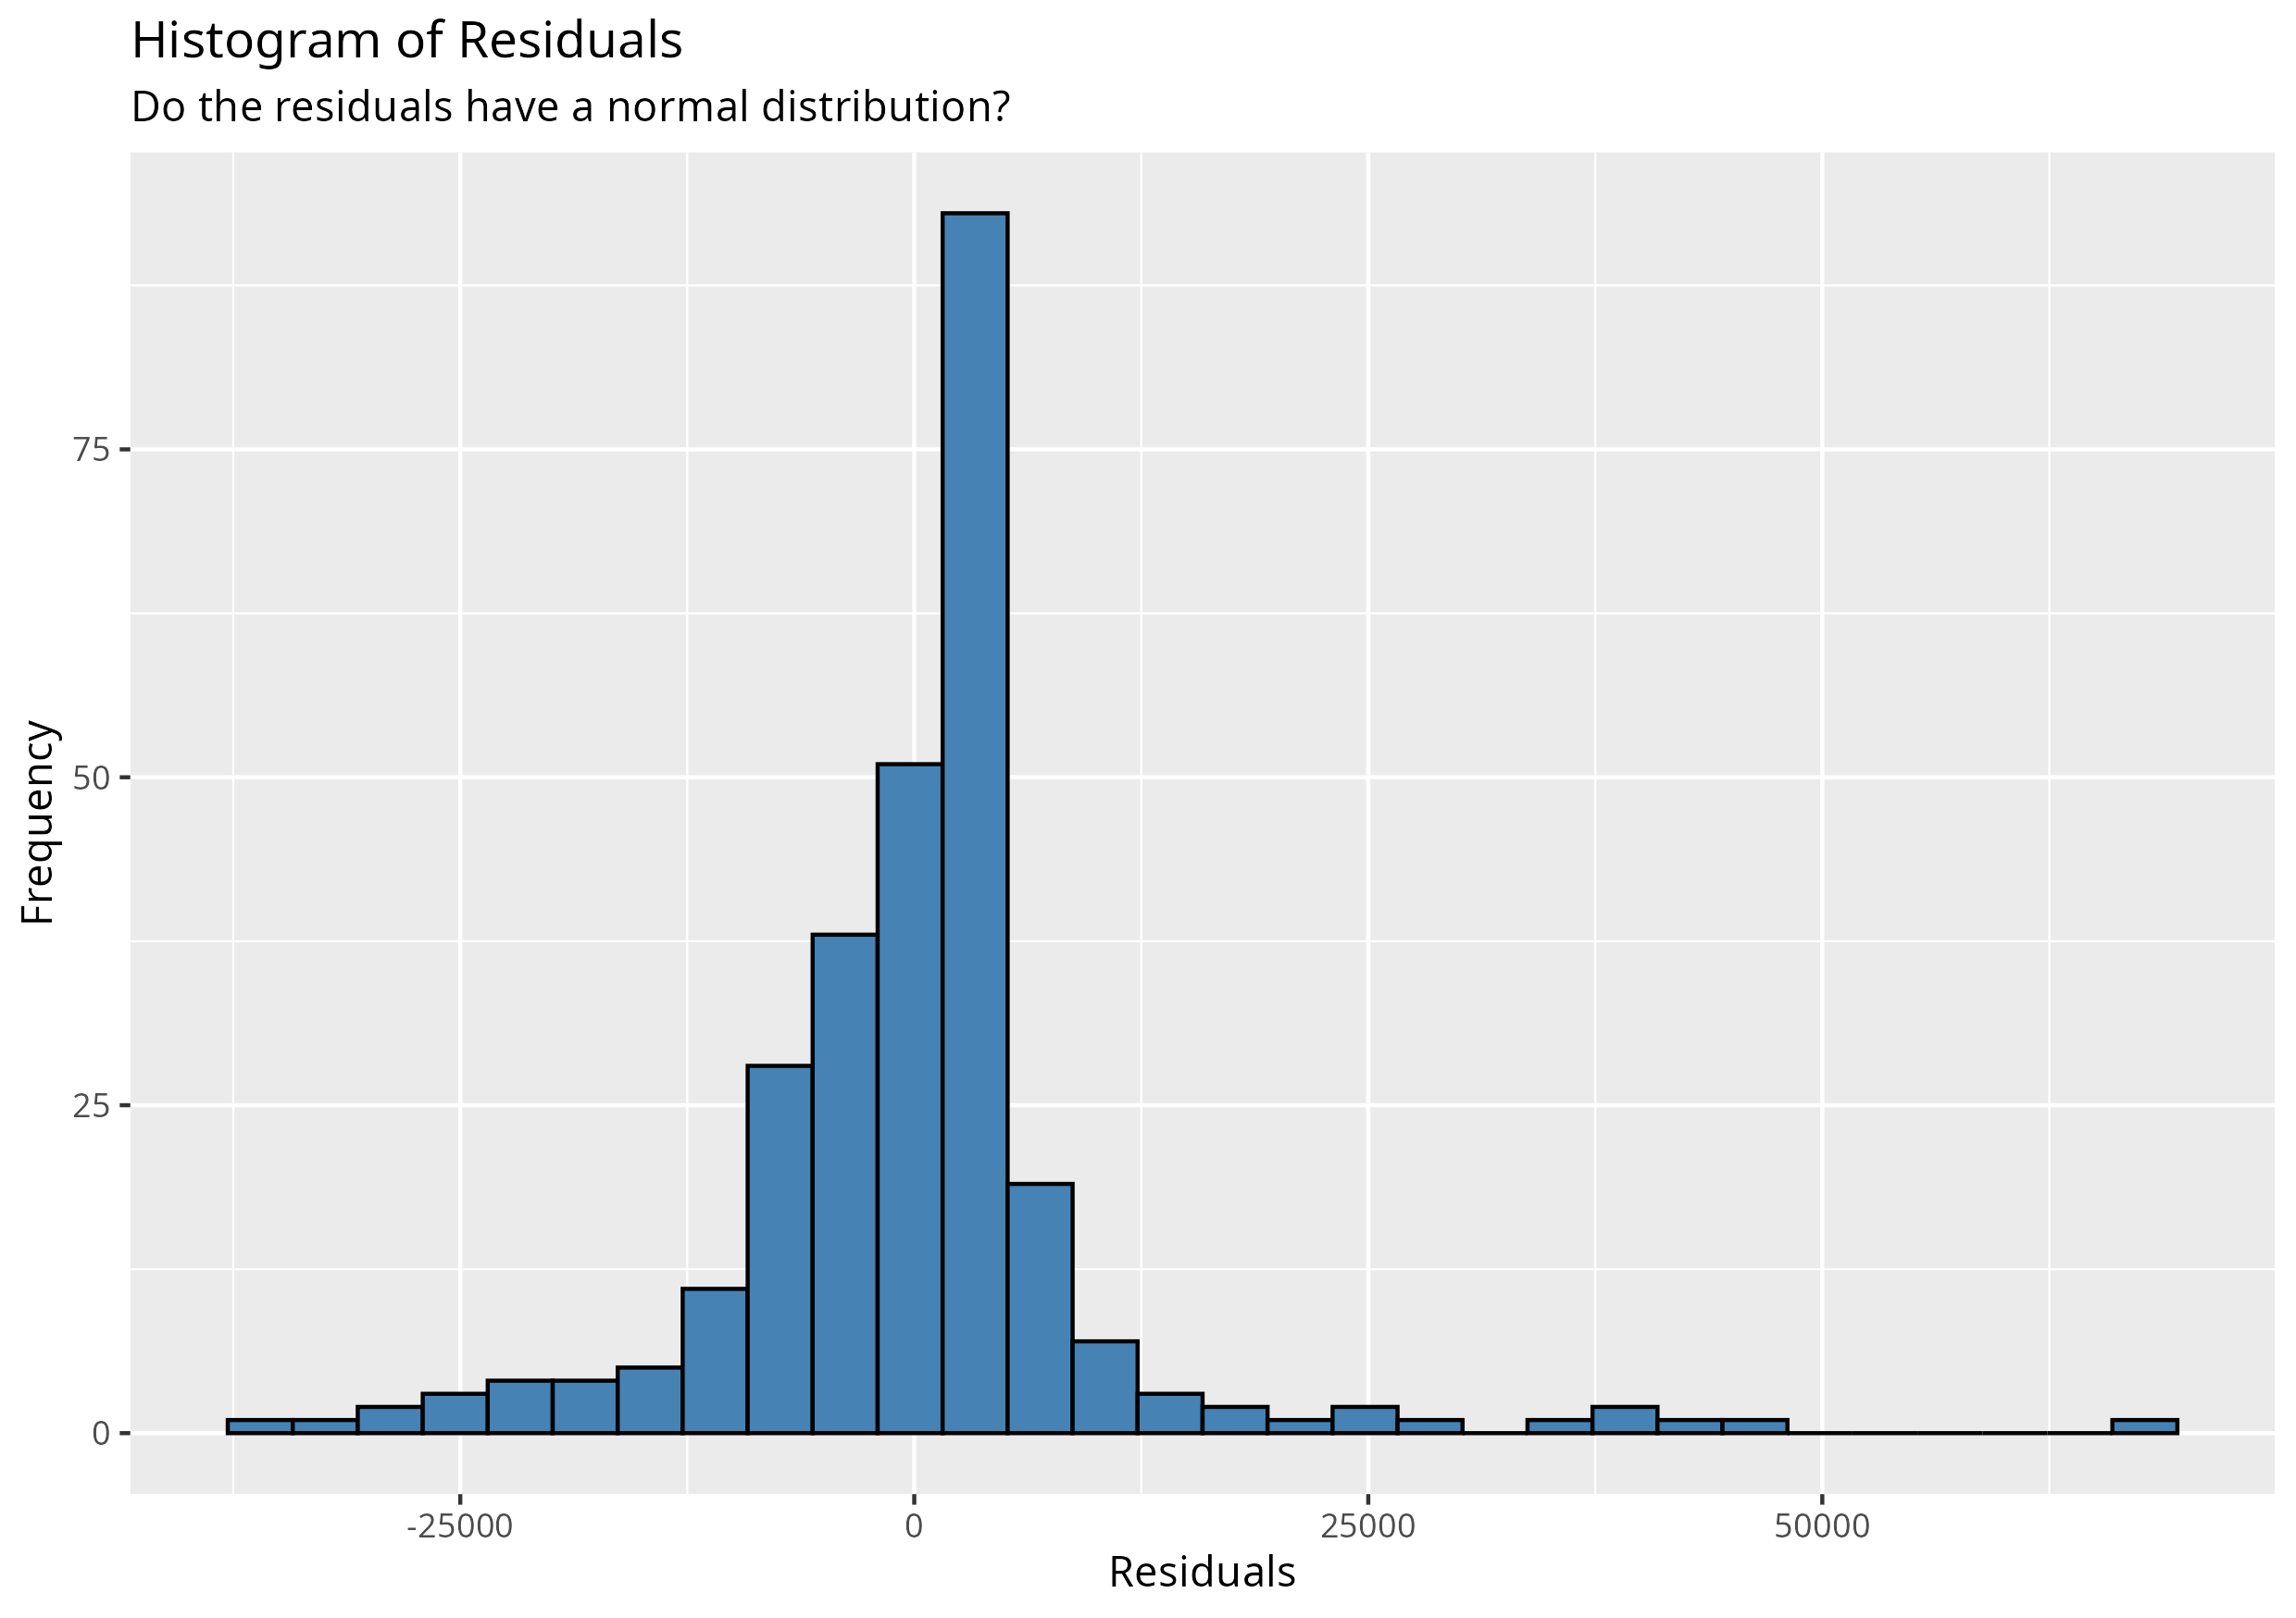
\includegraphics[scale=0.5]{figures/plot_residuals_hist_AQUA_M-T.png}
    \caption{Do the residuals have a normal distribution?}
  \end{figure}
\end{frame}

\subsubsection{NOAA 12}

\begin{frame}
  NOAA 12
\end{frame}

\begin{frame}
  \frametitle{Time series trend (with smoothing)}
  \begin{figure}
    \centering
    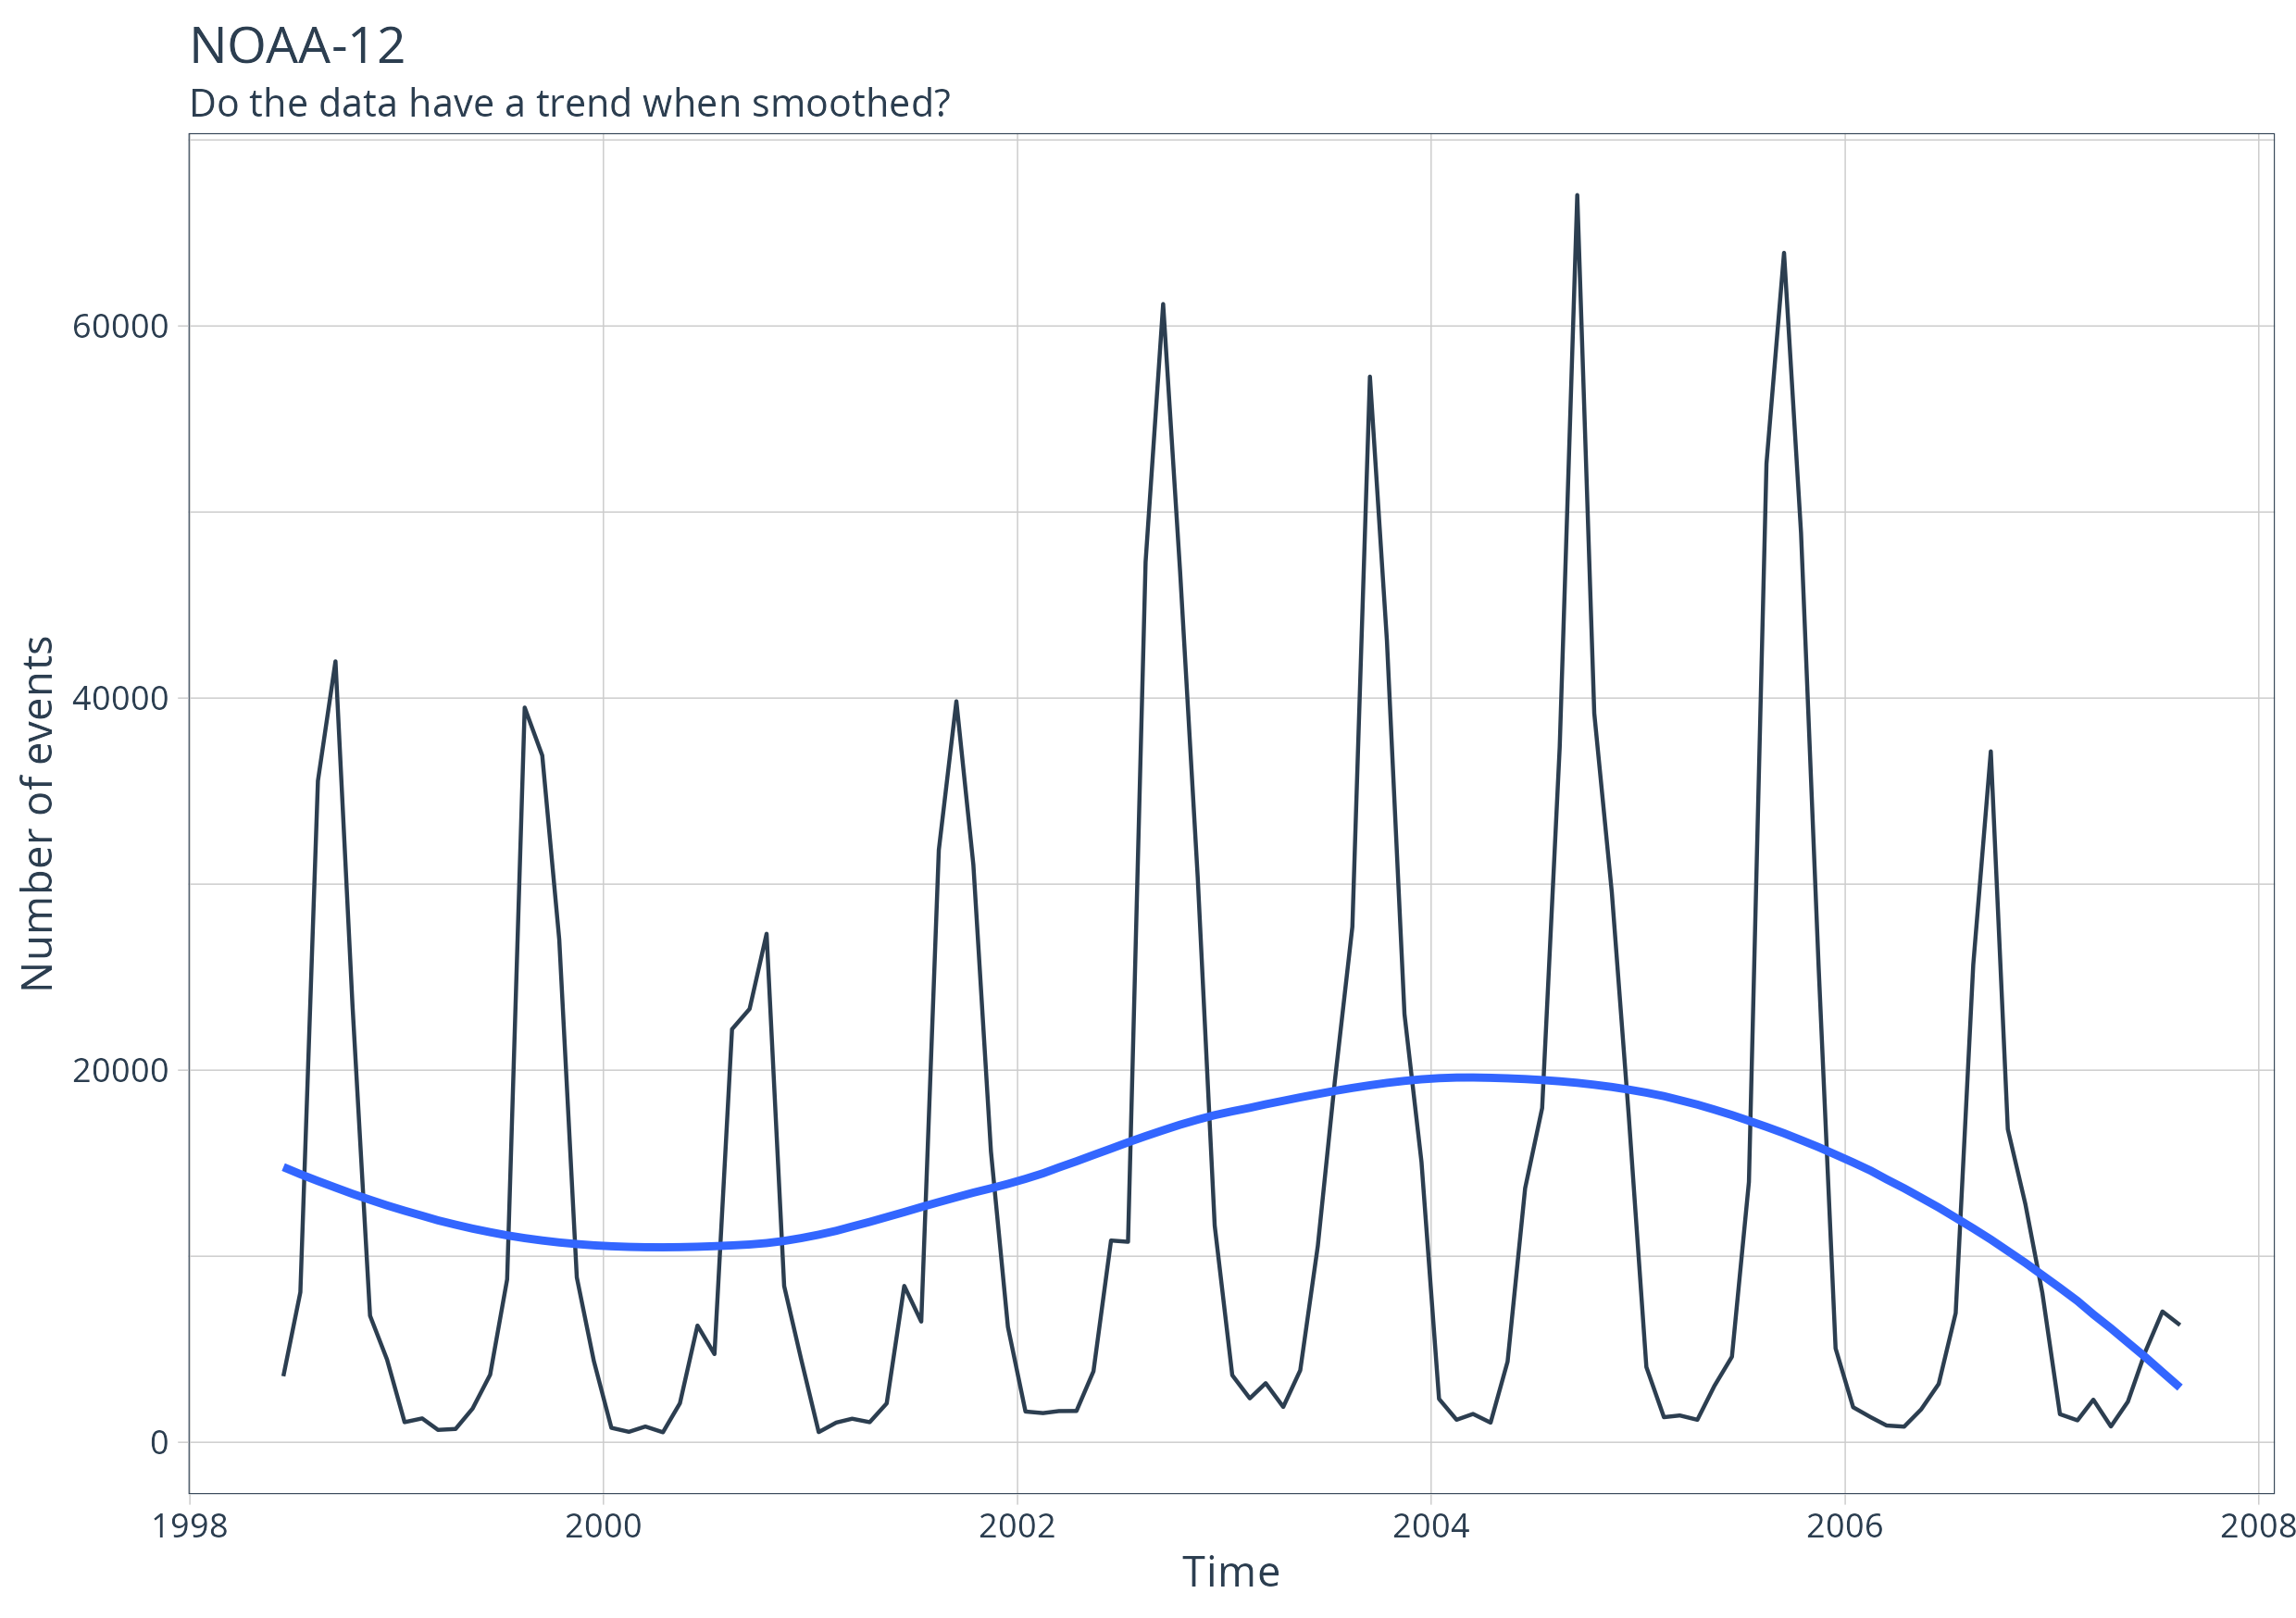
\includegraphics[scale=0.35]{figures/plot_trend_smoothing_NOAA-12.png}
    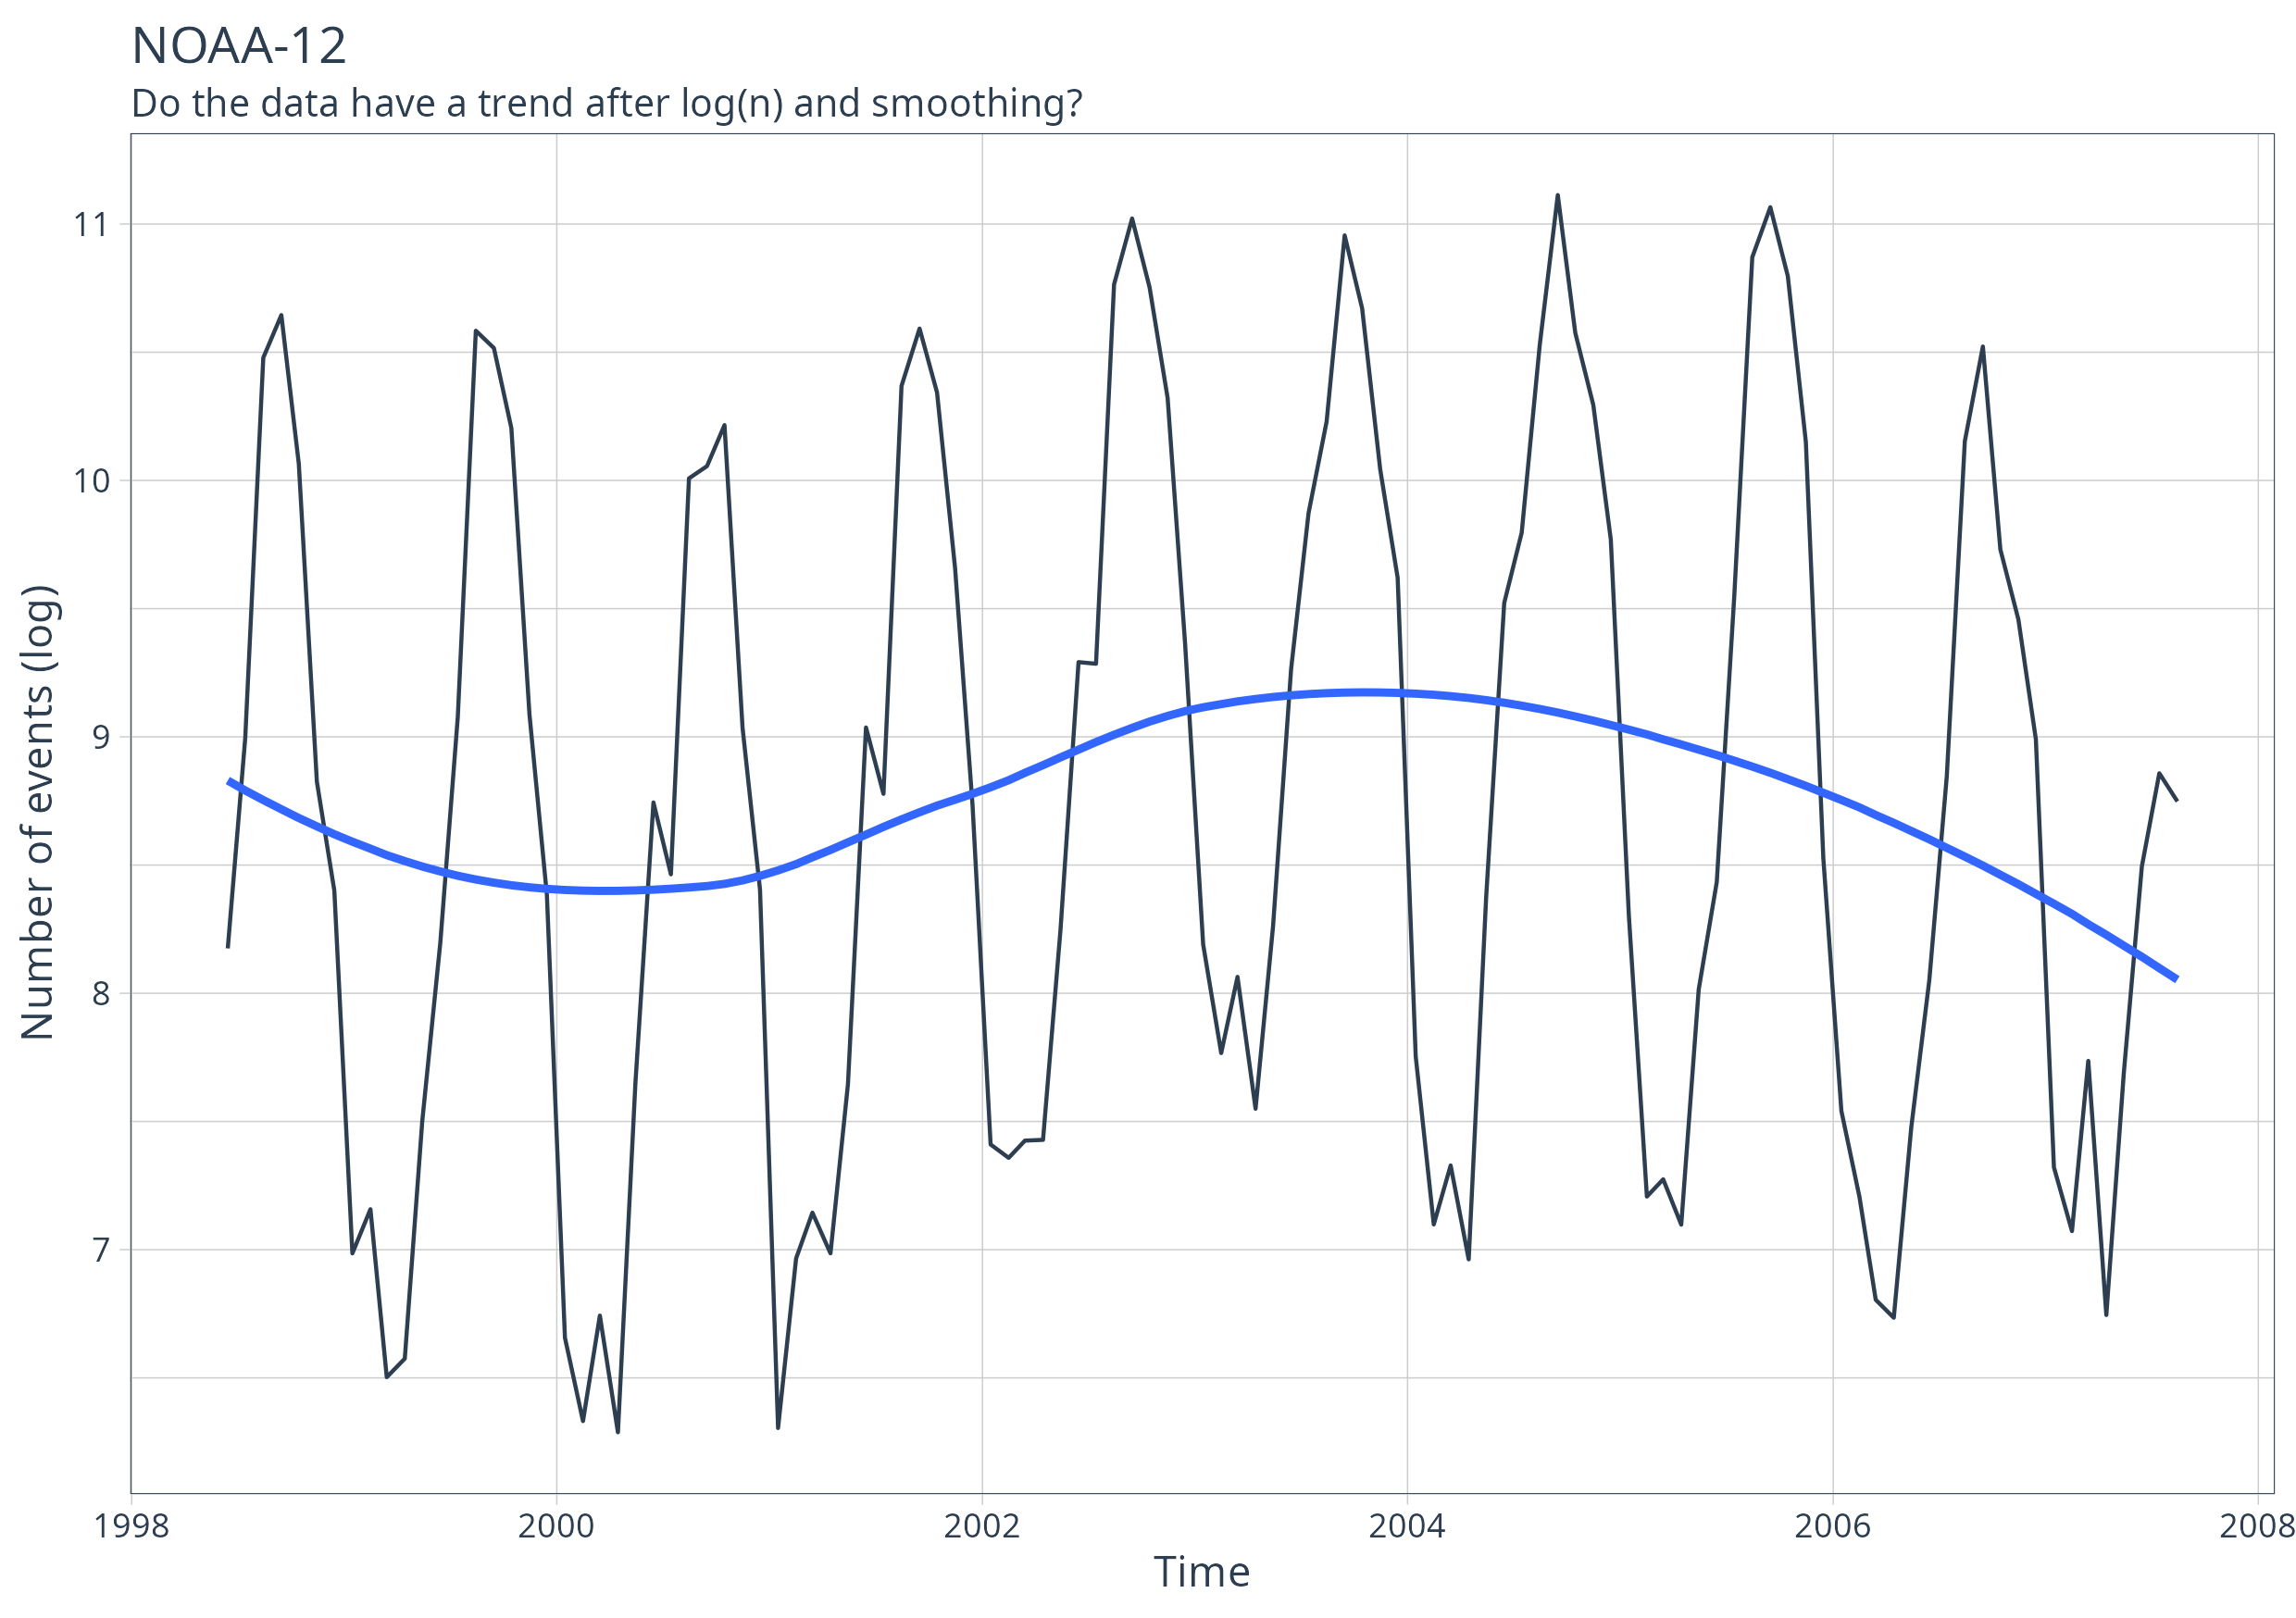
\includegraphics[scale=0.35]{figures/plot_trend_smoothing_log_NOAA-12.png}
    \caption{Do the data have a trend when smoothed?}
  \end{figure}
\end{frame}

\begin{frame}
  \frametitle{Time series autocorrelation}
  \begin{figure}
    \centering
    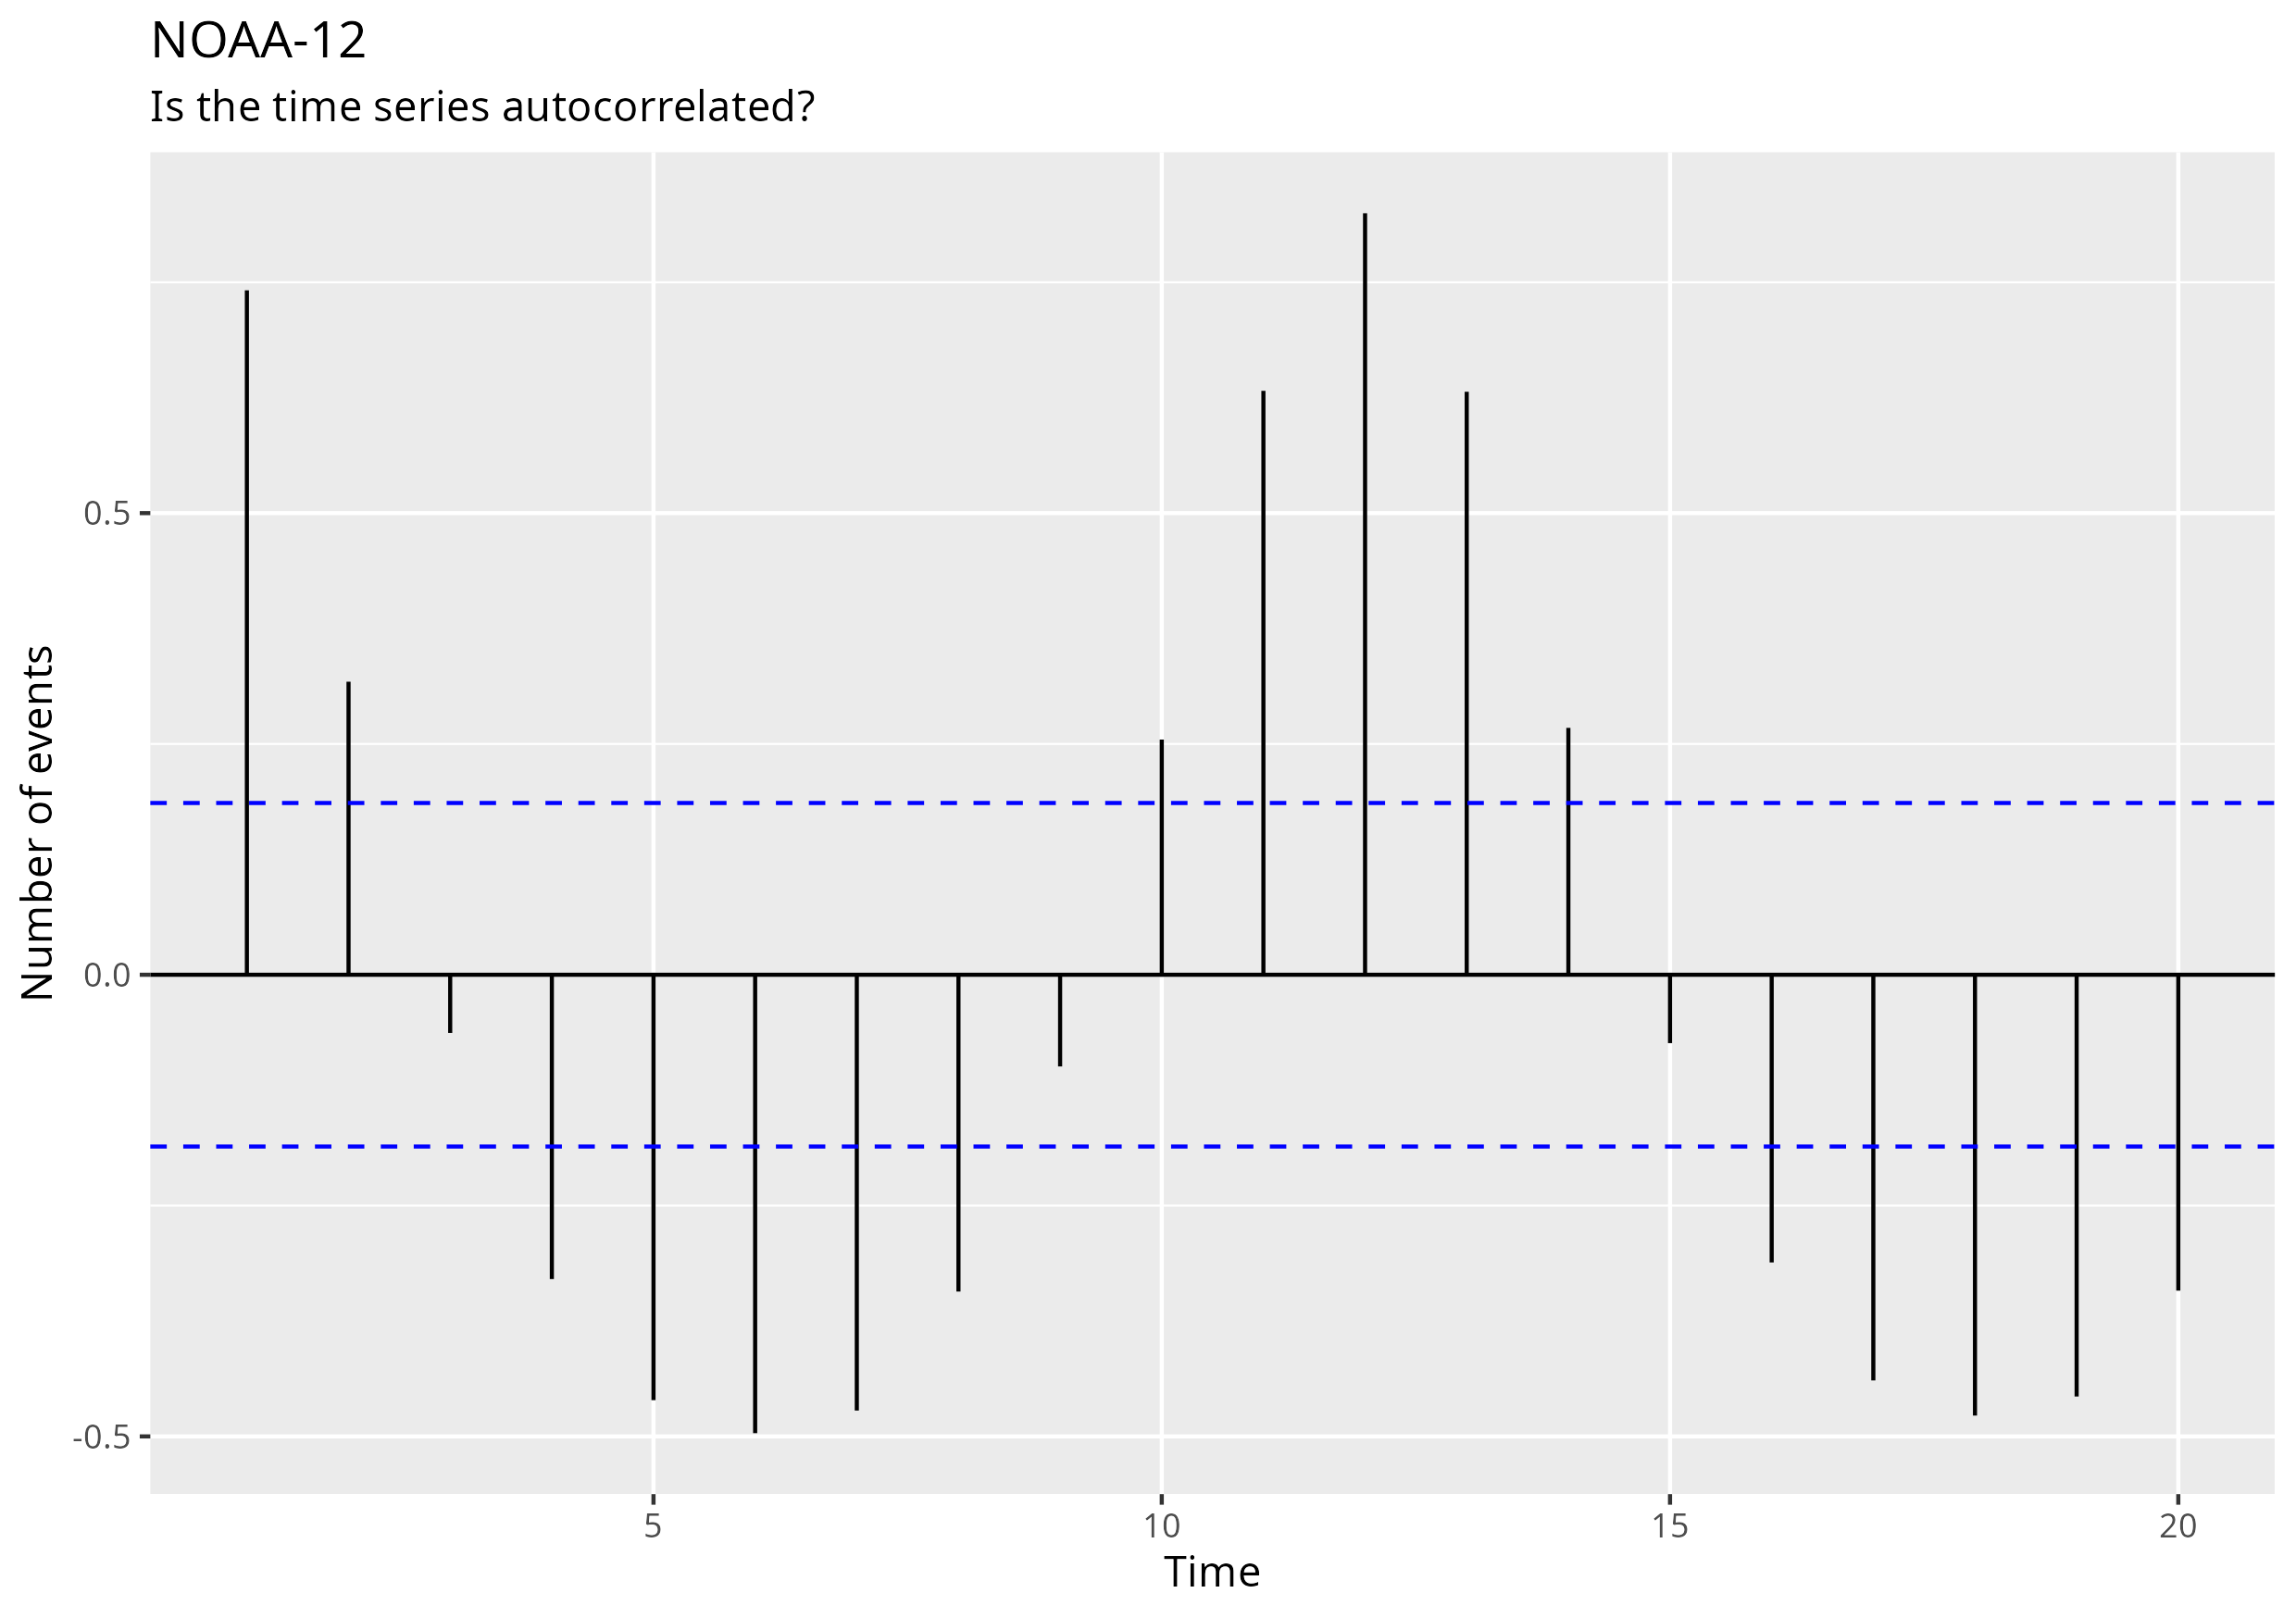
\includegraphics[scale=0.45]{figures/plot_autocorrelation_NOAA-12.png}
    \caption{Is the time series autocorrelated?}
  \end{figure}
\end{frame}

\begin{frame}
  \frametitle{Time series trend}
  \begin{figure}
    \centering
    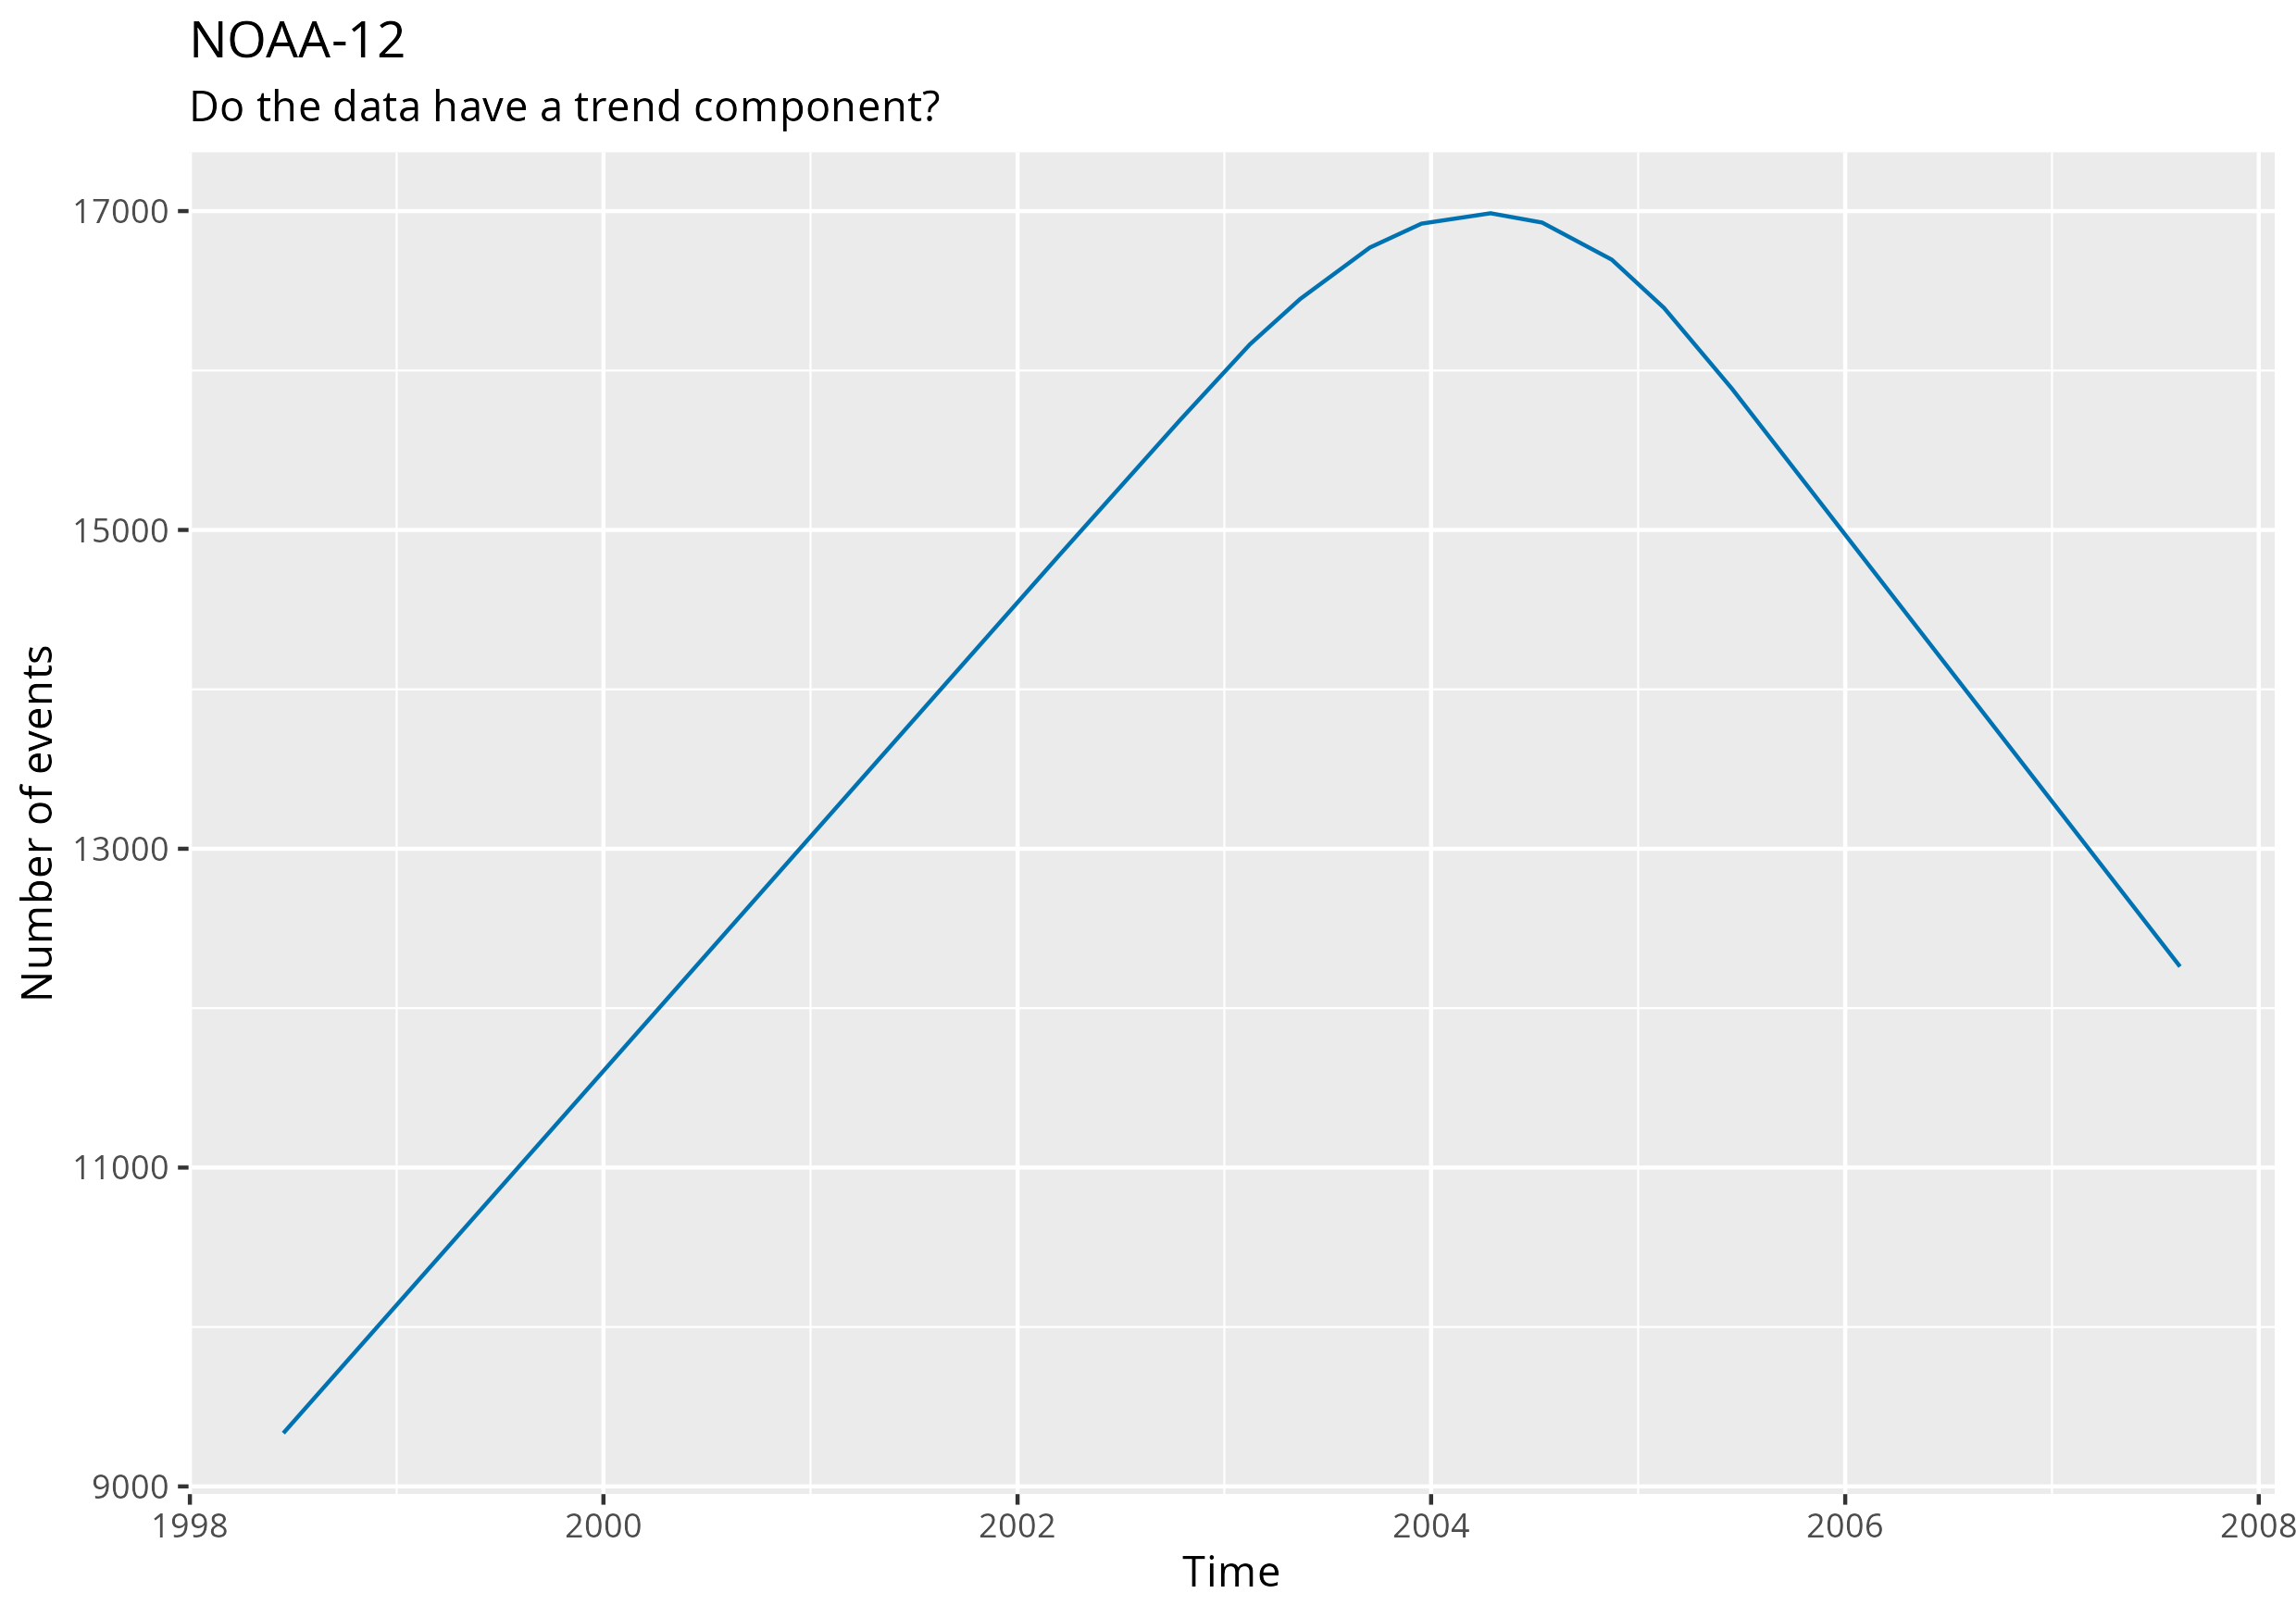
\includegraphics[scale=0.45]{figures/plot_component_trend_NOAA-12.png}
    \caption{Do the data have a trend component?}
  \end{figure}
\end{frame}

\begin{frame}
  \frametitle{Time series seasonality}
  \begin{figure}
    \centering
    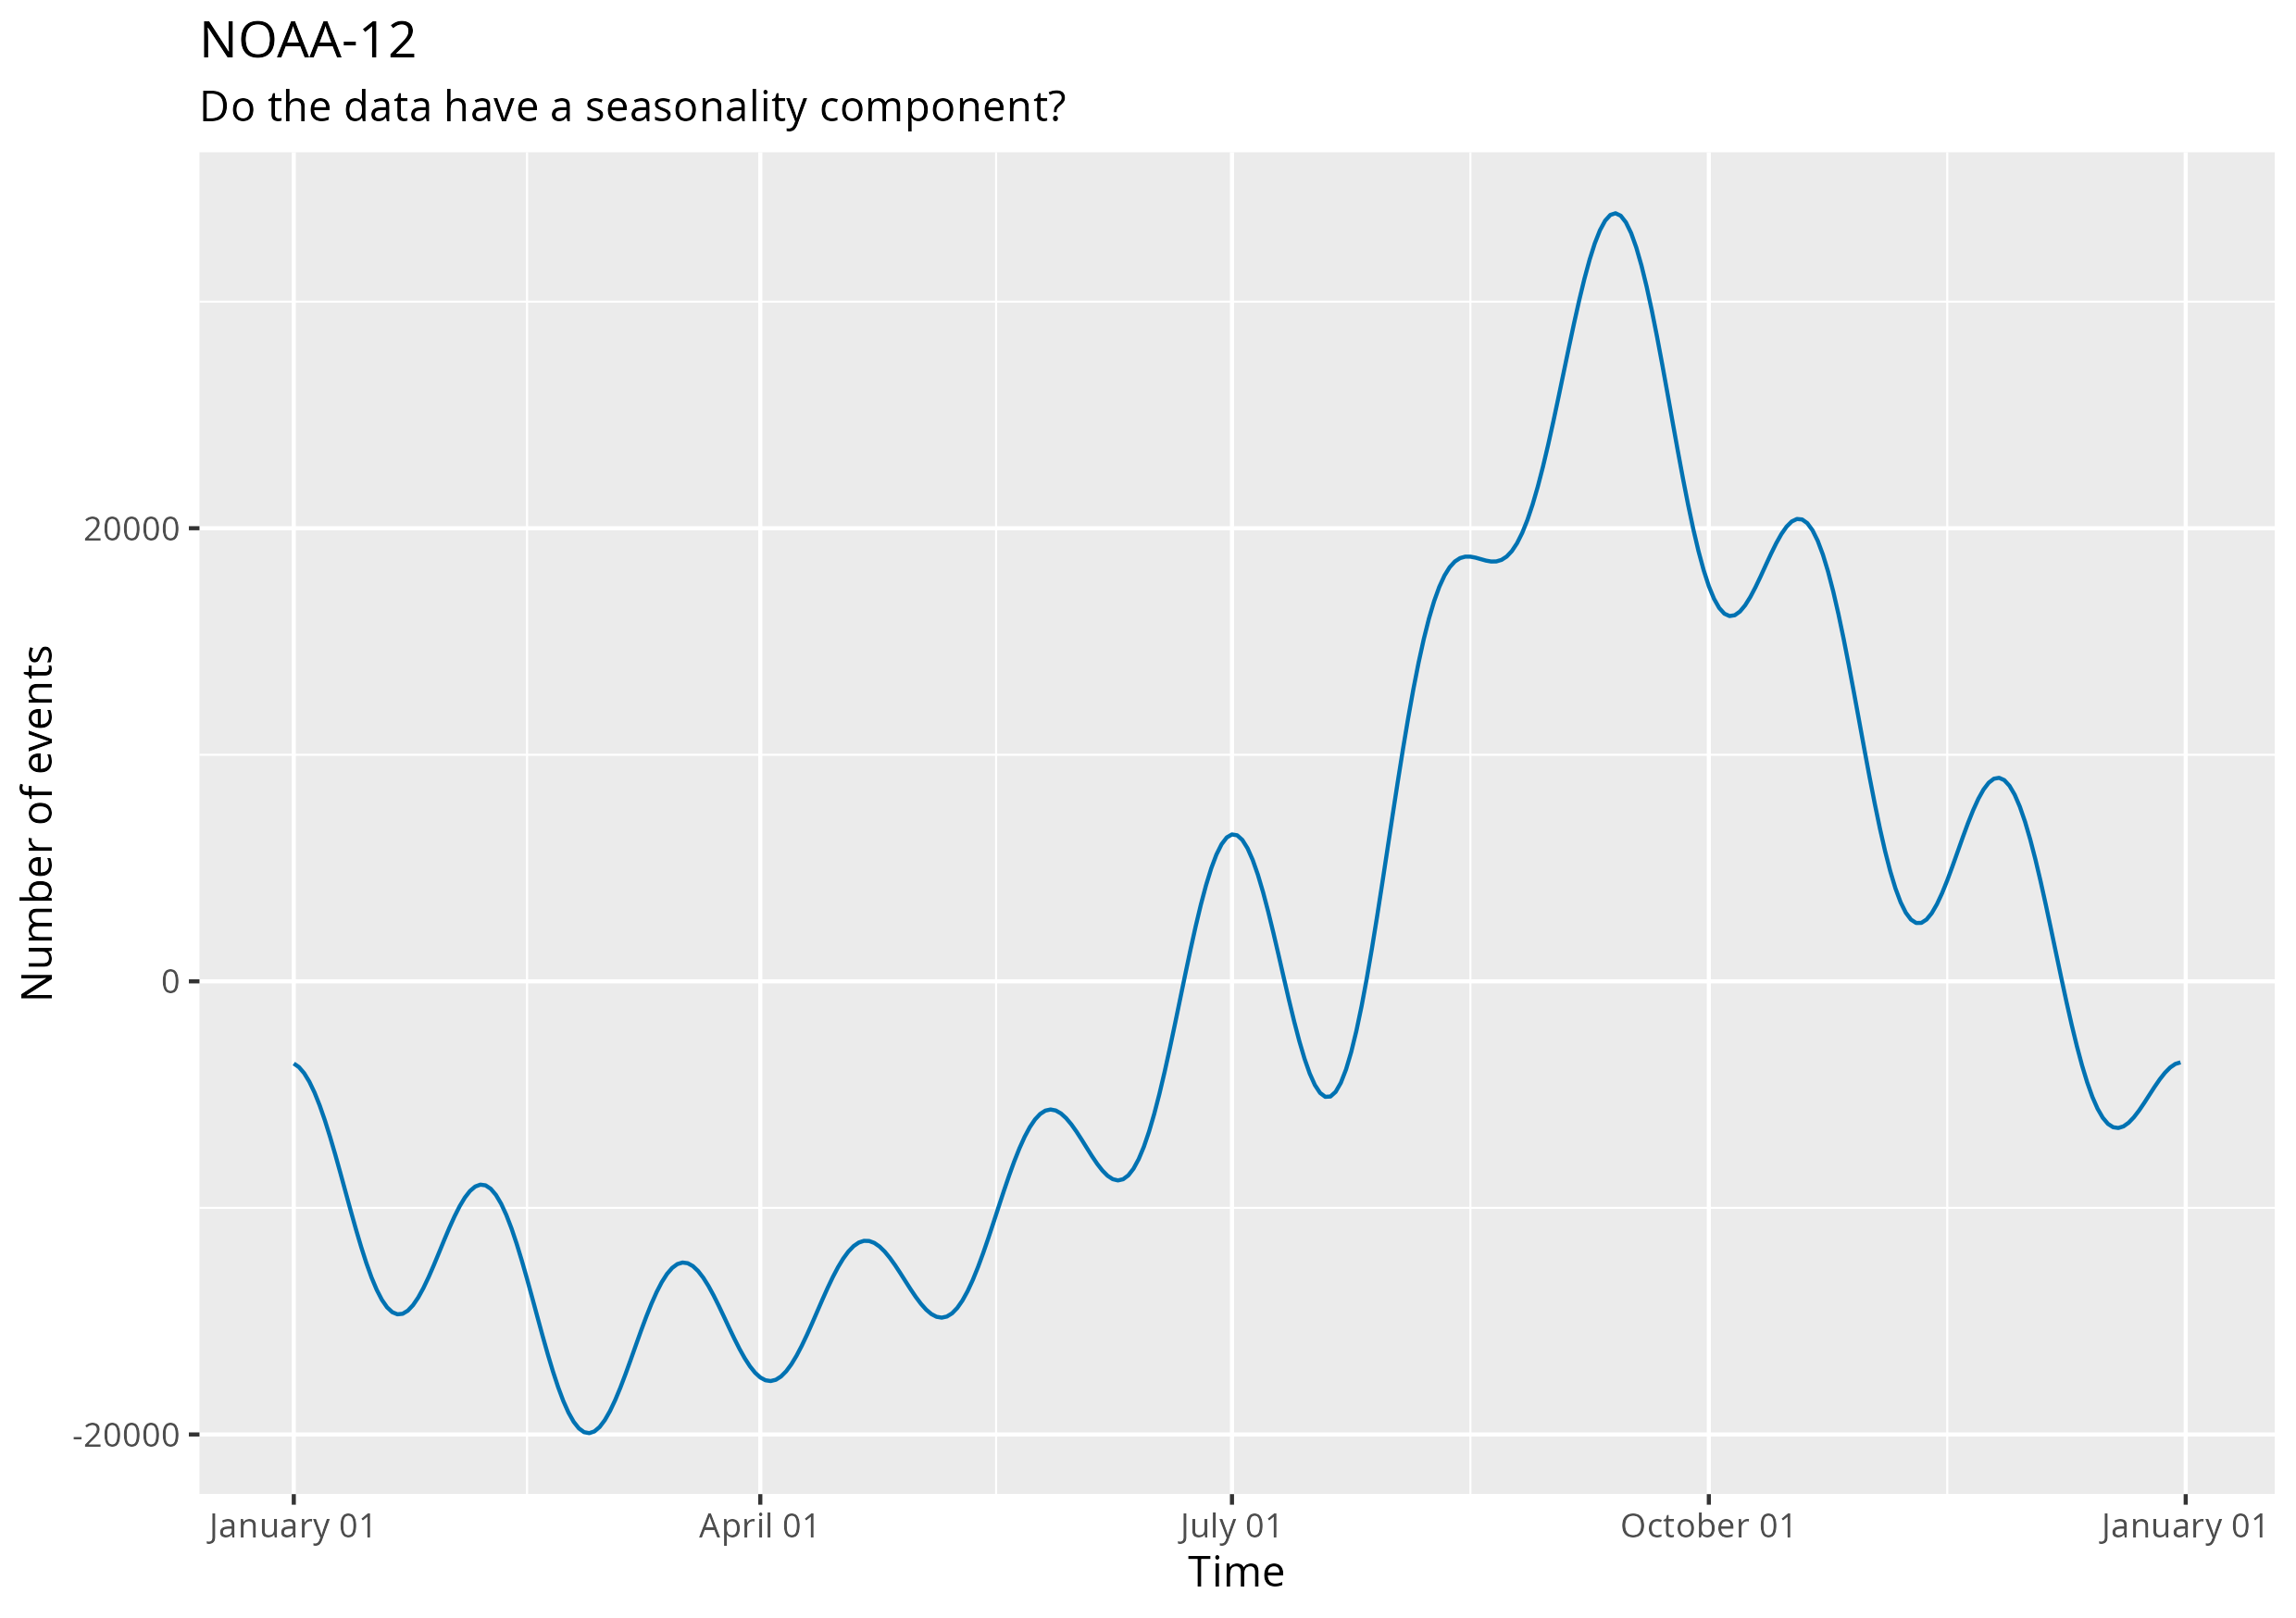
\includegraphics[scale=0.45]{figures/plot_component_seasonality_NOAA-12.png}
    \caption{Do the data have a seasonality component?}
  \end{figure}
\end{frame}

\begin{frame}
  \frametitle{Time series versus forecast}
  \begin{figure}
    \centering
    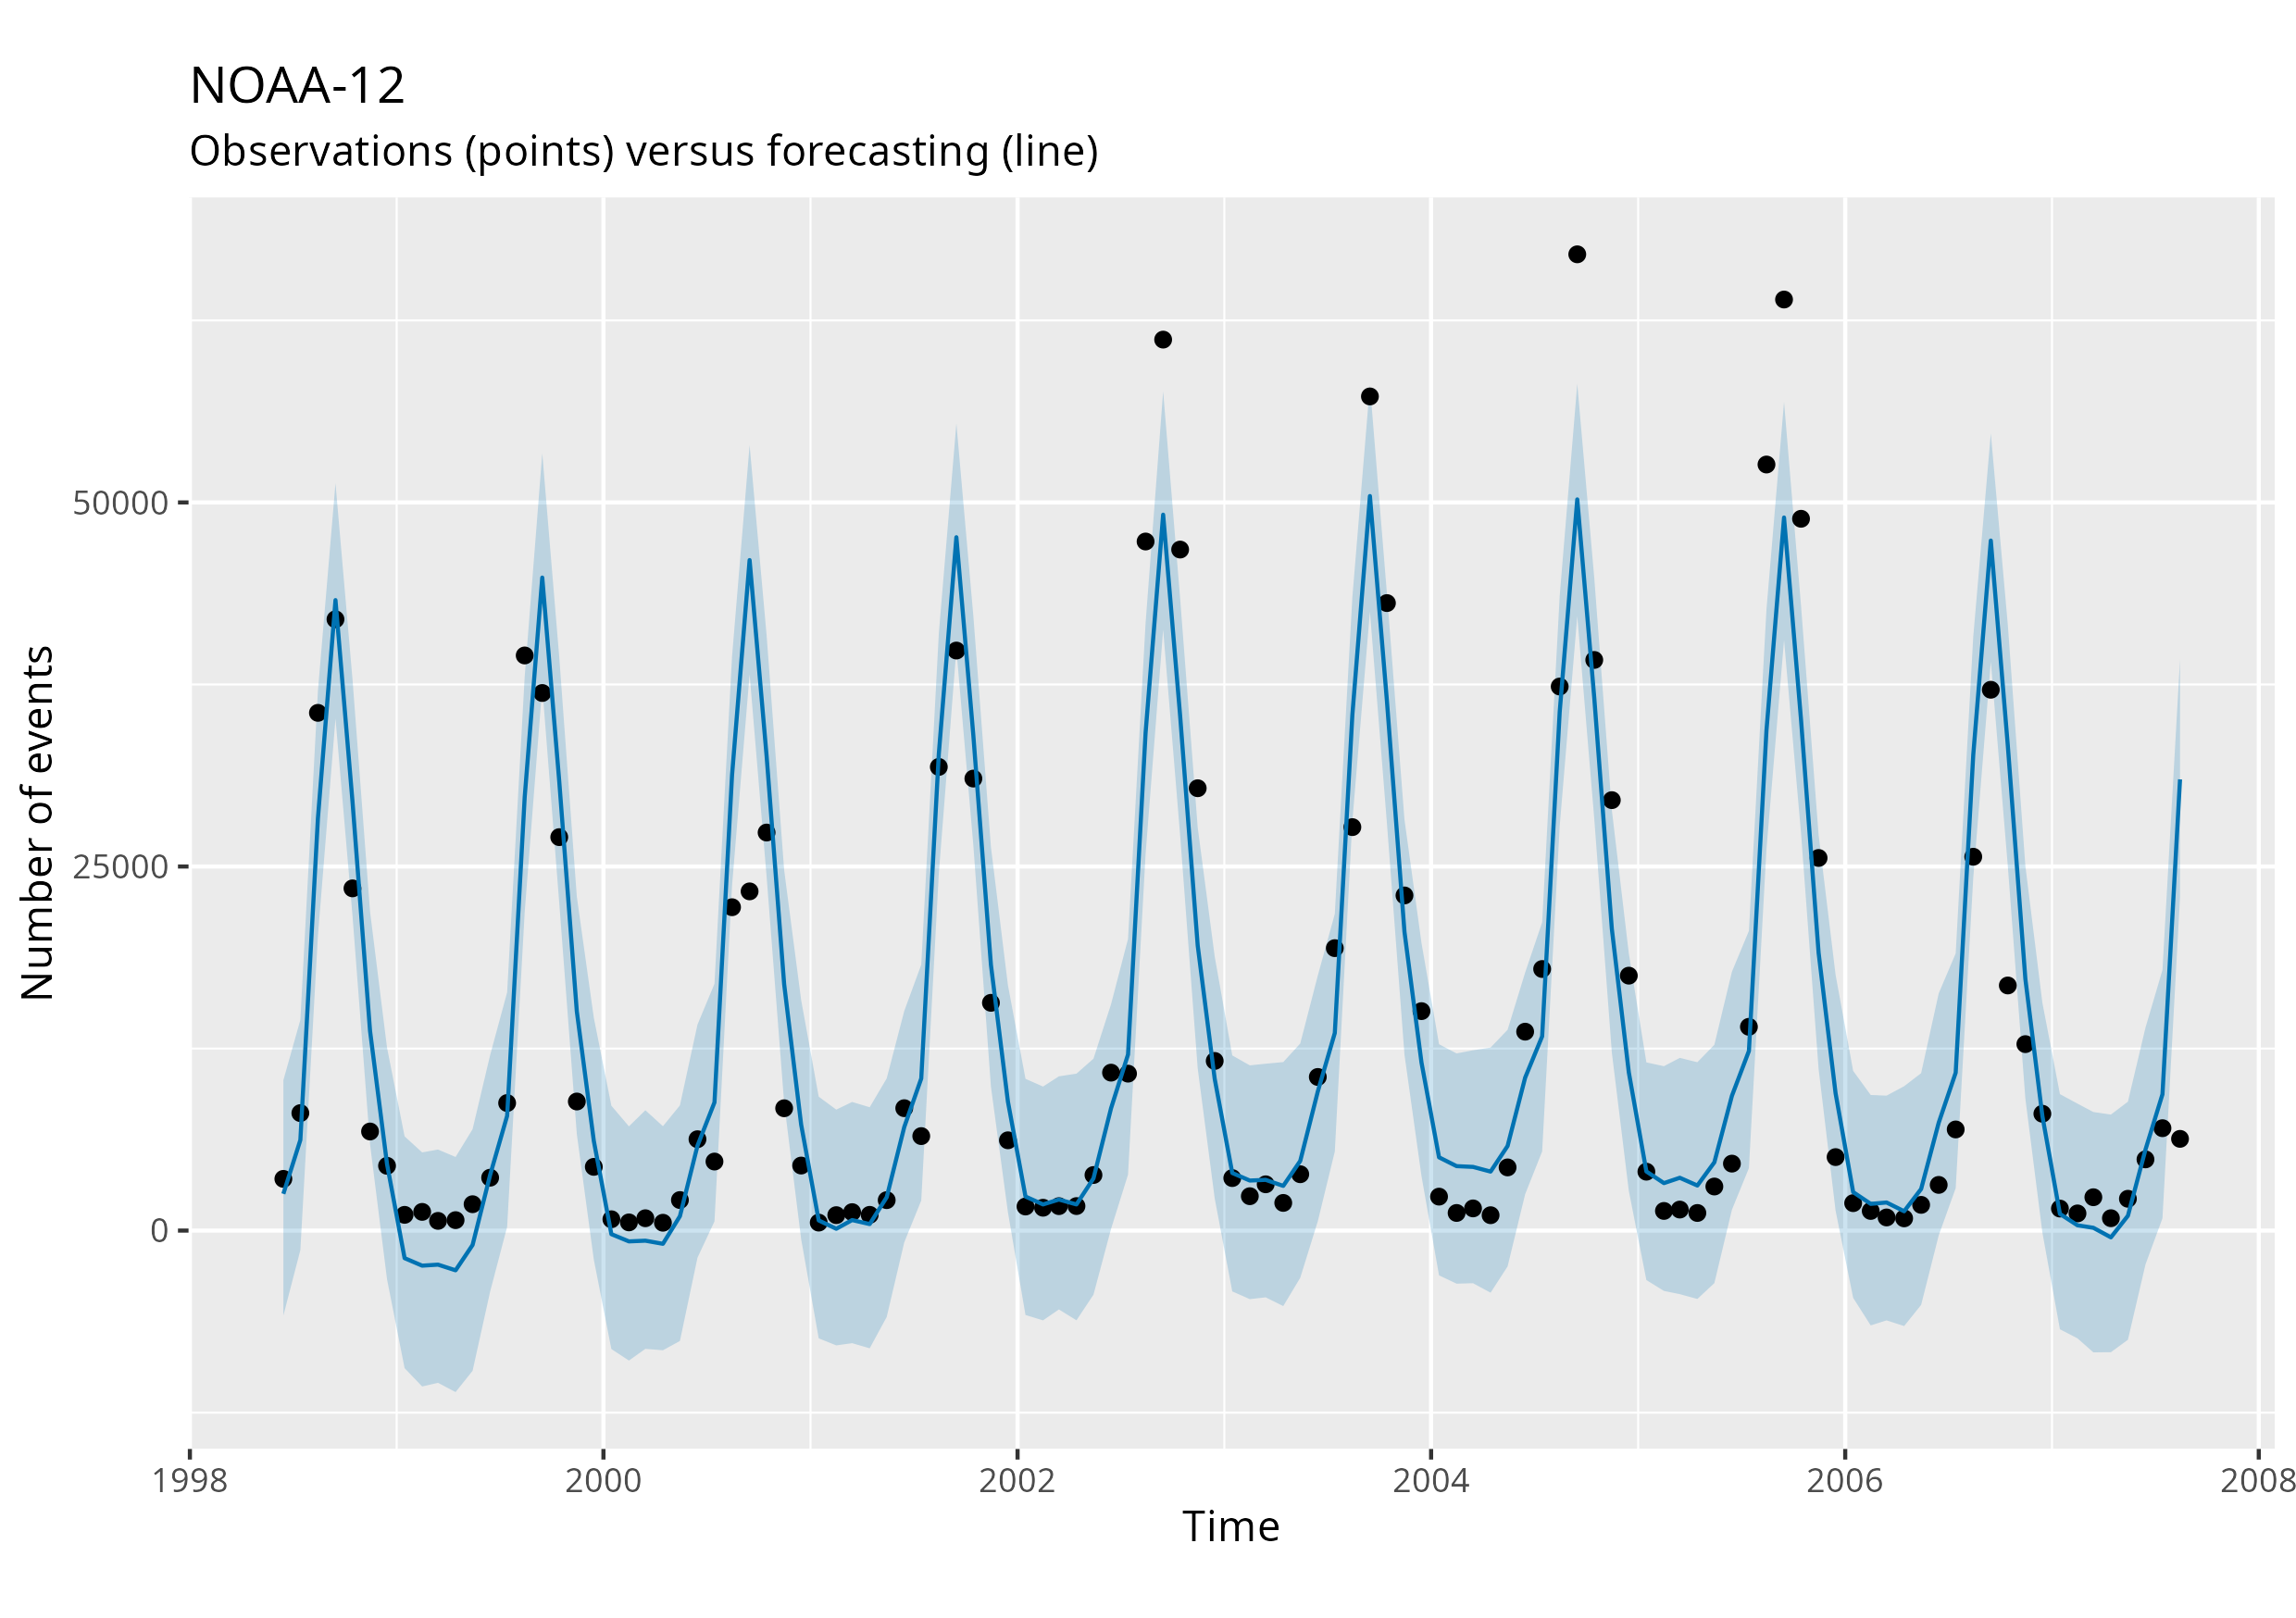
\includegraphics[scale=0.45]{figures/plot_model_forecast_NOAA-12.png}
    \caption{Observations (balck dots), model (blue line), and 95\% confidence
    interval (gray shadow).}
  \end{figure}
\end{frame}

\begin{frame}
  \frametitle{Time series versus forecast}
  \begin{figure}
    \centering
    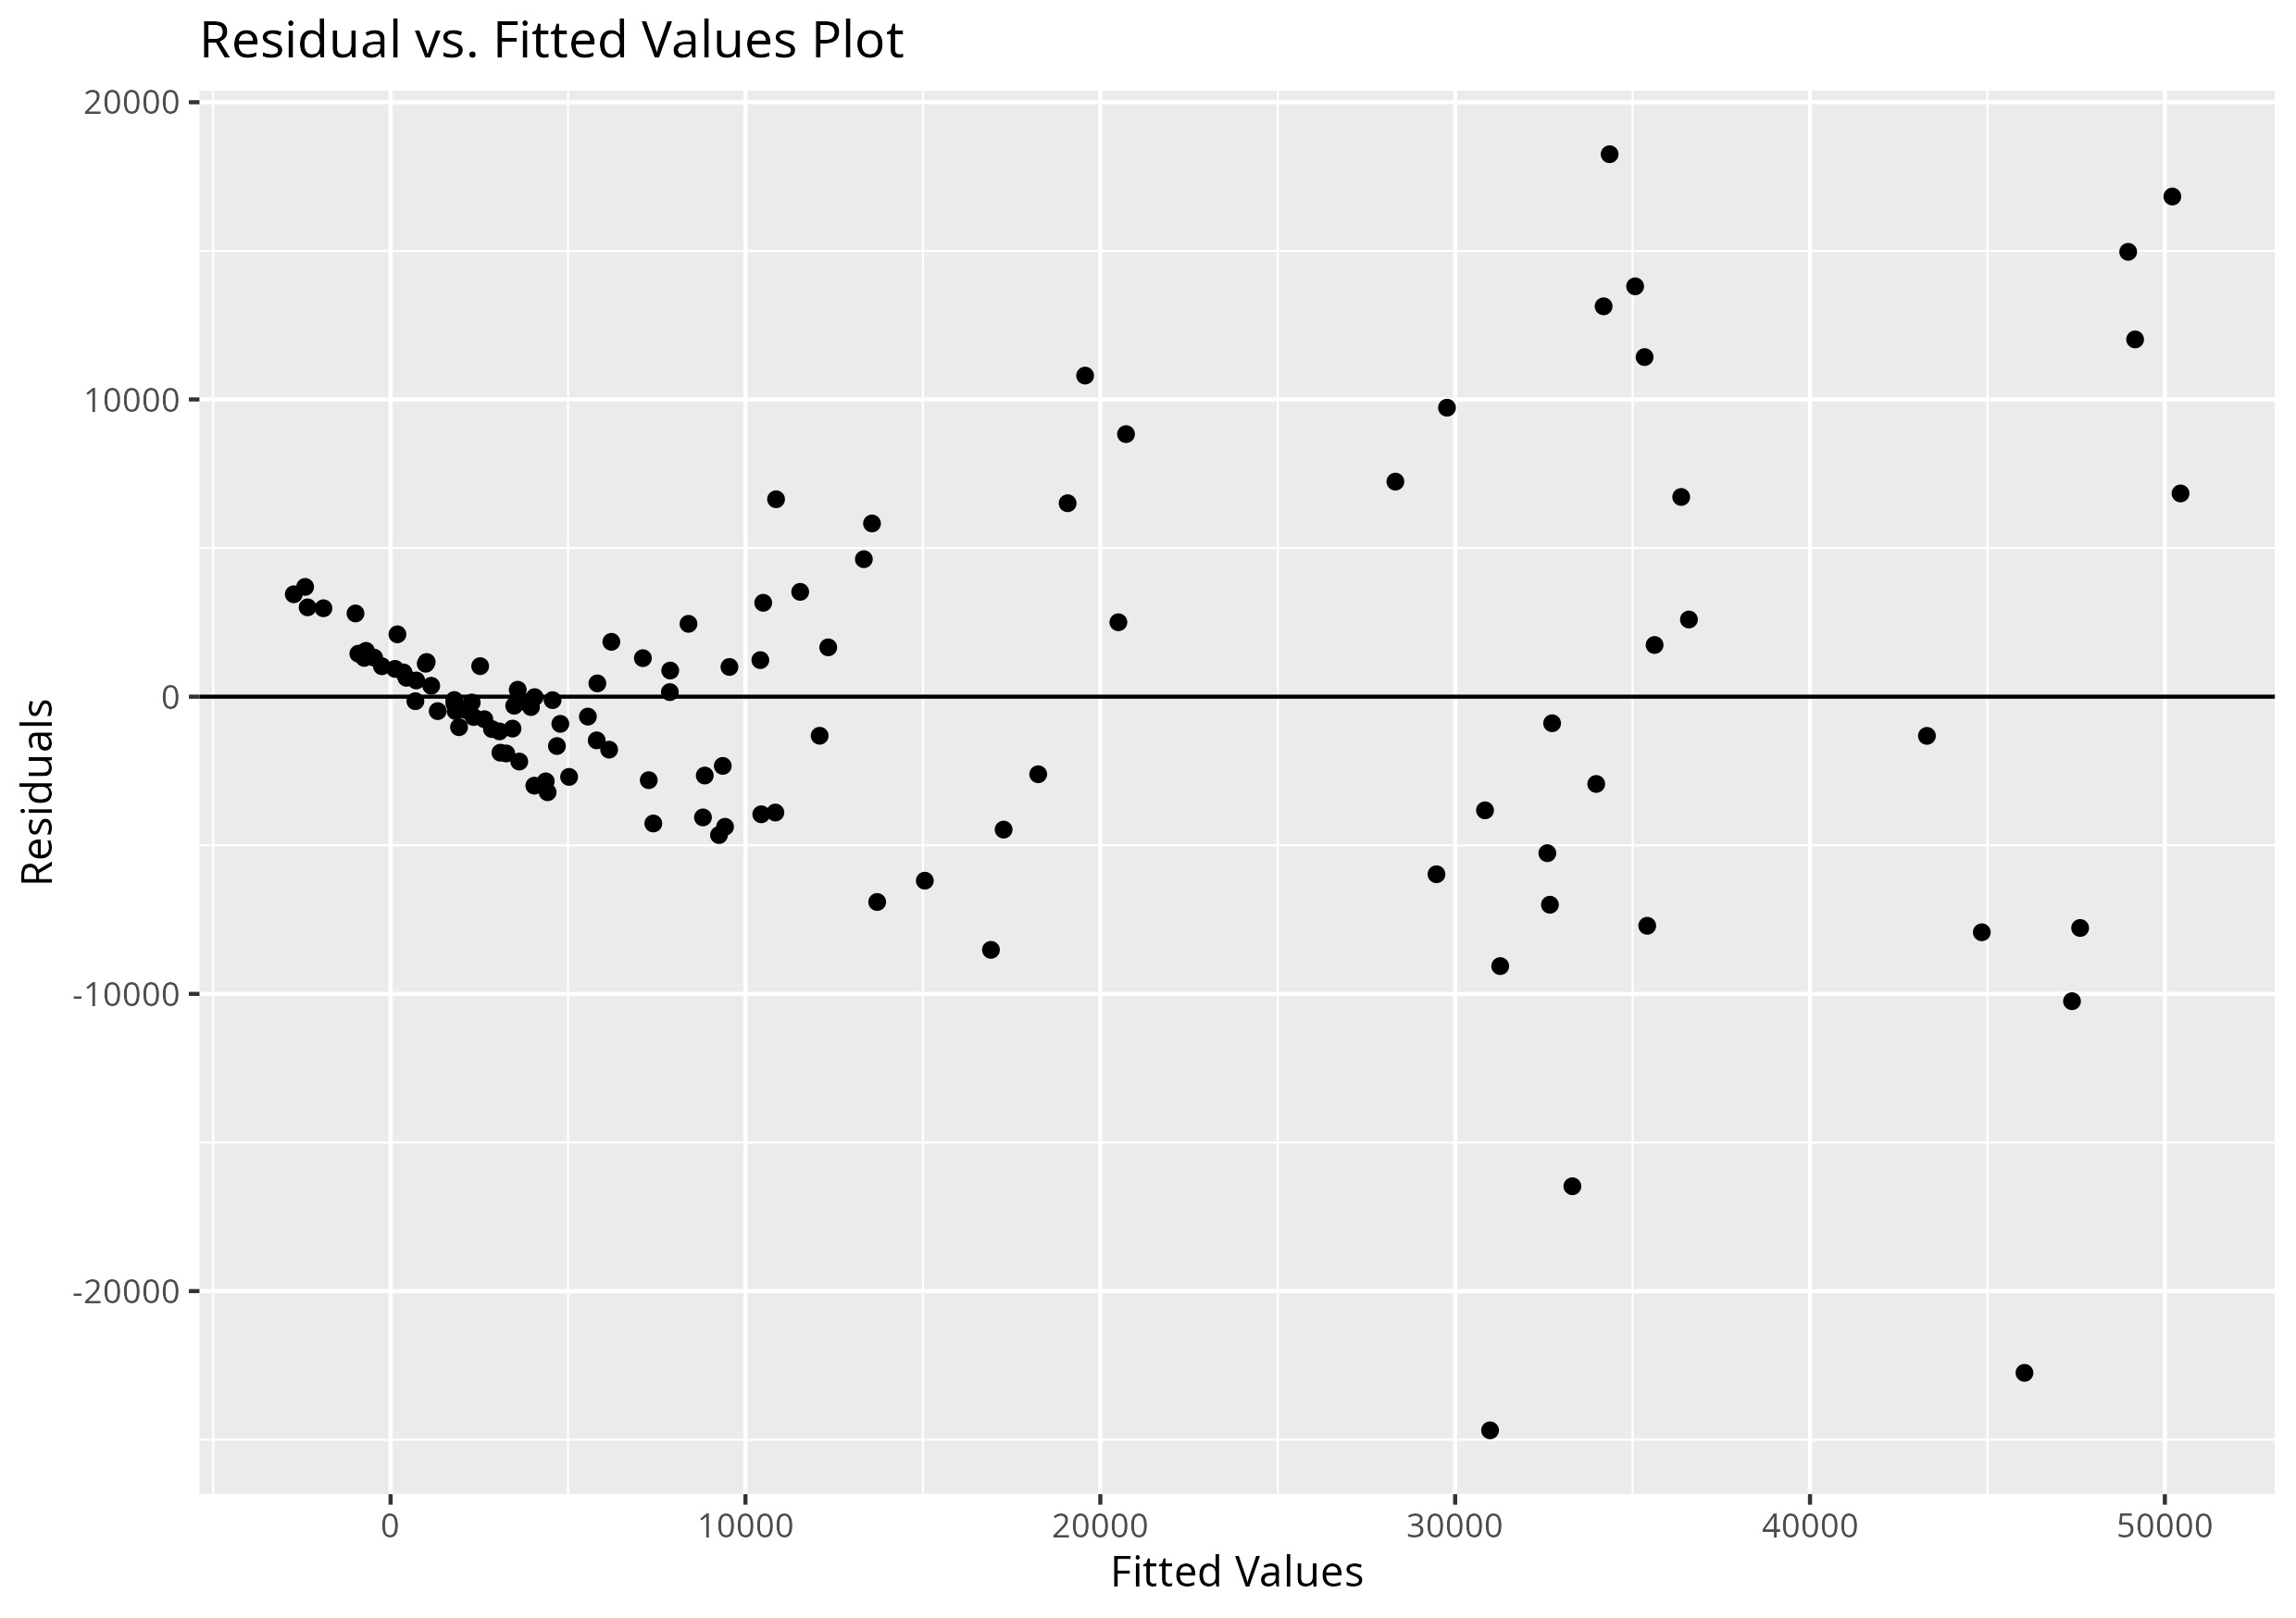
\includegraphics[scale=0.45]{figures/plot_residuals_NOAA-12.png}
    \caption{Large fitted fire foci values have large residuals.}
  \end{figure}
\end{frame}

\begin{frame}
  \frametitle{Time series versus forecast}
  \begin{figure}
    \centering
    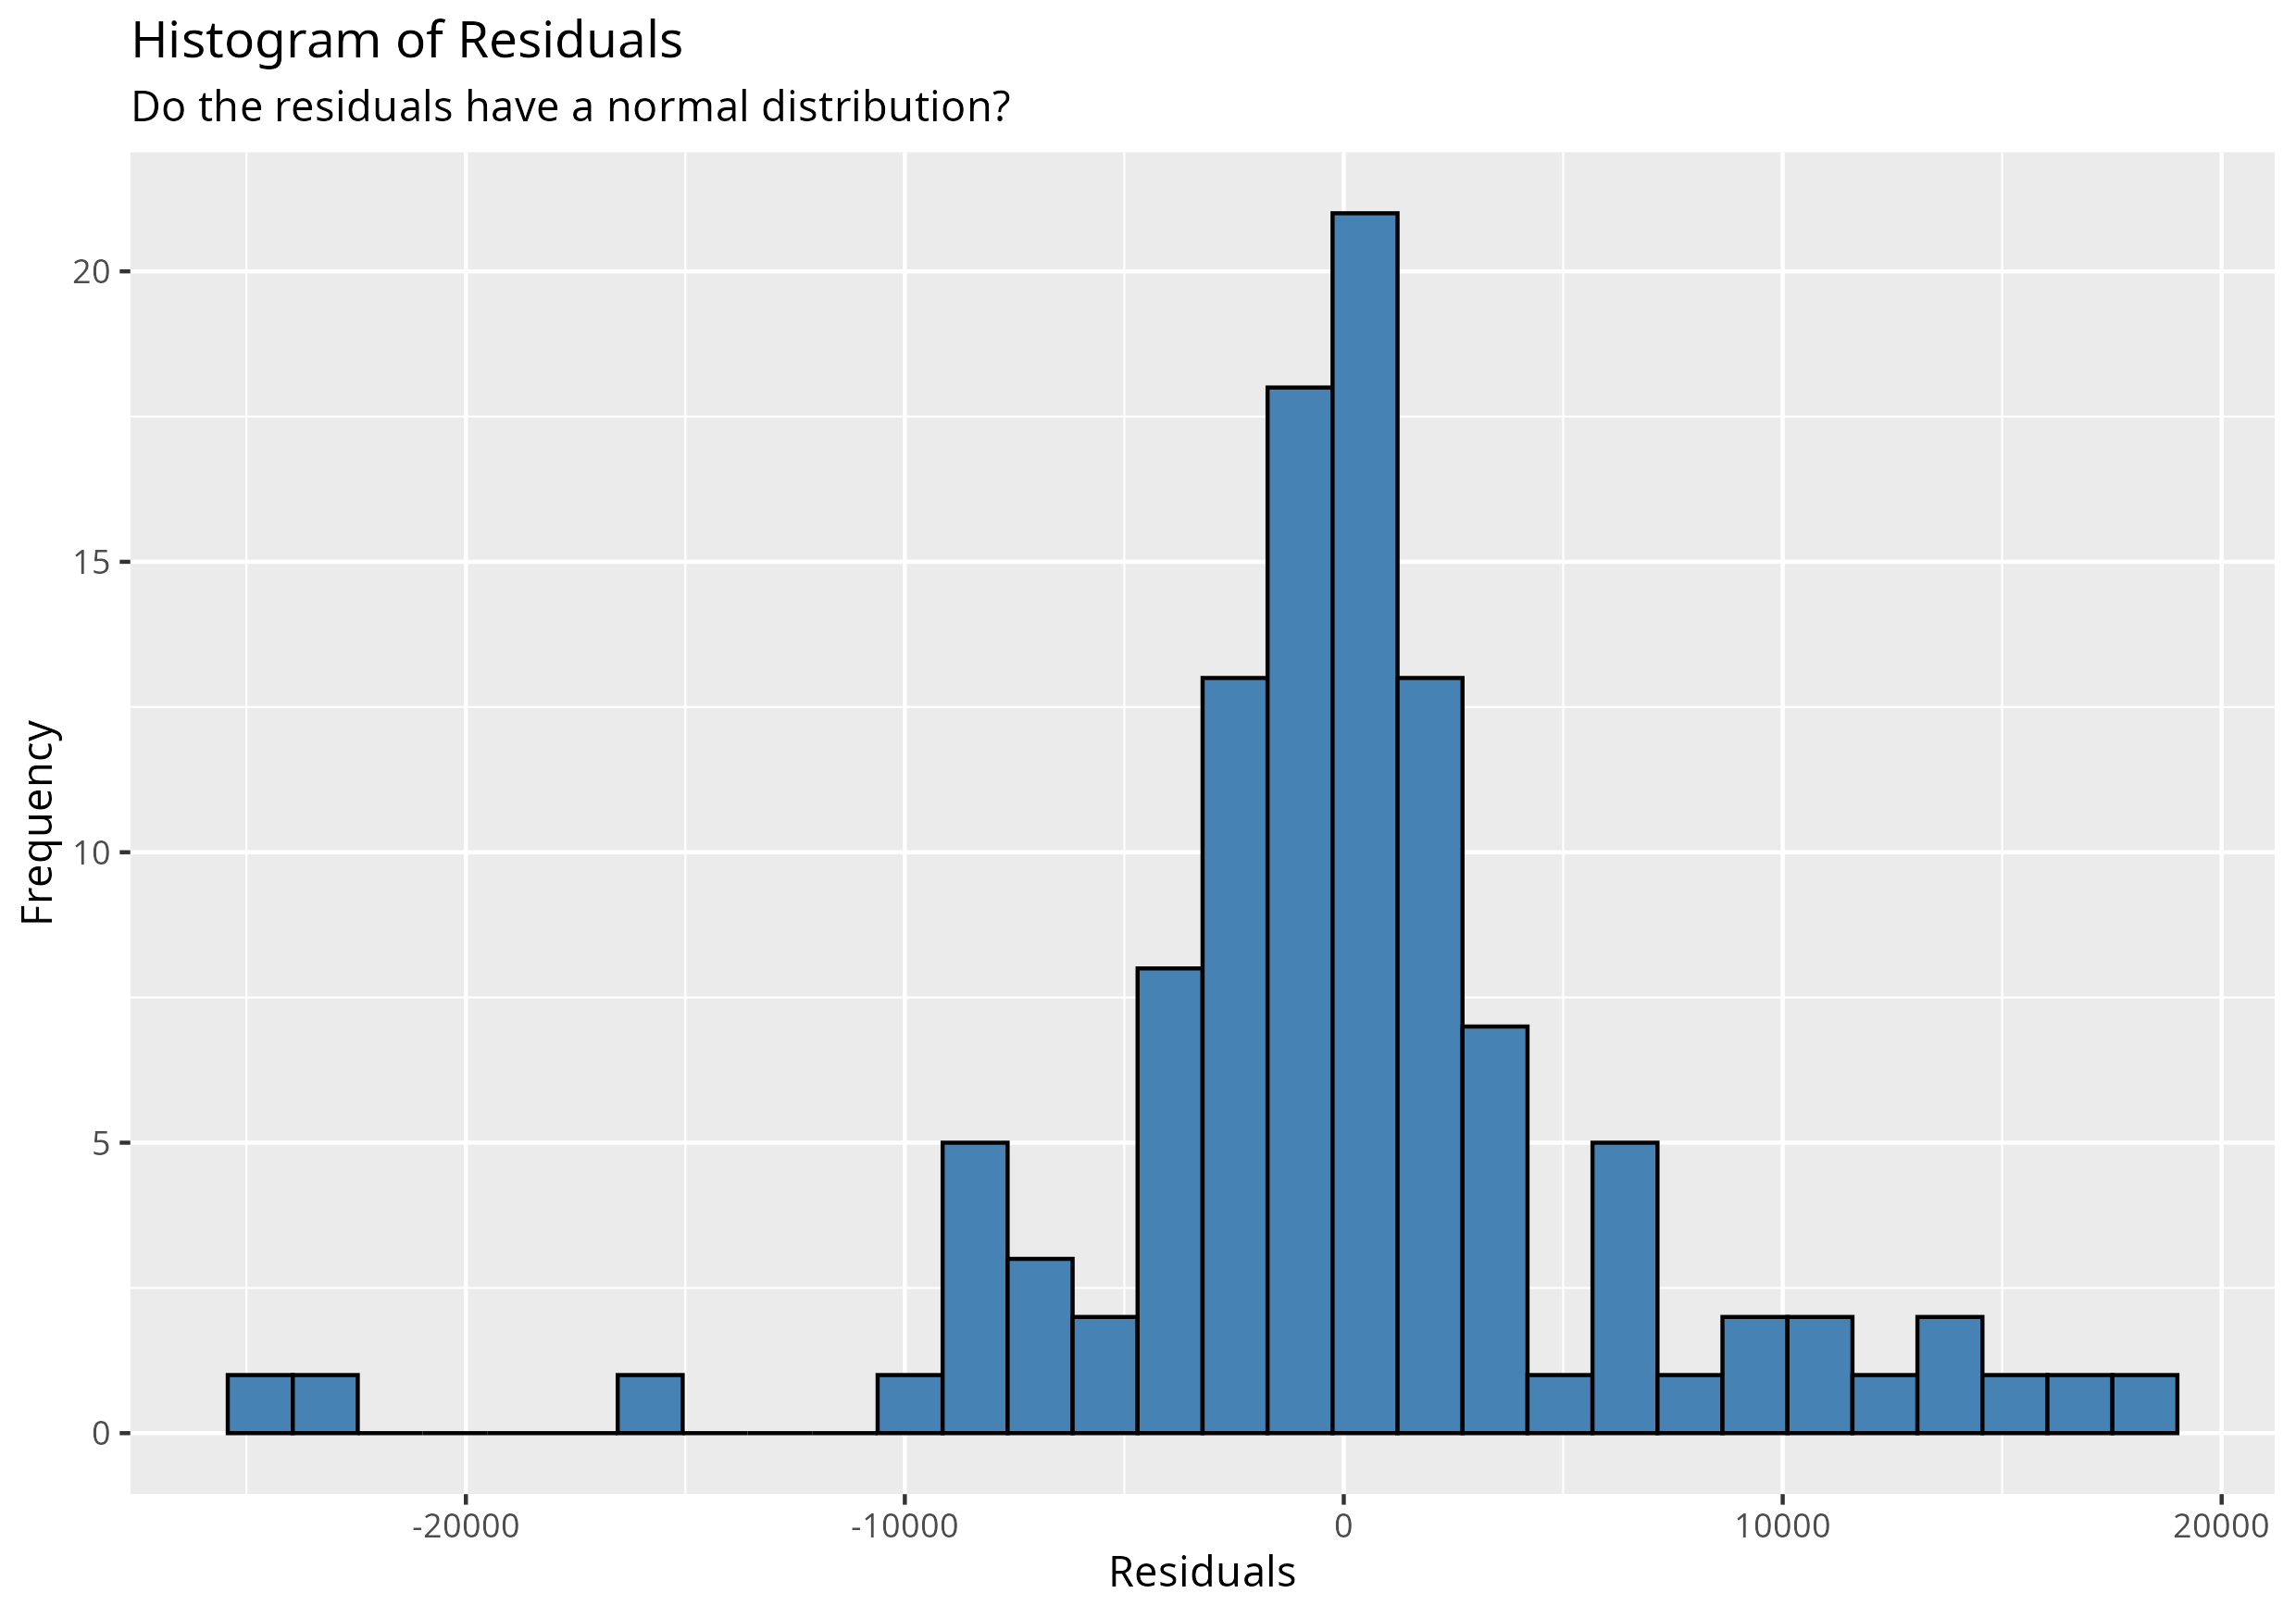
\includegraphics[scale=0.45]{figures/plot_residuals_hist_NOAA-12.png}
    \caption{Do the residuals have a normal distribution?}
  \end{figure}
\end{frame}

\begin{frame}
    \frametitle{Summary}
    \begin{table}
      \centering
      \csvautotabular{tables/check_models_summary.csv}
      \caption{Summary of findings in in the fire foci time series.}
    \end{table}
\end{frame}
